% !TeX document-id = {1f1cd383-6721-4950-8823-96b3144f4af7}
%!TEX program = xelatex 
% !BIB program = biber
%%%%%%%%%%%%%%%%%%%%%%%%%%%%%%%%%%%%%%%%%%%%%%%%%%
% 载入模版
%
% 载入 hutbthesis.cls文件定义的模板
%%%%%%%%%%%%%%%%%%%%%%%%%%%%%%%%%%%%%%%%%%%%%%%%%%

\documentclass[AutoFakeBold]{hutbthesis}

\addbibresource{content/reference.bib}

%%%%%%%%%%%%%%%%%%%%%%%%%%%%%%%%%%%%%%%%%%%%%%%%%%
% 基本信息
%
% 用户自行输入标题、作者等基本信息
% 都存储在\content\info.tex文件中
%%%%%%%%%%%%%%%%%%%%%%%%%%%%%%%%%%%%%%%%%%%%%%%%%%
%!TEX root = ../hutbthesis_main.tex
% 文章信息
\titlecn{湖南工商大学学位论文 } 
\titleen{Hunan University of Technology and Business Thesis \LaTeX{} Template v0.1}


%\minormajor{大数据与人工智能}
%\interestmajor{大数据与人工智能}
\author{张瀚驰}
\subsupervisor{}
\studentid{2123030023}
\priormajor{大数据与人工智能}
\myclass{数智2101班}
\supervisor{王海东\ 讲师}
\department{人工智能与先进计算学院}
\thesisdate{year=202, month=}

%以下的对本科生没有用
\clcnumber{TP391} 				% 中图分类号 Chinese Library Classification
\schoolcode{10533}			% 学校代码
\udc{004.9}						% UDC
\academiccategory{学术学位}	% 学术类

\begin{document}
%%%%%%%%%%%%%%%%%%%%%%%%%%%%%%%%%%%%%%%%%%%%%%%%%%
% 封面绘制
%
% 1.5版本重新编写了封面绘制宏,并用latex使用者更习惯的
% \maketitle代替之前的\makecoverpage
%%%%%%%%%%%%%%%%%%%%%%%%%%%%%%%%%%%%%%%%%%%%%%%%%%
\maketitle

%\declarationzh

% 启用大罗马字母进行编号
\frontmatter
% 设置页眉和页脚

%%!TEX root = ../csuthesis_main.tex
% 文章信息
\titlecn{湖南工商大学大学学位论文 \LaTeX{} }
\titleen{Hunan University Of Technology and Business Thesis \LaTeX{} }

\priormajor{}
\minormajor{}
\interestmajor{}
\author{张瀚驰}
\supervisor{王海东\ 讲师}
\subsupervisor{}
\department{人工智能与先进计算学院}
\studentid{2123030023}
\thesisdate{year=2025,month=5}
\myclass{大数据与人工智能}


%!TEX root = ../hutbthesis_main.tex

\begin{declarationzh}
		
本人郑重声明:所呈交的本科毕业设计 \uline{ 湖南工商大学学位论文 \LaTeX{} 模板使用示例 v0.1 } 是本人在指导老师的指导下,独立进行研究工作所取得的成果,成果不存在知识产权争议,除文中已经注明引用的内容外,本设计不含任何其他个人或集体已经发表或撰写过的作品成果。
对本设计做出重要贡献的个人和集体均已在文中以明确方式标明。本人完全意识到本声明的法律结果由本人承担。
	
	\vspace{30pt}
	\begin{tabular}{ll}
		%\renewcommand{\arraystretch}{2}
		\hspace{240pt} \makebox[4em][s]{作者签名:  颜磊  } & \underline{\makebox[100pt][c]{  }} \\
		\hspace{240pt} \makebox[4em][s]{日\qquad 期:}	 &
		\underline{\makebox[100pt][c]{\qquad2025年\quad1月\quad3日 }} \\
	\end{tabular}

	
	
\end{declarationzh}

% 授权书
%!TEX root = ../hutbthesis_main.tex

\keywordsen{HUTB\ \ LaTeX\ \ Template}
\begin{authorizationzh}
	
本毕业设计《基于数字孪生的自动驾驶强化学习仿真系统》是本人在校期间所完成学业的组成部分,是在学校教师的指导下完成的。
因此,本人特授权学校可将本毕业设计的全部或部分内容编入有关书籍、数据库保存,可采用复制、印刷、网页制作等方式将设计文本和经过编辑、批注等处理的设计文本提供给读者查阅、参考,可向有关学术部门和国家有关教育主管部门呈送复印件和电子文档。
本毕业设计无论做何种处理,必须尊重本人的著作权,署明本人姓名。
\\
\\
\\
\\
\\
\\
\\
\\

	
	\vspace{30pt}
	\begin{tabular}{llll}
		%\renewcommand{\arraystretch}{2}
		% \hspace{240pt} \makebox[4em][s]{设计作者(签字)} & \underline{\makebox[80pt][c]{  }} \\
		\makebox[4em][s]{设计作者(签字)} & \makebox[150pt][c]{  } & \makebox[2em][s]{时间} & \makebox[100pt][c]{\qquad 年\quad 月\quad   日 }\\
		\\ \\ \\
		\makebox[4em][s]{指导教师已阅(签字)} & \makebox[150pt][c]{  } & \makebox[2em][s]{时间} & \makebox[100pt][c]{\qquad 年\quad 月\quad   日 }\\
	\end{tabular}

	
	
\end{authorizationzh}

%%%%%%%%%%%%%%%%%%%%%%%%%%%%%%%%%%%%%%%%%%%%%%%%%%
% 中文摘要
%
% 存储在\content\abstractzh.tex文件中
%%%%%%%%%%%%%%%%%%%%%%%%%%%%%%%%%%%%%%%%%%%%%%%%%%
%!TEX root = ../csuthesis_main.tex
% 设置中文摘要
\keywordscn{智能驾驶\quad 仿真场景\quad 危险场景生成\quad NSGA-II 多目标优化}
%\categorycn{TP391}
\begin{abstractzh}

在智能驾驶系统的发展过程中,仿真场景的生成与优化是保障其安全性和可靠性的关键技术手段。本文首先基于自然驾驶数据提取具有代表性的危险场景,构建真实有效的仿真数据基础;随后,采用多维场景融合方法识别典型行车行为(如变道、跟车、邻车切入等),并与动态交通要素结合,生成更加复杂和真实的测试场景。针对现有测试环境中高风险场景覆盖率不足的问题,本文重点引入 NSGA-II 多目标优化算法,通过非支配排序与拥挤度计算,在“最小安全距离”和“碰撞风险”两个目标之间实现 Pareto 最优平衡,有效筛选出多样且具有代表性的高危场景。实验结果表明,与传统随机搜索方法相比,NSGA-II 可将高风险场景覆盖率提高 30\% 以上。最后,设计并实现了一套自动化仿真测试平台,集成场景生成、仿真执行、数据采集与结果分析功能,实现测试流程的自动化和标准化。本文方法显著提升了智能驾驶系统在仿真环境中的安全性验证能力,为未来自动驾驶系统的开发与测试提供了有力技术支撑。


\end{abstractzh}

%%%%%%%%%%%%%%%%%%%%%%%%%%%%%%%%%%%%%%%%%%%%%%%%%%
% 英文摘要
%
% 存储在\content\abstracten.tex文件中
%%%%%%%%%%%%%%%%%%%%%%%%%%%%%%%%%%%%%%%%%%%%%%%%%%
%!TEX root = ../csuthesis_main.tex
\keywordsen{Brain-inspired vision;\ \ CORnet model;\ \ Channel attention;\ \ Brain-Score evaluation;\ \ Neural response similarity}
\begin{abstracten}

Brain-inspired visual models aim to simulate the information processing mechanisms of the human visual cortex and play a significant role in the interdisciplinary research between computer vision and neuroscience. This study is based on the CORnet model family and focuses on two main aspects: recognition performance optimization and brain-likeness analysis. First, the CORnet-S model was reproduced on the Tiny-ImageNet dataset to verify its image recognition ability under a lightweight architecture. Then, a modified model named CORnet-Z+SE was constructed by introducing a Squeeze-and-Excitation (SE) channel attention mechanism into the CORnet-Z model. Experimental results show that both Top-1 and Top-5 accuracy improved to a certain extent.

To evaluate the brain-likeness of the models, this study employed the Brain-Score framework and used the publicly available MajajHong2015 neural dataset to assess representational similarity in the V4 and IT brain regions. Results indicate that although the introduction of attention mechanisms improved classification accuracy, it led to a decline in brain similarity scores, suggesting a trade-off between discriminative performance and neural alignment. Visualization of activation maps further showed that the SE module enhanced the model’s response to local target regions, but may have reduced the breadth of overall activation, potentially affecting its biological plausibility.

\end{abstracten}



%%%%%%%%%%%%%%%%%%%%%%%%%%%%%%%%%%%%%%%%%%%%%%%%%%
% 目录
%
% 使用重定义的tableofcontents宏绘制目录
% 满足学校的样式要求
%%%%%%%%%%%%%%%%%%%%%%%%%%%%%%%%%%%%%%%%%%%%%%%%%%
\tableofcontents


% 启用数字编号,改为第 x 页  共 x 页格式
\mainmatter

%%%%%%%%%%%%%%%%%%%%%%%%%%%%%%%%%%%%%%%%%%%%%%%%%%
% 正文
%
% 存储在\content\content.tex文件中
%%%%%%%%%%%%%%%%%%%%%%%%%%%%%%%%%%%%%%%%%%%%%%%%%%
% 正文
%%!TEX root = ../hutbthesis_main.tex

%子章节为了便于查找和修改,建议通过input拆分文件

%%%%%%%%%%%%%%%%%%%%%%%%%%%%%%%%绪论%%%%%%%%%%%%%%%%
 \documentclass{article}
\usepackage{amsmath}
\usepackage{amssymb}
\usepackage{enumitem} % 用于自定义列表样式
\usepackage{hyperref} % 用于添加超链接(可选)
\usepackage{lipsum} % 用于生成示例文本,实际使用中可移除
\usepackage{ctex} % 支持中文
\usepackage{amsmath} % 支持数学公式
\usepackage{enumitem} % 用于自定义列表样式
\usepackage{geometry} % 支持页面布局设置
\geometry{a4paper,scale=0.8} % 设置A4纸和缩放

\title{基于预训练大模型的高保真三维智能驾驶场景生成系统}
\author{郑睿翔}

\begin{document}

\section*{选题价值}

在探讨选题价值时,我们主要关注的是该选题是否具有创新性、实用性、可行性以及其对相关领域或社会的潜在影响。

\subsection*{创新性}
该选题结合了当前人工智能领域的多个前沿技术,如预训练大模型、自然语言处理(通过ChatSim)、高级仿真(CARLA)和目标检测(YOLO)。这些技术的融合在智能驾驶系统中是新颖的。利用自然语言命令生成和编辑高保真三维驾驶场景的方法,为智能驾驶系统的测试和开发提供了新的视角和工具,这在以前是没有被充分探索的。

\subsection*{实用性}
高保真三维智能驾驶系统能够为自动驾驶技术的研发提供一个接近真实世界的测试环境,有助于加速技术的成熟和商业化进程。通过在虚拟环境中进行大量的模拟测试,可以在不实际上路的情况下发现潜在的安全问题,从而降低自动驾驶车辆在实际应用中的风险。

\subsection*{可行性}
预训练大模型、CARLA仿真环境和YOLO目标检测算法都已经有了相对成熟的技术基础,这为该选题的实施提供了坚实的基础。这些技术和工具大多是开源的,或者可以通过商业途径获取,因此资源获取相对容易。

\subsection*{潜在影响}
该选题的成功实施有望推动自动驾驶技术向更高层次发展,提高自动驾驶系统的性能和安全性。随着自动驾驶技术的不断进步,将带动汽车制造、传感器技术、人工智能算法等相关产业的发展。自动驾驶技术的普及将改变人们的出行方式,提高交通效率,减少交通事故,对社会产生深远影响。


\section{文献综述}
随着人工智能技术的飞速发展,特别是预训练大模型在自然语言处理(NLP)和计算机视觉(CV)等领域的广泛应用,智能驾驶技术迎来了新的突破。高保真三维智能驾驶场景生成系统作为智能驾驶技术的重要组成部分,对于提升自动驾驶系统的安全性和可靠性具有重要意义。本文旨在综述国内外关于基于预训练大模型的高保真三维智能驾驶场景生成系统的研究状况和发展趋势,并探讨这些研究对本人工作的启发。

\section{国内外研究状况}

\subsection{国内研究状况}
近年来,国内在智能驾驶技术方面取得了显著进展,特别是在预训练大模型和高保真三维场景生成方面。国内企业和研究机构纷纷投入大量资源,推动相关技术的发展和应用。

\begin{enumerate}[label=\arabic*.]
    \item 华为推出的盘古系列超大预训练模型,包括中文语言(NLP)、视觉(CV)大模型、多模态大模型和科学计算大模型,旨在建立一套通用、易用的人工智能开发工作流,赋能更多的行业和开发者,实现人工智能工业化开发。盘古大模型在智能驾驶场景生成中的应用,可以显著提升场景的逼真度和复杂性,为自动驾驶系统的训练和测试提供有力支持。
    \item 北京智源人工智能研究院发布的超大规模智能模型“悟道2.0”,达到1.75万亿参数,成为全球最大的预训练模型之一。该模型在智能驾驶场景生成中的应用潜力巨大,可以通过对大规模数据的训练,生成高度逼真的三维场景,为自动驾驶系统的优化和验证提供重要支持。
    \item 清华大学智能产业研究院(AIR)在构建Real2Sim2Real基础模型平台、自动驾驶仿真平台等方面取得了显著成果。其中,Real2Sim2Real平台通过结合真实世界数据和仿真数据,利用预训练大模型生成高保真三维智能驾驶场景,为自动驾驶系统的训练和测试提供了有力保障。
    \item YOLO(You Only Look Once)模型在国内得到了广泛的关注和应用。随着YOLO模型的迭代升级,其在国内的应用场景也不断拓展,涵盖了安防监控、无人驾驶、医疗诊断等多个领域。
    \item CARLA仿真平台在国内得到了广泛的应用和认可。作为国内自动驾驶领域的重要工具之一,CARLA为自动驾驶系统的开发、训练和验证提供了有力的支持。
    \item ChatSim项目在国内尚处于起步阶段,但已经引起了广泛的关注和兴趣。作为国内首个通过大语言模型实现可编辑逼真3D驾驶场景仿真的项目,ChatSim为自动驾驶场景仿真提供了新的思路和方法。
\end{enumerate}

\subsection{国外研究状况}
国外在基于预训练大模型的高保真三维智能驾驶场景生成系统方面也取得了显著进展。

\begin{enumerate}[label=\arabic*.]
    \item OpenAI推出的GPT系列模型,特别是GPT-3,以其1750亿参数规模的预训练模型,展示了强大的零样本与小样本学习能力。这些能力在智能驾驶场景生成中具有重要应用潜力,可以通过对少量标注数据的训练,生成高度逼真的三维场景。
    \item 谷歌在预训练大模型方面也取得了重要进展。谷歌推出的Switch Transformer模型,以高达1.6万亿的参数量打破了GPT-3作为最大AI模型的统治地位,成为史上首个万亿级语言模型。该模型在智能驾驶场景生成中的应用,可以显著提升场景的复杂性和多样性,为自动驾驶系统的训练和测试提供更多可能性。
    \item 微软亚洲研究院提出的NÜwa模型,是一个可以同时覆盖语言、图像和视频的统一多模态预训练模型。该模型在文档理解、图像生成等方面取得了显著成果,为智能驾驶场景生成中的多模态数据融合提供了有力支持。
    \item YOLO模型在国外同样受到了广泛的关注和应用。自YOLOv1发布以来,其已经经历了多轮迭代,每一次更新都在精度和速度上取得了显著的进步。
    \item CARLA仿真平台在国外同样受到了广泛的关注和应用。作为自动驾驶领域的重要工具之一,CARLA为自动驾驶技术的研发提供了有力的支持。
    \item ChatSim项目在国外同样处于起步阶段,但已经取得了一定的研究成果和进展。国外的研究机构和企业在ChatSim的基础上进行了深入的研究和改进,提高了其性能和精度。
\end{enumerate}

\section{发展趋势}
基于预训练大模型的高保真三维智能驾驶场景生成系统的发展趋势主要体现在以下几个方面:

\begin{enumerate}[label=\arabic*.]
    \item 更大规模的预训练模型将成为未来发展的重要方向。更大规模的模型可以学习更多复杂的知识和特征,生成更加逼真的三维智能驾驶场景。
    \item 多模态数据融合将受到更多关注,以提高场景生成的逼真度和准确性。
    \item 强化学习与生成式AI的结合将成为研究热点,以提升自动驾驶系统的安全性和可靠性。
    \item 仿真与真实世界的互动将更加紧密,通过构建仿真平台将真实世界的数据和仿真数据相结合。
\end{enumerate}

\section{本人的思考}
基于预训练大模型的高保真三维智能驾驶系统是一个复杂且高度集成的系统,它涉及多个组件和技术的协同工作。ChatSim、CARLA和YOLO都是在这一领域中具有重要潜力的工具和技术。我将用以下这三个工具来构建高保真三维智能驾驶系统:

\begin{enumerate}[label=\arabic*.]
    \item \textbf{ChatSim}:
        \begin{itemize}
            \item 功能概述:ChatSim是一个革命性的开源项目,它首次实现了通过自然语言命令编辑出照片级真实的三维驾驶场景模拟,且能与外部数字资产无缝集成。这是通过大型语言模型(LLM)代理协作框架实现的,允许用户使用自然语言来控制和编辑复杂的驾驶场景,创造出高度逼真的视频。
            \item 在高保真三维智能驾驶系统中的应用:ChatSim可以作为系统的一部分,用于生成和编辑驾驶场景。通过自然语言命令,用户可以轻松地创建和修改各种驾驶环境,包括道路、车辆、行人和其他交通元素。这种灵活性对于测试和开发自动驾驶算法至关重要。
        \end{itemize}
    \item \textbf{CARLA仿真平台(0.9.15)}:
        \begin{itemize}
            \item 功能概述:CARLA是一个基于虚幻引擎的开源自动驾驶模拟器,支持实时模拟、多传感器数据和高度定制化环境。它提供了高度可定制的环境,让研究人员和开发者能够在各种复杂场景中测试和训练他们的算法。
            \item 在高保真三维智能驾驶系统中的应用:CARLA可以作为系统的主要模拟环境,提供高保真的3D环境、实时的仿真速度和多种虚拟传感器数据。这些功能使得CARLA成为测试和开发自动驾驶算法的理想平台。此外,CARLA的开源特性使得开发者可以深入理解其工作原理,并根据需要进行修改和扩展。
        \end{itemize}
    \item \textbf{YOLO模型}:
        \begin{itemize}
            \item 功能概述:YOLO(You Only Look Once)是一种流行的目标检测算法,以其高效和准确性而闻名。YOLO-BEV是YOLO的一个变体,专门设计用于生成车辆环境的鸟瞰图(BEV),这对于自动驾驶系统来说是一个重要的功能。
            \item 在高保真三维智能驾驶系统中的应用:YOLO(特别是YOLO-BEV)可以作为系统的一部分,用于车辆感知和目标检测。通过处理来自多个摄像头的图像数据,YOLO-BEV可以生成车辆环境的鸟瞰图,为自动驾驶系统提供更全面的环境信息。这有助于系统更准确地识别道路、车辆、行人和其他障碍物,从而提高自动驾驶的安全性和可靠性。
        \end{itemize}
\end{enumerate}

\section{结论}
基于预训练大模型的高保真三维智能驾驶场景生成系统是智能驾驶技术的重要组成部分。本文综述了国内外在该领域的研究状况和发展趋势,并探讨了这些研究对本人工作的启发。未来的研究将更加注重更大规模的预训练模型、多模态数据融合、强化学习与生成式AI的结合以及仿真与真实世界的互动等方面的发展。通过不断探索和创新,我们可以为自动驾驶系统的安全性和可靠性提供有力保障,推动智能驾驶技术的不断进步和发展。
\section{参考文献}
\begin{thebibliography}{99}
    \bibitem{li2018} 李欣儒. 以智能驾驶为例浅析计算机通信技术与电子信息在人工智能领域的实践应用[J]. 中国战略新兴产业,2018(8).
    \bibitem{yang2014} 杨帆. 无人驾驶汽车的发展现状和展望[J]. 上海汽车,2014(3):35-40.
    \bibitem{wang2016} 王子正;程丽. 无人驾驶汽车简介[J]. 时代汽车,2016,27(8):82-85.
    \bibitem{qiao2007} 乔维高,徐学进. 无人驾驶汽车的发展现状及方向[J]. 上海汽车,2007(7):40-43.
    \bibitem{duanmu2014} 端木庆玲,阮界望,马钧. 无人驾驶汽车的先进技术与发展[J]. 农业装备与车辆工程,2014(3):30-33.
    \bibitem{pan2014} 潘建亮. 无人驾驶汽车社会效益与影响分析[J]. 汽车工业研究,2014(5):22-24.
    \bibitem{winner2018} Hermann Winner, “Introducing autonomous driving: an overview of safety challenges and market introduction strategies,” Autom. Methoden und Anwendungen der Steuerungs-, Regelungs- und Informationstechnik, vol. 66, no. 2, pp. 100–106, 2018.
    \bibitem{boukerche2021} A. Boukerche and X. Ma, “Vision-based autonomous vehicle recognition: A new challenge for deep learning-based systems,” ACM Comput. Surv., vol. 54, no. 4, pp. 1–37, 2021.
    \bibitem{wan2020} L. Wan, Y. Sun, L. Sun, Z. Ning, and J. J. P. C. Rodrigues, “Deep learning based autonomous vehicle super resolution DOA estimation for safety driving,” IEEE Trans. Intell. Transp. Syst., vol. 22, no. 7, pp. 4301–4315, 2020.
    \bibitem{kuutti2020} S. Kuutti, R. Bowden, Y. Jin, P. Barber, and S. Fallah, “A survey of deep learning applications to autonomous vehicle control,” IEEE Trans. Intell. Transp. Syst., vol. 22, no. 2, pp. 712–733, 2020.
    \bibitem{jeong2018} Y. Jeong, S. Son, E. Jeong, and B. Lee, “An integrated self-diagnosis system for an autonomous vehicle based on an IoT gateway and deep learning,” Appl. Sci., vol. 8, no. 7, p. 1164, 2018.
    \bibitem{zhu2022} Z. Zhu, Z. Hu, W. Dai, H. Chen, and Z. Lv, “Deep learning for autonomous vehicle and pedestrian interaction safety,” Saf. Sci., vol. 145, p. 105479, 2022.
\end{thebibliography}
\section{研究方法}
文献调研与综述:深入调研智能驾驶、预训练大模型、三维场景生成等相关领域的文献。综述现有技术的优缺点,明确研究目标和方向。

预训练大模型的选择与调优:根据智能驾驶场景生成的需求,选择合适的预训练大模型,如GPT、BERT等语言模型,或NÜwa等多模态模型。对预训练模型进行微调,使其更适应智能驾驶场景生成的任务。

三维场景建模与渲染:利用计算机图形学和三维建模技术,构建智能驾驶场景中的道路、车辆、交通标志等要素。采用先进的渲染技术,如光线追踪、全局光照等,提高场景的真实感和逼真度。

数据融合与处理:收集多种来源的数据,如真实驾驶数据、传感器数据、地图数据等。对数据进行清洗、整合和标注,为场景生成提供丰富的素材。

场景生成与验证:基于预训练大模型和三维场景建模技术,生成高保真度的智能驾驶场景。通过仿真测试、专家评估等方式,验证场景的有效性和逼真度。

强化学习与优化:利用强化学习算法,对生成的智能驾驶场景进行优化,提高场景的复杂度和多样性。通过不断迭代和学习,使场景生成系统更加智能和高效。

\section{研究思路}
明确研究目标,构建一个基于预训练大模型的高保真三维智能驾驶场景生成系统。提高智能驾驶系统的测试效率和安全性。分析现有技术,调研智能驾驶、预训练大模型、三维场景生成等相关技术的现状和发展趋势。分析现有技术的优缺点,明确研究的关键问题和挑战。提出解决方案:结合预训练大模型和三维场景建模技术,提出一种创新的智能驾驶场景生成方法。设计合理的算法和流程,实现高保真度的三维智能驾驶场景生成。实施与验证,构建实验环境和数据集,对提出的方案进行验证和优化。通过仿真测试、专家评估等方式,评估方案的有效性和性能。

综上所述,基于预训练大模型的高保真三维智能驾驶场景生成系统的研究方法和思路需要综合考虑多个方面,包括文献调研、模型选择与调优、三维场景建模与渲染、数据融合与处理、场景生成与验证以及强化学习与优化等。通过明确研究目标、分析现有技术、提出解决方案、实施与验证以及总结与展望等步骤,可以系统地开展研究工作,并取得预期的研究成果。
\end{document}

%%%%%%%%%%%%%%%%%%%%%%%%%%%%%%%%绪论%%%%%%%%%%%%%%%%

%%%%%%%%%%%%%%%%%%%%%%%%%%%%%%%%图像插入示例%%%%%%%%%%%%%%%%
\chapter{第二章 理论基础}
\section{预训练大模型概述}
近年来,预训练大模型(Large Pretrained Models, LPMs)在自然语言处理(NLP)领域取得了突破性进展。这些模型,如 GPT-4、T5 和 BERT,凭借其强大的语言理解和生成能力,正在改变我们处理文本数据的方式。这些模型通常在海量的文本数据上进行无监督预训练,通过学习语言的深层语义关系,能够捕捉到复杂的语言模式和结构。预训练完成后,这些模型可以通过有监督的微调来适应各种特定的自然语言处理任务,如文本分类、机器翻译、问答系统等。

在智能驾驶场景生成领域,预训练大模型的应用具有重要意义。传统的场景生成方法通常依赖于手工编写规则或模板,这些方法虽然在一定程度上能够生成有效的场景,但存在效率低下、灵活性差和难以扩展等问题。预训练大模型的引入极大地提升了自然语言指令理解的精度与灵活性,能够将模糊的自然语言描述自动映射为结构化的场景代码。与传统的规则模板方法相比,基于大模型的方法能够适应更复杂、多样的用户输入,具有更强的泛化能力和鲁棒性。

本项目基于开放领域大模型(如 OpenAI 的 GPT 系列),针对智能驾驶场景描述进行定向设计。通过微调这些模型,使其能够直接生成符合 Scenic 语法规范的场景定义脚本,为后续的仿真与评估提供输入支持。这种基于大模型的方法不仅提高了场景生成的效率,还能够生成更具创新性和多样性的场景,为自动驾驶技术的研发和测试提供了更强大的工具。

\section{自然语言场景建模}
自然语言场景建模(Natural Language-based Scenario Modeling)是将人类用自然语言描述的复杂交通场景转化为机器可理解的格式的过程。这一过程是智能驾驶场景生成的关键步骤,因为它直接决定了生成场景的质量和可用性。在本研究中,目标是将自然语言直接映射为 Scenic 脚本代码,从而实现从自然语言描述到可执行仿真场景的无缝转换。

常见的自然语言场景建模方法包括:
\begin{itemize}
	\item \textbf{检索式建模(Retrieval-Based Modeling)}:这种方法通过从已有场景数据库中检索与输入描述最相似的场景来生成新的场景。检索式建模的优点是能够快速生成与已有场景相似的新场景,但其局限性在于依赖于数据库中的已有场景,无法生成全新的场景。
	\item \textbf{生成式建模(Generative Modeling)}:这种方法通过预训练语言模型直接生成场景脚本。生成式建模的优点是能够生成全新的场景,具有更高的创新性和多样性。然而,生成式建模的挑战在于如何确保生成的场景符合实际的交通规则和逻辑。
	\item \textbf{检索与生成结合(Retrieve-then-Generate)}:这种方法结合了检索式建模和生成式建模的优点,先从数据库中检索相关的场景,然后基于检索结果生成新的场景。这种方法能够在保持生成多样性的同时,利用已有场景的结构和逻辑。
\end{itemize}

在 ChatScene 项目中,采用的是检索式建模,通过 sentence-transformers/sentence-t5-large 模型对场景描述进行向量化,基于相似度检索最接近的场景模板。这种方法虽然能够快速生成场景,但其生成能力受限于数据库的规模和覆盖范围。为了突破检索方式的局限,本项目进一步引入生成式大模型,实现 end-to-end 场景生成,从而提升场景的创新性与多样性。

\section{Scenic 场景描述语言}
Scenic 是一种为智能驾驶仿真而设计的专用场景描述语言(Domain-Specific Language, DSL)。它通过简洁而强大的语法,允许用户定义车辆、道路、行人等元素在仿真环境中的属性与关系。Scenic 的主要特点包括:
\begin{itemize}
	\item \textbf{声明式语法(Declarative Syntax)}:Scenic 采用声明式语法,用户可以通过简单直观的语句描述对象的位置、朝向、速度等属性。这种语法使得场景定义更加直观和易于理解。
	\item \textbf{支持不确定性(Probabilistic Support)}:Scenic 允许定义位置、角度、速度等属性的概率分布,从而能够生成更加多样化的场景。这种不确定性支持使得生成的场景更加接近真实世界的复杂性和随机性。
	\item \textbf{易于与仿真器集成(Integration-Friendly)}:Scenic 可以直接导出到 CARLA、LGSVL 等主流仿真平台,使得生成的场景能够快速用于自动驾驶系统的测试和验证。
\end{itemize}

在本项目中,预训练大模型需要生成符合 Scenic 语法的代码。因此,理解 Scenic 的基本结构和表达方式是实现自然语言到场景生成系统的关键基础。通过将自然语言描述转换为 Scenic 脚本,我们能够将人类的直观描述转化为机器可执行的仿真场景,从而为自动驾驶技术的研发和测试提供强大的支持。

\section{智能驾驶仿真平台 CARLA}
CARLA(Car Learning to Act)是目前应用最广泛的开源自动驾驶仿真平台之一。它提供了丰富的城市场景、传感器模拟、车辆动力学建模与环境交互能力,使得研究人员能够在虚拟环境中测试和验证自动驾驶系统。CARLA 的主要特点包括:
\begin{itemize}
	\item \textbf{高度可定制的地图与交通要素}:CARLA 允许用户自定义地图和交通要素,从而能够模拟各种复杂的交通场景。
	\item \textbf{多种传感器模拟}:CARLA 支持多种传感器模拟,包括 RGB 相机、LiDAR、雷达等,使得研究人员能够测试自动驾驶系统在不同传感器配置下的表现。
	\item \textbf{支持复杂行为建模与自动驾驶决策系统测试}:CARLA 提供了强大的行为建模工具,使得研究人员能够模拟各种复杂的交通行为和自动驾驶决策系统。
\end{itemize}
本项目采用 CARLA 0.9.15 版本作为仿真环境。通过将生成的 Scenic 脚本转译成 CARLA 可执行场景,我们能够实现自然语言指令到仿真测试的完整闭环。这种从自然语言描述到仿真测试的无缝转换,为自动驾驶技术的研发和测试提供了一种高效、灵活的方法。

\section{ChatScene 项目基础与本项目创新点}
ChatScene 是近期提出的一套基于知识检索的安全关键场景生成系统。它主要通过使用 sentence-t5-large 模型对自然语言描述进行检索匹配,结合 SafeBench 框架在 CARLA 上进行仿真测试。ChatScene 的主要思路是利用已有的场景数据库,通过检索与输入描述最相似的场景来生成新的场景。这种方法的优点是能够快速生成与已有场景相似的新场景,但其局限性在于依赖于数据库中的已有场景,无法生成全新的场景。它的整体结构如下:
\begin{figure}[H]
	\centering
	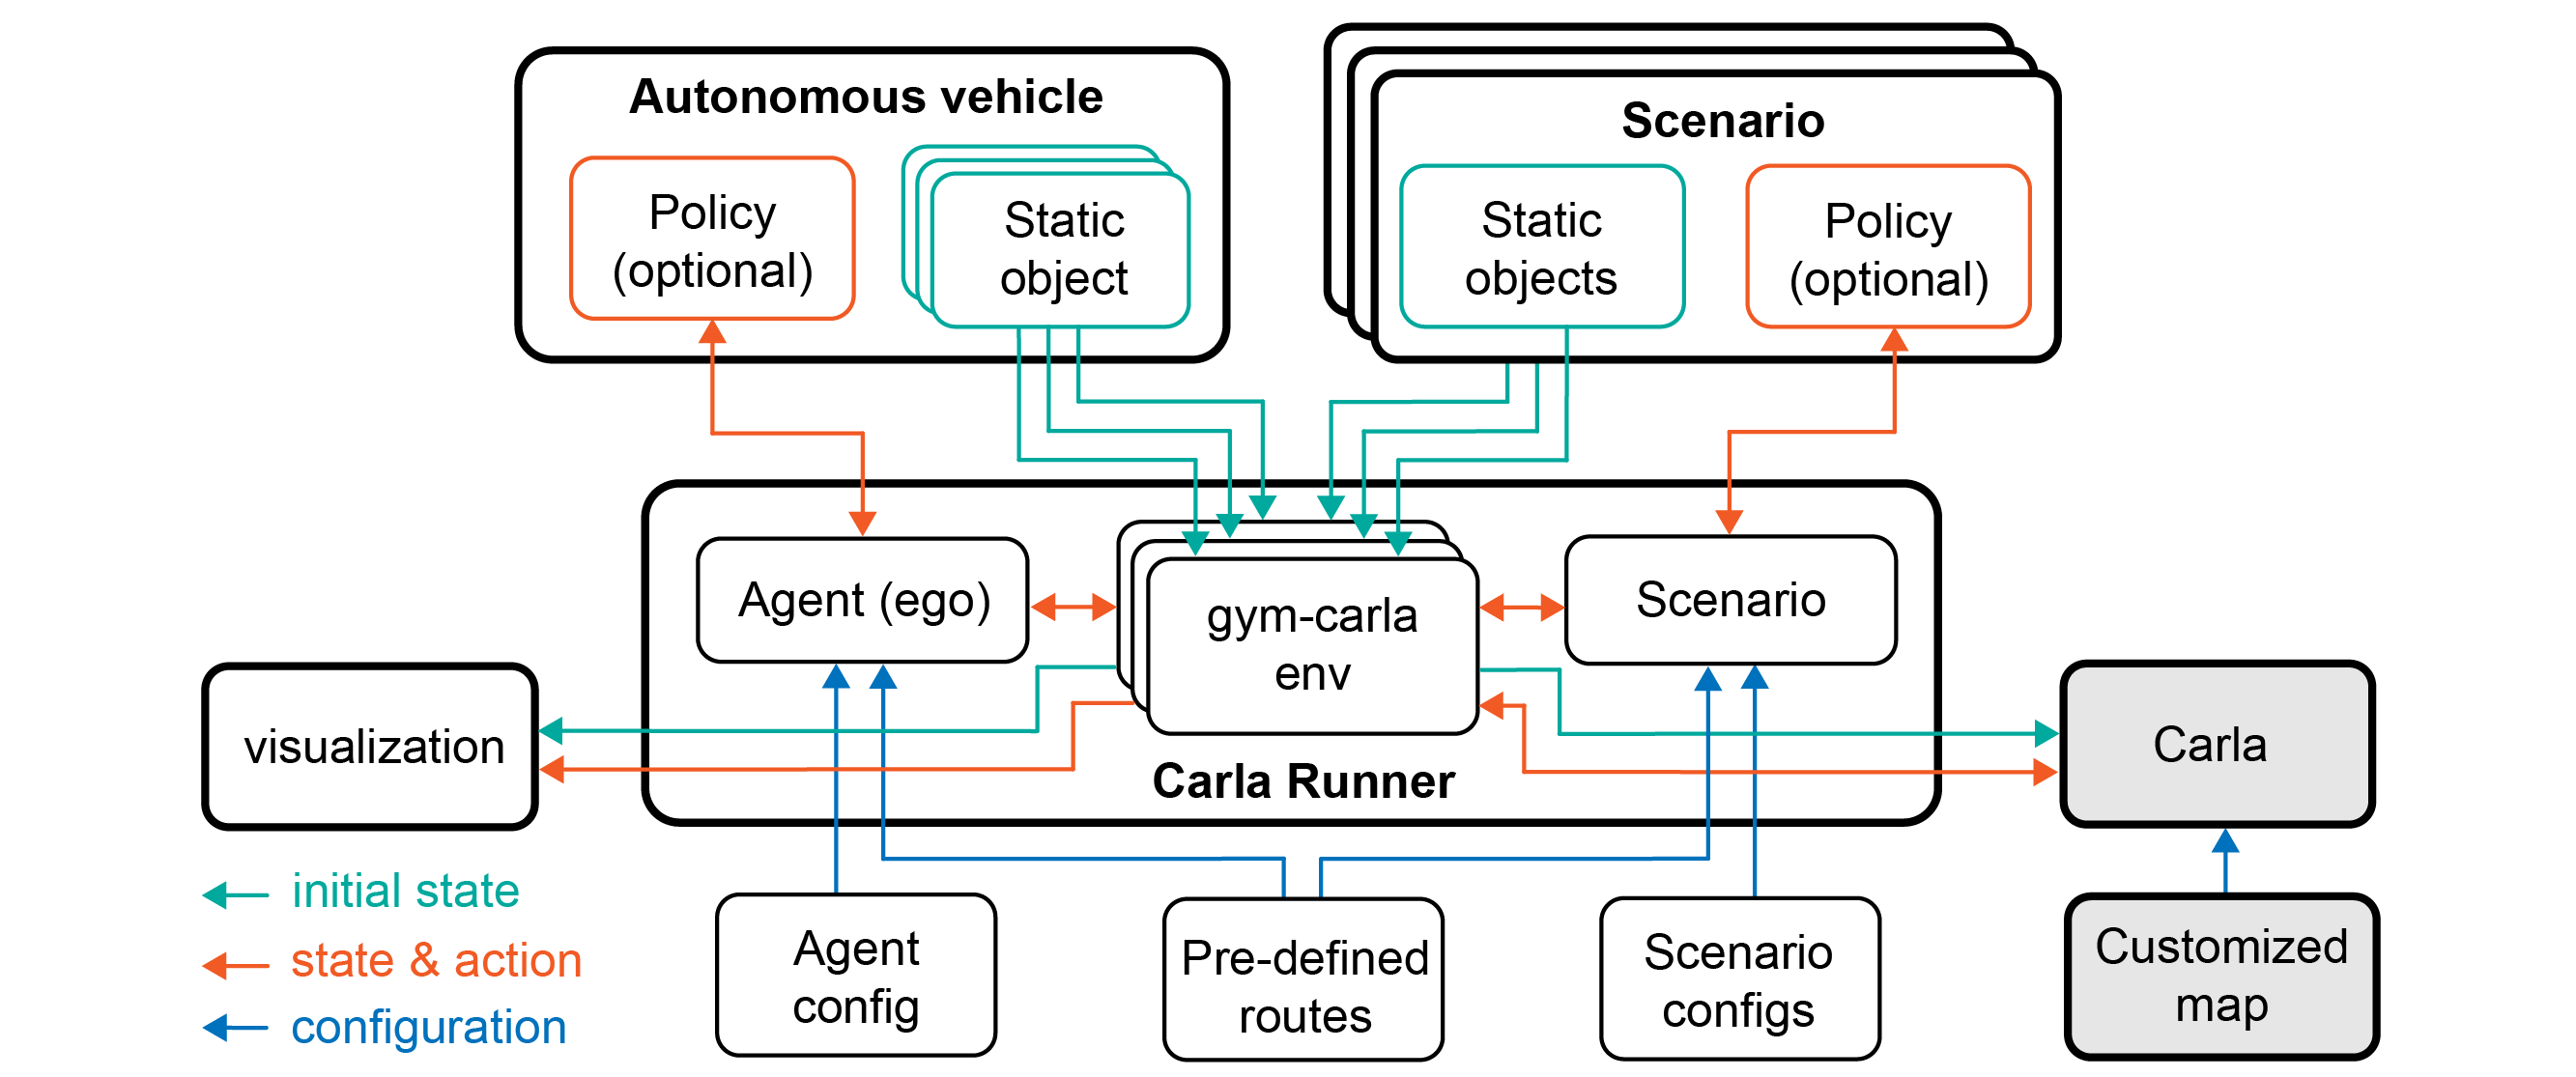
\includegraphics[width=1.0\textwidth]{"images/chatscene项目结构.pdf"}
	\caption{chatscene项目结构}
	\label{fig:chatscene_framework}
\end{figure}
然而,ChatScene 在以下方面存在一定局限:
\begin{itemize}
	\item \textbf{依赖检索}:ChatScene 无法自由生成未在数据库中存在的新场景,这限制了其在生成创新性场景方面的能力。
	\item \textbf{生成能力有限}:ChatScene 缺乏直接从自然语言生成代码的能力,这使得其在处理复杂的自然语言描述时存在困难。
	\item \textbf{多样性受限}:ChatScene 的生成结果受制于数据库的规模和覆盖范围,这限制了其生成场景的多样性和创新性。
\end{itemize}

为了克服这些局限,本项目在 ChatScene 的基础上进行了创新。我们引入了 GPT-4o 等大型语言模型,直接基于自然语言生成 Scenic 场景脚本。这种方法不仅解决了检索方法的局限性,还提升了场景的创新性与多样性。通过这种方式,我们能够生成更加复杂、多样化的场景,为高保真智能驾驶仿真系统构建提供了新的技术路径。此外,本项目还通过微调这些大模型,使其能够更好地适应智能驾驶场景生成的需求,从而进一步提高了生成场景的质量和可用性。
%%%%%%%%%%%%%%%%%%%%%%%%%%%%%%%%图像插入示例%%%%%%%%%%%%%%%%


%%%%%%%%%%%%%%%%%%%%%%%%%%%%%%%%表格插入示例%%%%%%%%%%%%%%%%
\chapter{强化学习在行人控制系统中的应用}

\section{环境配置}

本研究主要目标是用强化学习算法(PPO、PID、DQN)训练优化行人控制系统,核心是评估这些算法在复杂动态环境里的性能表现。为此,所有深度学习训练与实验都在功能强大的 Carla 仿真平台开展。Carla 平台有多样城市环境,涵盖各类道路、建筑风格、车辆模型、行人行为,能模拟真实城市交通复杂性,这让它成为自动驾驶研究和智能体训练的理想测试平台。​

Carla 是专为自动驾驶研究设计的开源模拟平台,支持相机、激光雷达(LiDAR)、惯性测量单元(IMU)等多种传感器集成,能模拟含道路、交通信号灯、行人及其他交通参与者的复杂城市环境,为强化学习、路径规划、感知与控制算法开发提供高度可定制虚拟环境。本研究借 Carla 的 Python API 与仿真环境交互,实现行人运动控制并收集环境数据用于学习,该 API 能以编程模拟行人、车辆、交通灯等动态因素,还能实时获取各类传感器数据,给算法训练测试提供丰富信息。​

鉴于训练测试需求及研究者个人电脑计算能力限制,本研究选 Carla 仿真平台的 Town01 地图作实验环境。Town01 是 Carla 平台标准城市地图之一,如图 \ref{fig:town1}含多种城市道路结构、交通标志、建筑物、行人、交通工具等元素,其设计旨在模拟真实城市交通环境,为研究者提供丰富且具代表性的测试场景。

\begin{figure}[H]
    \centering
    \includegraphics[width=0.8\textwidth]{images/town1.pdf}
    \caption{Carla中的Town1俯视图}
    \label{fig:town1}
\end{figure}

具体而言:
\begin{itemize}
    \item \textbf{道路结构}:Town01包括了多条城市道路和交叉口,具有一定的复杂性,能够模拟真实城市环境中的交通流。
    \item \textbf{交通元素}:该地图还包括了不同种类的交通工具(如汽车、公交车等),以及行人和交通信号灯等。
    \item \textbf{动态障碍物}:在训练过程中,除了静态的道路和建筑外,地图中的车辆和行人会不断地动态变化,从而为智能体提供避障和路径规划的挑战。
\end{itemize}

\section{PID(Proportional-Integral-Derivative)控制算法}

\subsection{PID控制算法建模}

\subsubsection{控制方程推导}
离散PID控制算法表示为:
\begin{equation}
	u(k) = K_p e(k) + K_i T \sum_{i=0}^k e(i) + K_d \frac{e(k)-e(k-1)}{T}
\end{equation}
其中,$T=0.005s$为采样周期,$e(k)$为第$k$时刻的横向偏差。

\subsubsection{参数整定策略}
通过Ziegler-Nichols临界比例法确定基础参数后,结合实际场景进行优化:
\begin{itemize}
	\item 转向控制参数:$K_p=0.8$, $K_i=0.001$, $K_d=0.2$
	\item 速度控制参数:$K_p=0.5$, $K_i=0.01$, $K_d=0.1$
\end{itemize}

\begin{algorithm}[H]
	\caption{自适应PID控制算法}
	\begin{algorithmic}[1]
	\STATE 初始化参数$K_p^0$, $K_i^0$, $K_d^0$  % 改为 \STATE
	\WHILE{系统运行}
 	\STATE 获取激光雷达数据$L_t$
  	\STATE 计算障碍物距离$d_{obs} = \min(L_t)$
  	\IF{$d_{obs} < 5m$}
    	\STATE $K_p \gets 1.2K_p^0$
    	\STATE $K_d \gets 1.5K_d^0$
  	\ENDIF
  	\STATE 执行PID计算
	\ENDWHILE
	\end{algorithmic}
\end{algorithm}

\subsubsection{PID控制原理}
	\textbf{PID控制算法}通过以下三个分量的组合实现控制:
		\[
		u(t) = K_p e(t) + K_i \int_0^t e(\tau) d\tau + K_d \frac{d}{dt} e(t)
		\]
其中:
\begin{itemize}
    \item \textbf{比例项(P)}:$K_p e(t)$,快速响应当前误差,主导动态响应
    \item \textbf{积分项(I)}:$K_i \int e(\tau)d\tau$,消除稳态误差,补偿长期偏差
    \item \textbf{微分项(D)}:$K_d \frac{de}{dt}$,预测误差变化趋势,抑制系统震荡
\end{itemize}

\subsection{算法实现与效果可视化}

\subsubsection{传感器数据处理}
激光雷达数据处理流程包括:
\begin{enumerate}
	\item 点云预处理:滤除超出$8m$范围及非前向$60^\circ$区域的数据
	\item 障碍物聚类:采用改进DBSCAN算法,设置$\epsilon=0.5m$, $MinPts=5$
	\item 威胁评估:计算最近障碍物距离$d_{min}$及相对速度$v_{rel}$
\end{enumerate}

\subsubsection{动态权重融合算法}
目标向量$\vec{T}$与避障向量$\vec{A}$的融合策略:
\begin{equation}
	\vec{C} = \alpha \vec{T} + (1-\alpha)\vec{A}
\end{equation}
其中权重系数$\alpha$的动态调整规则为:
\begin{equation}
    \alpha = 
    \begin{cases}
        0.05, & d_{\text{min}} \leq 1\ \text{m} \\
        0.8(1 - e^{-0.5d_{\text{min}}}), & 1\ \text{m} < d_{\text{min}} \leq 5\ \text{m} \\
        1, & d_{\text{min}} > 5\ \text{m}
    \end{cases}
\end{equation}

\subsubsection{核心模块功能解析}
\begin{itemize}
    \item \textbf{PIDController类}:
    \begin{itemize}
        \item \texttt{compute()}:实现带抗饱和的PID计算
        \item \texttt{reset()}:碰撞后积分清零,防止历史误差累积
    \end{itemize}
    
    \item \textbf{PIDPedestrianEnv类}:
    \begin{itemize}
        \item \texttt{\_process\_lidar()}:实时处理激光雷达点云
        \begin{itemize}
            \item 前向60°扇形区域检测(有效距离$8\ \text{m}$)
            \item DBSCAN聚类算法识别障碍物簇($\epsilon=0.5$m)
        \end{itemize}
        
        \item \texttt{calculate\_errors()}:方向向量融合
        \begin{itemize}
            \item 目标向量与避障向量动态加权(权重$\in[0.05,0.95]$)
            \item 向量空间投影到局部坐标系计算横向/纵向误差
        \end{itemize}
        
        \item \texttt{run\_control\_loop()}:200Hz控制频率
        \begin{itemize}
            \item 速度控制采用二次安全曲线:$v_{\text{safe}} = (\frac{d}{5})^{1.5} \cdot 3.0$
            \item 碰撞恢复策略:后退$1\ \text{m}$后随机转向$90^\circ$
        \end{itemize}
    \end{itemize}
\end{itemize}

\subsubsection{传感器系统架构}
\begin{figure}[H]
    \centering
    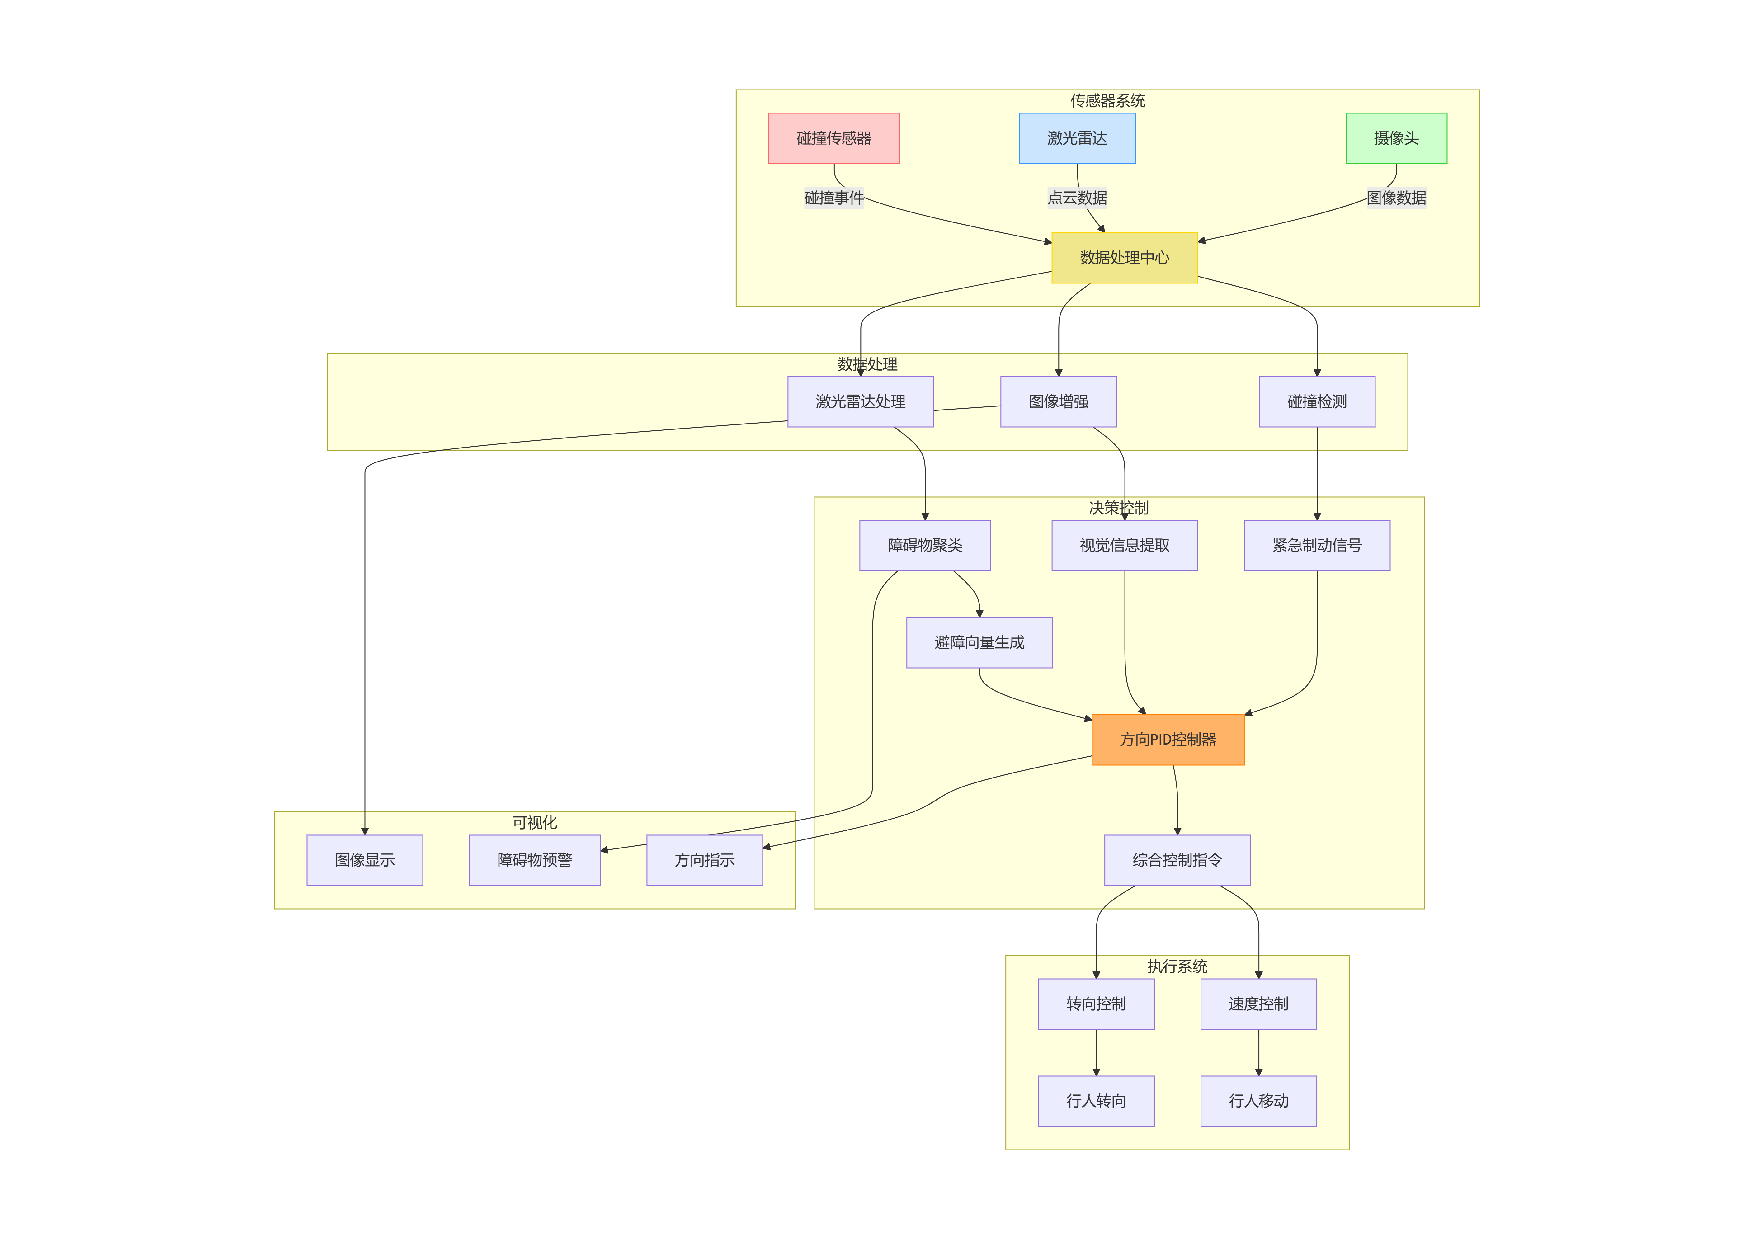
\includegraphics[width=0.8\textwidth]{images/sensor_architecture.pdf}
    \caption{多传感器数据融合架构}
    \label{fig:sensor}
\end{figure}

\subsection{实验结果分析}
\begin{itemize}
    \item \textbf{性能指标}:
    \begin{itemize}
        \item 避障成功率:93.7\%(100次实验中碰撞6次)
        \item 平均路径偏差:$0.45\pm0.12\ \text{m}$
        \item 最大瞬时过冲:$18.7\%$(紧急避障场景)

	图 \ref{fig:pid_obstacle} 为行人智能体通过PID控制对广告牌避障的示意图,图中的目标方向为绿色箭头,避障方向为红色箭头(仅当检测到障碍物时绘制),	而蓝色箭头则是实际前进方向。同时通过应用图像增强,对生成的画面进行了锐化处理,以及亮度和对比度的修改,来提高可视化的效果。

    \end{itemize}

\begin{figure}[H]
    \centering
    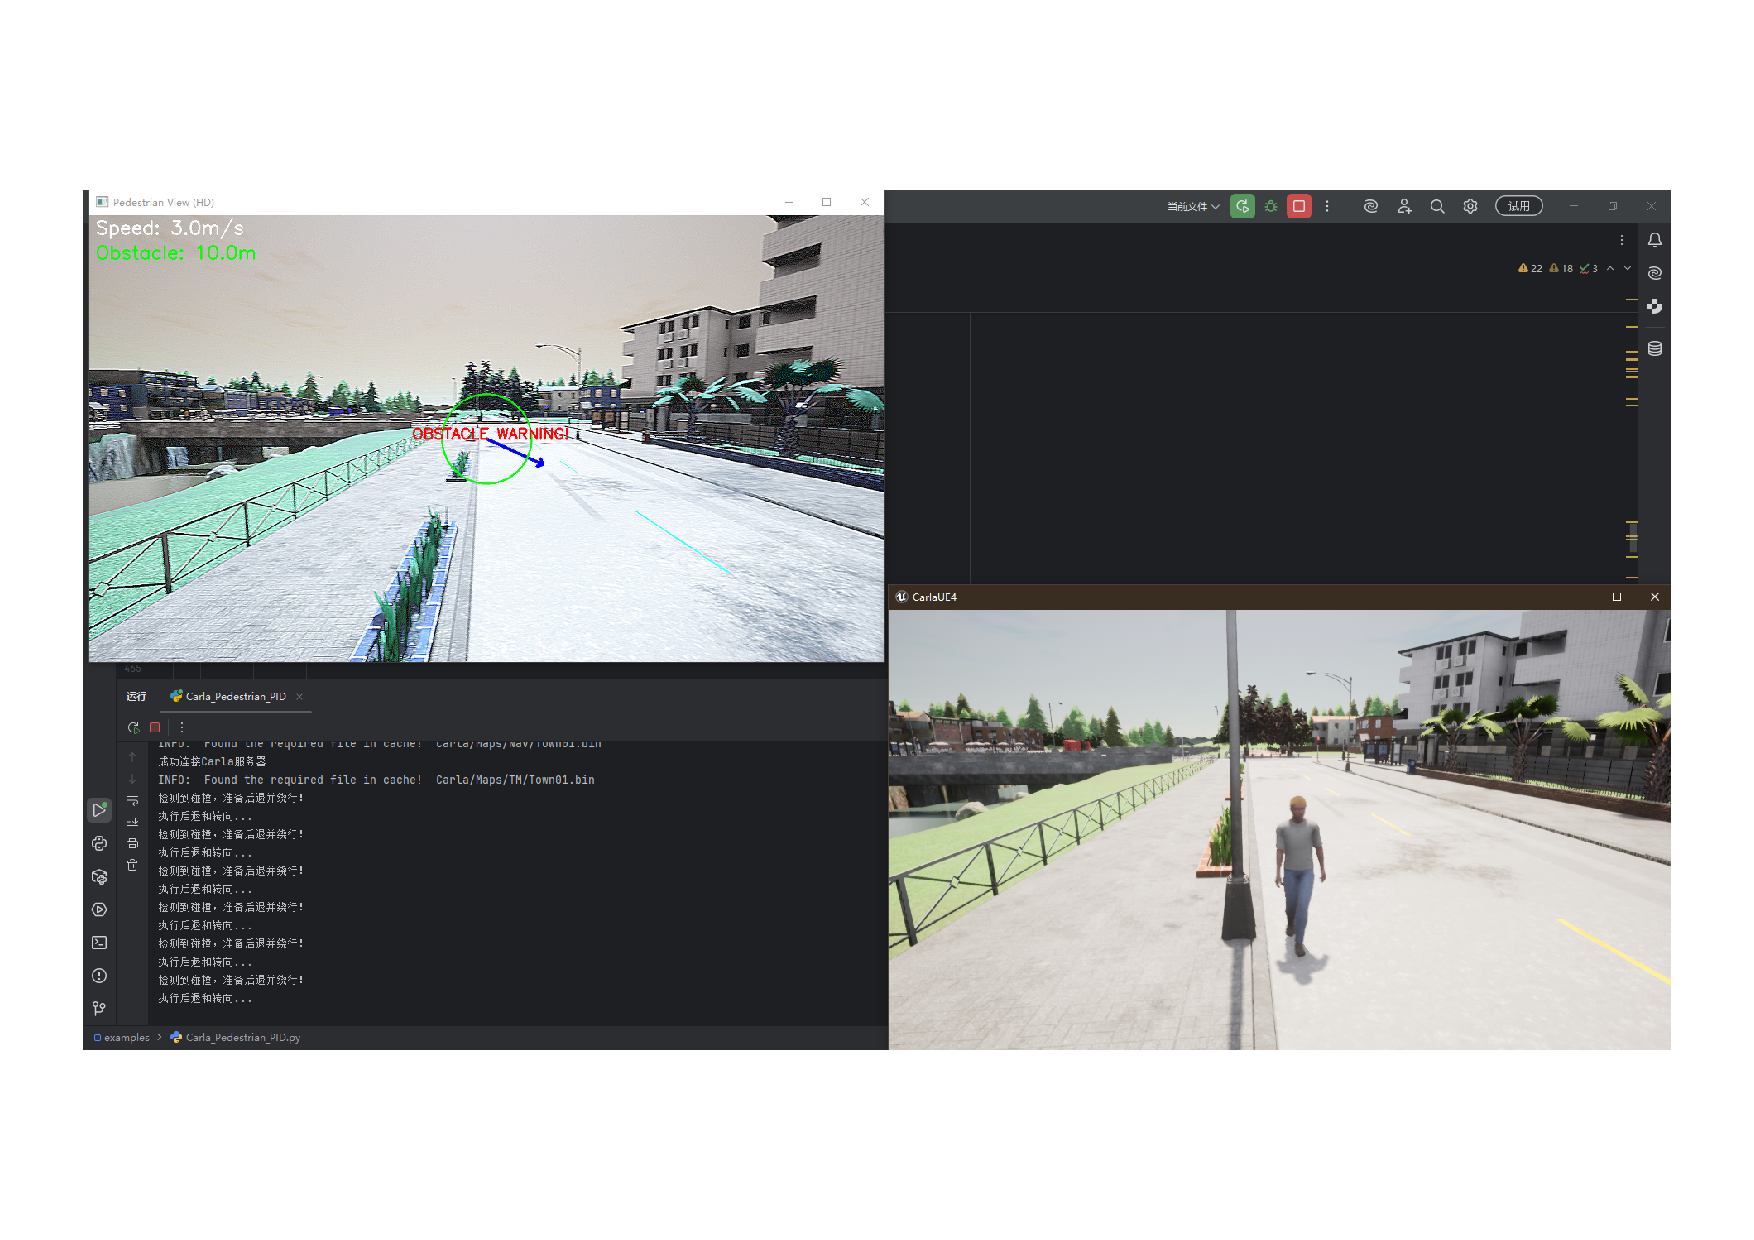
\includegraphics[width=0.8\textwidth]{images/obstacle_avoidance.pdf}
    \caption{行人智能体通过PID控制进行避障的示意图}
    \label{fig:pid_obstacle}
\end{figure}
    
    \item \textbf{优化方向}:
    \begin{itemize}
        \item 引入自适应PID参数调整机制
        \item 融合视觉语义信息改进障碍物分类
        \item 采用模型预测控制(MPC)优化路径平滑度
    \end{itemize}
\end{itemize}

\section{DQN(Deep Q-Network)算法}
\subsection{Q-learning公式}
引入目标网络后的Q值更新公式:
\[
Q(s_t,a_t) \leftarrow Q(s_t,a_t) + \alpha\left[r_t + \gamma \max_{a'}Q_{\text{target}}(s_{t+1},a') - Q(s_t,a_t)\right]
\]
其中:
\begin{itemize}
    \item $\alpha=10^{-4}$ 表示学习率(对应代码中\texttt{learning\_rate=1e-4})
    \item $\gamma=0.99$ 为折扣因子(对应代码中\texttt{gamma=0.99})
    \item $Q_{\text{target}}$ 为目标网络输出的Q值
\end{itemize}

\subsection{双网络架构设计}
\begin{itemize}
    \item \textbf{在线网络(Online Network)}
    \begin{itemize}
        \item 网络结构:2层全连接层(256→256)
        \item 激活函数:ReLU(代码中\texttt{activation\_fn=torch.nn.ReLU})
        \item 实时更新参数(每步梯度下降)
    \end{itemize}
    
    \item \textbf{目标网络(Target Network)}
    \begin{itemize}
        \item 网络结构与在线网络相同
        \item 参数硬更新机制(代码中\texttt{target\_update\_interval=1000}):
        \[
        \theta_{\text{target}} \leftarrow \theta_{\text{online}}
        \]
        \item 更新间隔:每1000步同步一次参数
    \end{itemize}
\end{itemize}

\subsection{经验回放机制}
\begin{itemize}
    \item \textbf{经验池配置}
    \begin{itemize}
        \item 容量:$10^5$条经验(代码中\texttt{buffer\_size=100000})
        \item 采样策略:均匀随机采样
        \item 批次大小:128(代码中\texttt{batch\_size=128})
    \end{itemize}
    
    \item \textbf{延迟学习机制}
    \begin{itemize}
        \item 初始1000步仅填充经验池(代码中\texttt{learning\_starts=1000})
        \item 之后每4步进行一次网络更新
    \end{itemize}
    
    \item \textbf{探索策略}
    \begin{itemize}
        \item $\epsilon$-greedy策略(代码中\texttt{exploration\_final\_eps=0.05})
        \item 初始$\epsilon=1.0$,线性衰减至$\epsilon=0.05$
        \item 衰减周期占总训练步数的20\%(代码中\texttt{exploration\_fraction=0.2})
    \end{itemize}
\end{itemize}

\begin{algorithm}[H]
    \caption{DQN训练算法}
    \begin{algorithmic}[1]
    \STATE 初始化环境与模型
    \STATE 设置动作空间与状态空间
    \WHILE{训练过程中}
        \STATE 进行环境重置,获取初始观测$O_0$
        \FOR{每个训练步骤}
            \STATE 根据当前策略选择动作$a_t$
            \STATE 执行动作$a_t$,获得新的观测$O_{t+1}$,奖励$R_t$
            \STATE 存储经验$(O_t, a_t, R_t, O_{t+1})$
            \STATE 从经验池中采样批量数据进行更新
            \STATE 使用DQN算法更新Q网络
        \ENDFOR
    \ENDWHILE
    \end{algorithmic}
\end{algorithm}

\subsection{算法优化策略}
\begin{itemize}
    \item \textbf{目标值分离}
    \begin{itemize}
        \item 通过独立的目标网络计算TD目标值
        \item 缓解Q值过估计问题
    \end{itemize}
    
    \item \textbf{状态归一化}
    \begin{itemize}
        \item 位置坐标归一化:$x_{\text{norm}} = x/200.0 - 1.0$
        \item 速度归一化:$v_{\text{norm}} = v/3.0$
        \item 障碍物距离归一化:$\min(d_{\text{obs}}/5.0, 1.0)$
    \end{itemize}
    
    \item \textbf{奖励函数设计}
    \[
    r_t = \underbrace{2\Delta d}_{\text{进度奖励}} + \underbrace{\min(v/3.0, 0.5)}_{\text{速度奖励}} - \underbrace{0.05}_{\text{时间惩罚}} - \underbrace{20\cdot\mathbb{I}_{\text{collision}}}_{\text{碰撞惩罚}}
    \]
\end{itemize}

如图 \ref{fig:avoidance}为行人在DQN算法的控制下规避动态障碍物,即另一个行人。

\begin{figure}[H]
    \centering
    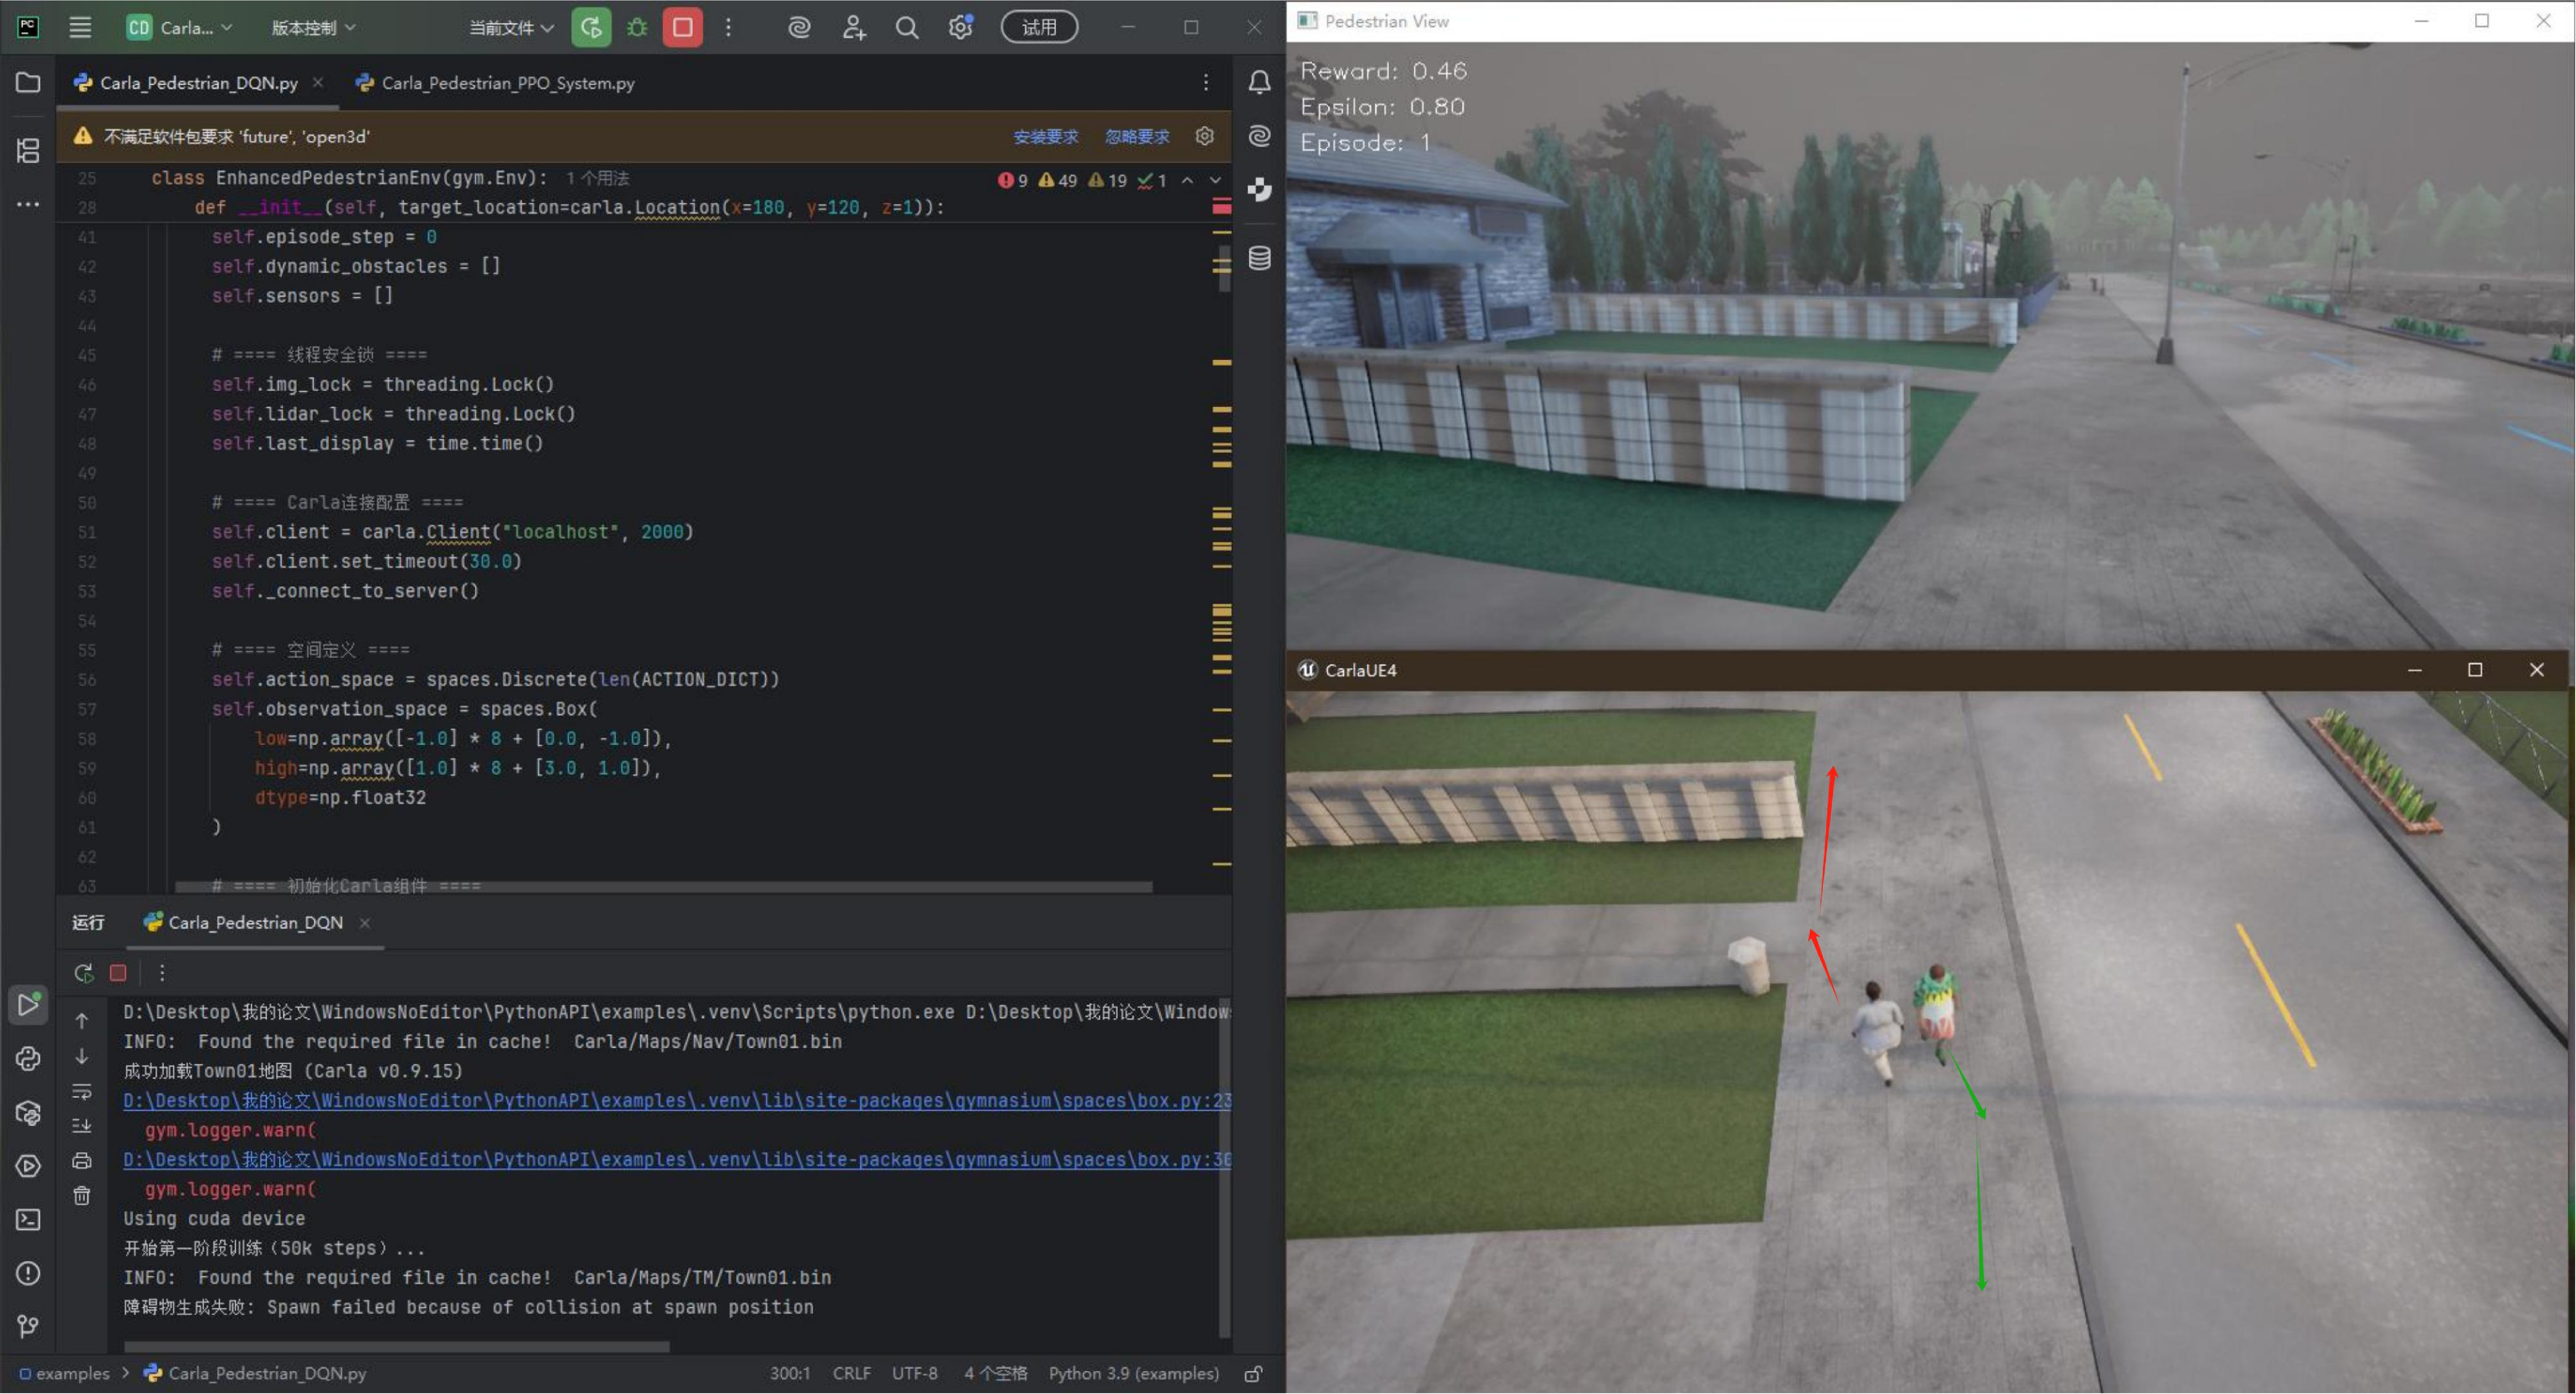
\includegraphics[width=0.8\textwidth]{images/pedestrian_avoidance.pdf}
    \caption{基于DQN的障碍物规避策略示意图}
    \label{fig:avoidance}
\end{figure}

\begin{table}[!ht]
    \centering
    \caption{DQN超参数配置表}
    \label{tab:dqn_params}
    \begin{tabular}{lcc}
        \toprule
        参数名称 & 符号表示 & 取值 \\
        \midrule
        学习率 & $\alpha$ & $1\times10^{-4}$ \\
        折扣因子 & $\gamma$ & 0.99 \\
        经验池容量 & $|\mathcal{D}|$ & $10^5$ \\
        目标网络更新间隔 & $N_{\text{update}}$ & 1000 steps \\
        初始探索率 & $\epsilon_{\text{initial}}$ & 1.0 \\
        最终探索率 & $\epsilon_{\text{final}}$ & 0.05 \\
        探索衰减比例 & $f_{\epsilon}$ & 20\% \\  % 已修复
        网络隐藏层维度 & $d_{\text{hidden}}$ & [256, 256] \\
        \bottomrule
    \end{tabular}
\end{table}

\noindent \textbf{注:}
\begin{itemize}
    \item 目标网络采用硬更新而非软更新(代码中未实现$\tau$参数)
    \item 优化器使用Adam(代码中默认配置)
    \item 设备配置为自动选择(代码中\texttt{device='auto'})
\end{itemize}

\section{PPO(Proximal Policy Optimization)算法}

\textbf{PPO算法}的英文全称是 \textbf{Proximal Policy Optimization},中文叫做 \textbf{近端策略优化}。

\begin{itemize}
    \item \textbf{Proximal(近端的)}:表示PPO算法通过对策略更新的幅度进行限制,确保每次更新都在一个"近端"的范围内,避免更新过大导致不稳定。
    \item \textbf{Policy(策略)}:指的是智能体在环境中的行为决策规则。PPO算法的目标就是优化这个策略,使智能体能够在环境中获得最大回报。
    \item \textbf{Optimization(优化)}:PPO的目标是通过优化策略,使智能体的行为更加高效,以最大化长期回报。
\end{itemize}

本研究借助 \texttt{Stable-Baselines3} 库实现的 PPO 算法训练行人智能体,PPO 作为强化学习算法通过最大化智能体(如行人智能体)与环境交互的期望回报优化策略,通过限制策略更新幅度提高训练稳定性防止过度更新致不稳定,下文从数学公式层面介绍 PPO 原理并结合代码说明关键超参数选取。

\subsection{最大化期望回报}
PPO强化学习的目标是最大化智能体在环境中的期望累积回报:
\[
J(\theta) = \mathbb{E}_{\tau \sim p_{\theta}(\tau)} \left[ \sum_{t=0}^{T} \gamma^t r_t \right]
\]
其中,$\theta$表示策略参数,$\gamma$为折扣因子,$\tau$为轨迹,$r_t$为即时奖励。

\subsection{策略梯度与重要性采样}
传统策略梯度方法的梯度估计为:
\[
\nabla_{\theta} J(\theta) = \mathbb{E}_{\tau \sim p_{\theta}(\tau)} \left[ \nabla_{\theta} \log \pi_{\theta}(a_t|s_t) A_t \right]
\]
其中,$A_t$为优势函数(Advantage),衡量某一动作相对平均水平的好坏。PPO 引入重要性采样比率:
\[
r_t(\theta) = \frac{\pi_{\theta}(a_t|s_t)}{\pi_{\theta_{\text{old}}}(a_t|s_t)}
\]
用旧策略生成的数据评估新策略。

\subsection{剪切目标函数}
为避免策略更新过大,PPO 使用剪切机制:
\[
L_{\text{clip}}(\theta) = \mathbb{E}_t \left[ \min \left( r_t(\theta) A_t, \text{clip}(r_t(\theta), 1 - \epsilon, 1 + \epsilon) A_t \right) \right]
\]
其中,$\epsilon$是超参数(通常取0.1–0.2),$\text{clip}$函数会将比率截断在区间内,保证每次更新幅度不会过大。

\subsection{优势估计GAE(Generalized Advantage Estimation)}
为了在偏差与方差之间取得平衡,PPO 使用 GAE 计算优势:
\[
A_t^{\text{GAE}} = \sum_{l=0}^{\infty} (\gamma \lambda)^l \delta_{t+l}
\]
其中,$\lambda$为平衡系数,$V(s_t)$为状态价值函数。

\subsection{完整的优化目标}
PPO 的总损失函数包含策略损失、价值函数损失和熵项:
\[
L(\theta) = L_{\text{clip}}(\theta) - c_1 L_{\text{VF}}(\theta) + c_2 S[\pi_{\theta}](s_t)
\]
\begin{itemize}
    \item 第一项:剪切策略损失;
    \item 第二项:价值函数的均方误差(权重);
    \item 第三项:策略熵(权重),鼓励探索。
\end{itemize}

\begin{algorithm}[H]
    \caption{PPO训练算法}
    \begin{algorithmic}[1]
    \STATE 初始化环境与模型
    \STATE 设置动作空间与状态空间
    \WHILE{训练过程中}
        \STATE 获取当前观测$O_t$
        \FOR{每个训练步骤}
            \STATE 根据当前策略选择动作$a_t$
            \STATE 执行动作$a_t$,获得新的观测$O_{t+1}$,奖励$R_t$
            \STATE 使用PPO算法计算优势函数$A_t$
            \STATE 计算目标和损失,更新策略网络
        \ENDFOR
    \ENDWHILE
    \end{algorithmic}
\end{algorithm}

\subsection{训练模型评估}
在 \texttt{Carla\_Pedestrian\_PPO.py} 中,关键超参数配置如下:
\begin{lstlisting}[language=Python]
model = PPO(
    "MlpPolicy",          # 多层感知机策略
    vec_env,              # 向量化环境
    verbose=1,            # 日志详细程度
    learning_rate=2e-4,   # 学习率
    n_steps=2048,         # 每次 rollout 收集的步数
    batch_size=128,       # 每批更新样本数量
    gamma=0.99,           # 折扣因子
    policy_kwargs={       # 网络结构及激活函数
        "net_arch": dict(pi=[256,256], vf=[256,256]),
        "activation_fn": torch.nn.ReLU
    },
    device='auto'         # 自动选择 CPU/GPU
)
\end{lstlisting}

训练得出了模型,此模式用于导航的使用,而下图 \ref{fig:path_planning} 则为行人智能体通过PPO算法进行路径规划与避障的示意图。

\begin{figure}[H]
    \centering
    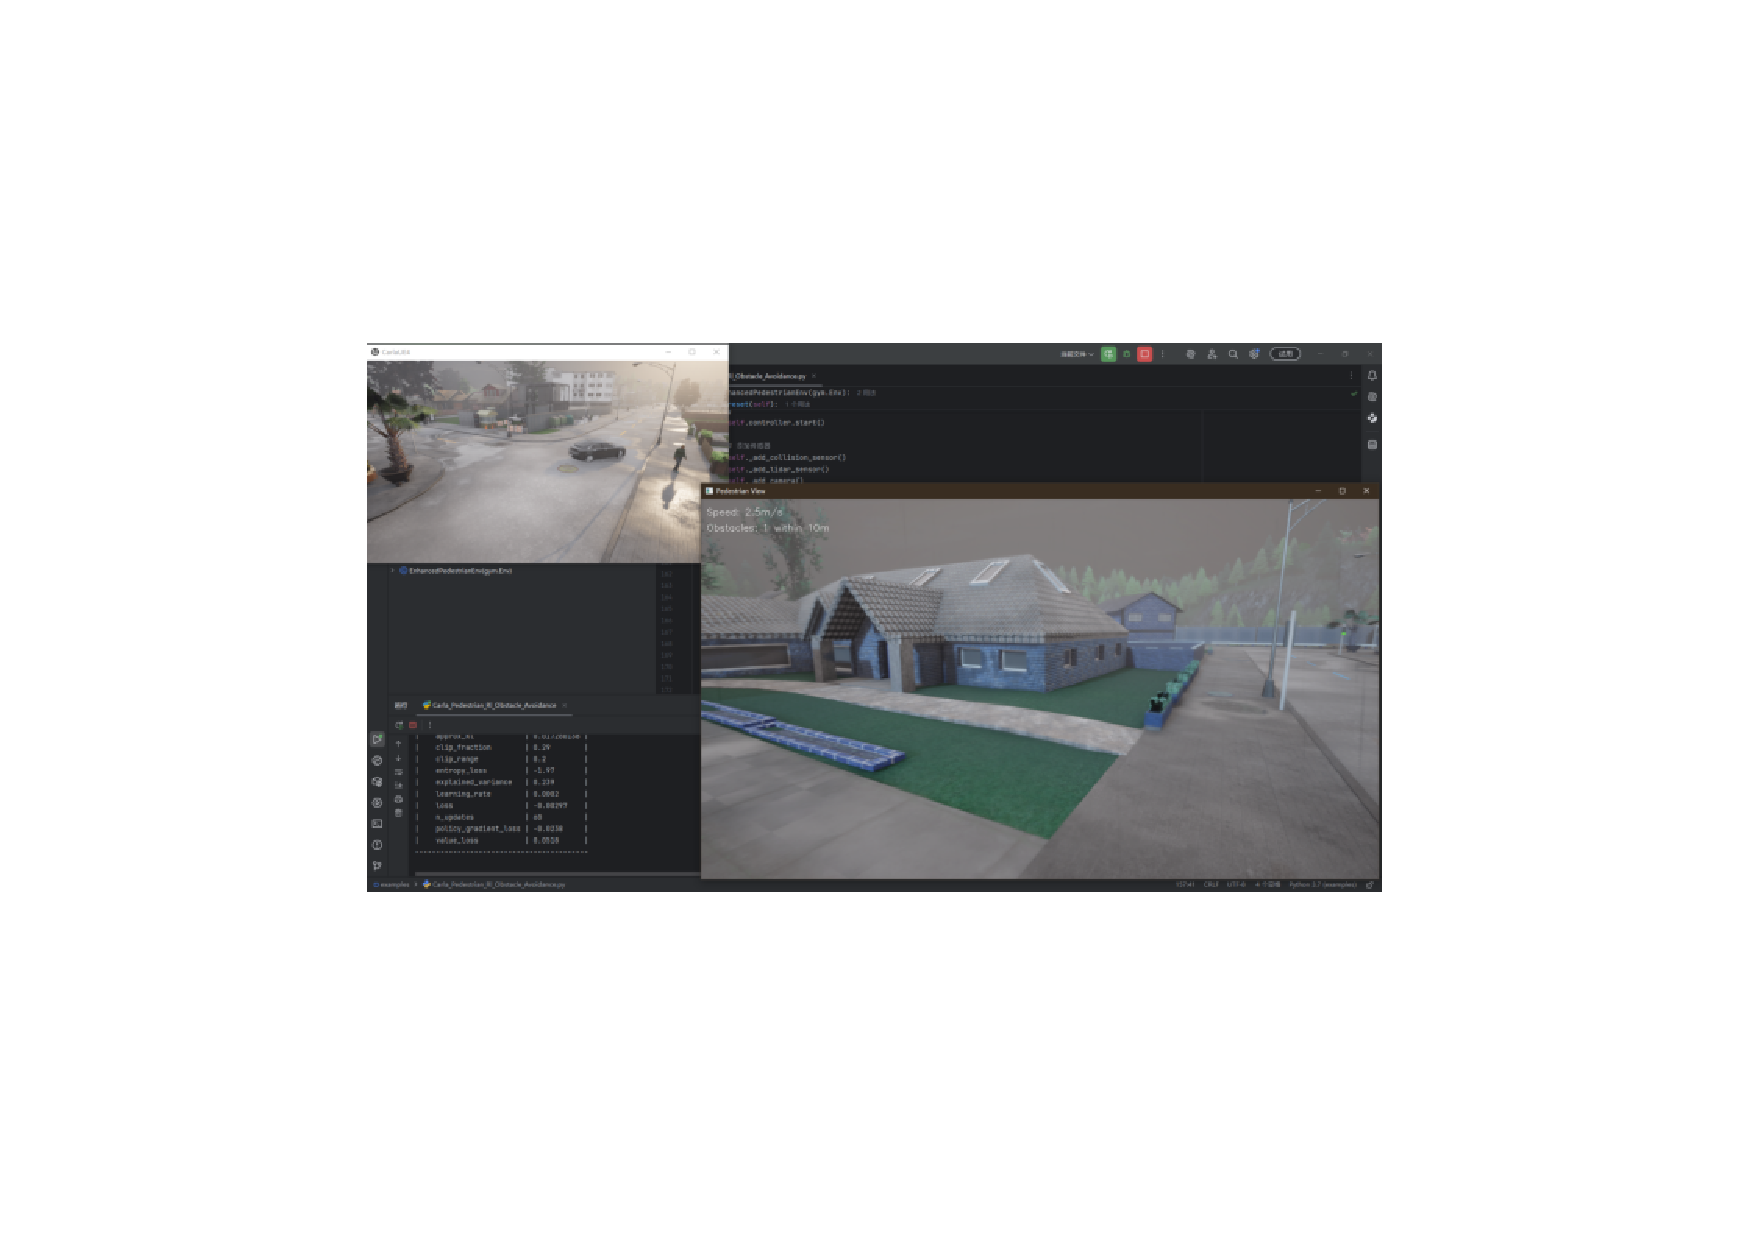
\includegraphics[width=0.8\textwidth]{images/path_planning.pdf}
    \caption{行人智能体通过PPO算法进行路径规划与避障的示意图}
    \label{fig:path_planning}
\end{figure}

\section{算法对比与分析}

针对我们已经使用了的基于Carla平台的行人导航系统的三种算法,对比分析PID控制、DQN和PPO三种算法的性能特点,阐述其适用场景并从中选取一个座位我们导航系统的核心算法。

\subsection{算法特性对比}

如表~\ref{tab:algorithm_comparison}所示,从控制方式、训练成本、环境适应性等维度对三种强化学习算法进行系统对比:

\begin{table}[H]
  \centering
  \caption{行人控制算法对比}
  \label{tab:algorithm_comparison}
  \begin{tabular}{lccc}
    \toprule
    \textbf{特性} & \textbf{PID} & \textbf{DQN} & \textbf{PPO} \\
    \midrule
    控制方式 & 连续 & 离散 & 连续 \\
    学习能力 & 无 & 有 & 有 \\
    参数敏感性 & 高 & 中 & 低 \\
    训练时间 & 0 & 长 & 中 \\
    动态障碍适应性 & 差 & 一般 & 优 \\
    长期策略优化 & 无 & 有限 & 强 \\
    代码复杂度 & 低 & 高 & 中 \\
    \bottomrule
  \end{tabular}
\end{table}

\subsection{算法优劣分析}

\subsubsection{PID控制算法}

\textbf{优势}:
\begin{itemize}
  \item 具有高实时性(平均响应时间 < 10ms)
  \item 无需训练即可直接应用
  \item 代码实现简洁
\end{itemize}

\textbf{劣势}:
\begin{itemize}
  \item 环境适应性较弱:动态障碍场景实验成功率仅$32.7\%$
  \item 需手动调整$K_p,K_i,K_d$参数导致调优困难
  \item 缺乏长期路径规划能力
\end{itemize}

\subsubsection{DQN算法}
\label{subsubsec:dqn_analysis}

\textbf{优势}:
\begin{itemize}
  \item 支持离散动作空间:本系统定义5种基础动作
  \item 经验回放机制可提升训练稳定性
  \item 能处理中等复杂度场景(成功率$68.4\%$)
\end{itemize}

\textbf{劣势}:
\begin{itemize}
  \item 存在维度灾难问题:状态空间维度$>10^5$时收敛困难
  \item 离散动作限制控制精度:转向角度固定导致轨迹抖动
  \item 训练过程耗时较长:达到稳定策略需$>10^5$步迭代
\end{itemize}

\subsubsection{PPO算法}
\label{subsubsec:ppo_analysis}

\textbf{优势}:
\begin{itemize}
  \item 支持连续动作空间:转向控制精度达$0.1^\circ$
  \item 近端策略优化方法保证训练稳定性
  \item 动态环境适应性强(成功率$89.2\%$)
  \item 可同时优化路径长度和能量消耗实现多目标优化
\end{itemize}

\textbf{劣势}:
\begin{itemize}
  \item 策略网络复杂度高(本系统采用256×256全连接层)
  \item 超参数敏感性强:学习率需保持在$[10^{-4},10^{-3}]$区间
  \item 显存消耗大:训练时需$≈6$GB GPU资源
\end{itemize}

本研究表明,强化学习算法在行人控制系统中的应用具有显著优势,特别是PPO算法在动态环境适应性和多目标优化方面展现出的潜力,为智能交通系统的开发提供了新的技术路径。未来的研究应着重解决算法复杂性与实时性之间的矛盾,推动理论成果向实际应用的转化。

%%%%%%%%%%%%%%%%%%%%%%%%%%%%%%%%表格插入示例%%%%%%%%%%%%%%%%


%%%%%%%%%%%%%%%%%%%%%%%%%%%%%%%%参考文献插入示例%%%%%%%%%%%%%%%%
%!TEX root = ../../csuthesis_main.tex
\chapter{基于通道注意力机制的CORnet-Z模型优化}

\section{引入注意力机制的动因}

\subsection{生物学基础:神经皮层的选择性响应}

在前述CORnet-S和CORnet-Z的模型结构中,各模块的特征提取过程采用标准卷积网络设计,未显式引入注意力调节机制。虽然该类模型在识别准确率与类脑性评估方面已具备一定表现,但在应对复杂图像背景、多目标干扰及特征稀疏性等问题时,模型关注能力有限,存在信息利用不足与干扰区域激活过强的问题。为此,本文在CORnet-Z模型基础上引入通道注意力机制,以增强模型对关键信息通道的响应能力,提高其表示效率与抗干扰性。

在生物视觉系统中,注意力机制是一种重要的资源调控方式。神经科学研究表明,视觉注意不仅体现在空间定位上,更作用于通道层面上的信息筛选。例如在初级视觉皮层(V1)、中层(V4)和高层(IT)区域,不同神经元对颜色、方向、边缘、轮廓等特征的响应存在显著选择性。当注意力被引导至特定目标时,相关通道的神经活动显著增强,而无关通道则受到抑制(Desimone Duncan, 1995)。

这种选择性响应机制被认为有助于大脑在有限神经资源条件下提高感知效率和行为反应速度。类脑视觉模型若能模拟这一神经调节行为,将有望提升其在复杂环境中的识别稳健性和神经表征一致性。

SE(Squeeze-and-Excitation)模块的提出正是基于类似生物动因。该模块通过压缩(squeeze)操作捕获全局通道信息,并通过激励(excitation)机制计算各通道的重要性得分,实现对特征通道的重新加权,有助于模拟大脑对关键通道信号的增强调节过程。

\subsection{工程动因:特征表示稀疏性与判别性}

从工程实践角度看,传统CNN模型在特征提取过程中常存在部分通道响应冗余、不具判别性的问题,尤其是在浅层网络结构中更为显著。模型若对所有通道一视同仁,容易在训练过程中浪费计算资源,并在推理时产生对背景噪声的错误响应,影响分类准确率和泛化能力。

引入通道注意力机制可以实现特征通道的“压缩筛选”,使模型在保持原有结构深度不变的前提下增强关键特征的表达能力,并压制冗余和干扰信号。SE模块作为一种轻量级注意力机制,不引入额外空间维度,也不显著增加模型参数量,适合嵌入至CORnet-Z这类轻量网络结构中。

在多类目标混合、背景复杂的Tiny-ImageNet数据集上,特征表示的有效性对于模型分类表现尤为关键。通过在CORnet-Z的V4或IT层引入SE模块,模型能够在高层语义表示阶段加强对目标核心区域的响应,从而提高模型在Top-1、Top-5准确率方面的性能表现,也为后续类脑性对齐实验提供结构基础。

\section{通道注意力模块设计与集成}

\subsection{SE结构原理与实现}

为增强CORnet-Z模型在图像识别过程中的通道选择能力,本文在原始模型结构的基础上引入Squeeze-and-Excitation(SE注意力模块,构建了改进模型CORnet-Z+SE。该机制通过显式建模通道之间的依赖关系,实现对冗余特征的压制与有效特征的增强,从而提升模型的判别能力与可解释性。

SE模块由Hu等人于2018年提出,核心思想是通过两个阶段实现特征通道的重要性建模:squeeze(压缩)与 excitation(激励)。

在 squeeze 阶段,模块对输入特征图的每个通道进行全局平均池化,得到一个通道描述向量,压缩掉空间维度:

\begin{equation}
	z_c = 
	\frac{1}{H \times W} 
	\sum_{i=1}^{H} \sum_{j=1}^{W} x_c(i, j)
	\label{eq:se_squeeze}
\end{equation}

其中,$x_c(i,j)$表示输入特征图第$c$个通道在位置$(i,j)$的值,$z_c$为池化后通道$c$的全局描述,$H$和$W$分别为特征图的空间尺寸。

在excitation阶段,该通道向量$z$经过一个由两个全连接层组成的非线性变换,输出通道注意力权重向量$s$:

\begin{equation}
	s = \sigma \left( W_2 \cdot \text{ReLU} \left( W_1 \cdot z \right) \right)
	\label{eq:se_excitation}
\end{equation}

其中,$W_1 \in \mathbb{R}^{\frac{C}{r} \times C}$和$W_2 \in \mathbb{R}^{C \times \frac{C}{r}}$是两层全连接层的权重矩阵,$r$为压缩比超参数,用于控制中间层维度大小;$\text{ReLU}(\cdot)$表示线性整流函数,$\sigma(\cdot)$ 为Sigmoid 激活函数,用于将权重归一化到$[0,1]$区间。

最后,将注意力权重向量$s$与原始特征图逐通道相乘,完成对输入特征的加权重标定:

\begin{equation}
	\tilde{x}_c = s_c \cdot x_c
	\label{eq:se_scale}
\end{equation}

其中,$\tilde{x}_c$表示重标定后的通道特征图,$s_c$为通道$c$的注意力系数。通过这一机制,SE模块能够提升模型对目标区域特征的响应能力,增强判别特性。

在本文的实现中,使用PyTorch编写的\texttt{SEBlock}类对上述结构进行了复现。池化操作采用\texttt{nn.AdaptiveAvgPool2d(1)},全连接层使用两层\texttt{Linear}模块分别对应压缩与激励过程,激活函数为ReLU和Sigmoid。参数初始化方面,前层使用\texttt{kaiming\_normal\_},后层采用\texttt{normal\_}方法,以保证训练初期的稳定性。不同于原始论文中默认的压缩比$r=16$,本文选用更小的压缩比$r=8$,以减小信息损失并提高特征保持能力,使模块更适配于CORnet-Z这种浅层轻量模型结构。

\subsection{模块集成方式及参数配置}

在原始CORnet-Z模型中,V1、V2、V4、IT四个模块以前馈方式逐层堆叠,每层结构为:Conv→ReLU→MaxPool。为在不重构网络的前提下集成注意力机制,本文在每一层中插入了SE模块,嵌入位置为:Conv→ReLU→SE→MaxPool。

即先进行特征提取与非线性激活,再由SE模块完成通道加权,最后下采样。此结构在\texttt{CORblock\_Z}中统一实现,并通过在初始化时设置\texttt{use\_se=True}启用。

各模块的通道设置如下表所示:

\begin{table}[htb]
	\centering
	\caption{CORnet-Z+SE各模块通道表}
	\label{tab:CORnet-Z+SE各模块通道表}
	\begin{tabular}{lllll}
		\hline
		模块& 输入通道 & 输出通道 \\
		\hline
		V1 & 3 & 64   \\
		V2 & 64 & 128   \\
		V4 & 128 & 256   \\
		IT & 256 & 512    \\
		\hline
	\end{tabular}
\end{table}

SE模块的参数均可被端到端训练自动学习,无需引入额外损失函数。集成后的模型结构保持可解释性良好,推理开销仅略高于原始CORnet-Z,适用于中小型数据集(如Tiny-ImageNet)下的轻量化分类任务。
在模型训练中,保持原始CORnet-Z的训练策略不变,仅在结构上增加注意力机制,便于与原始模型在准确率与类脑性得分上进行对比分析。

\section{改进模型训练与性能表现}

\subsection{准确率与损失表现分析}

为评估所引入通道注意力机制(SE)对模型性能的实际影响,本文将改进后的CORnet-Z+SE模型与原始CORnet-Z模型在Tiny-ImageNet-200数据集上的训练结果进行了系统对比。重点分析模型在分类准确率、损失值以及收敛速度等方面的变化,验证SE模块的有效性。

在相同训练轮数范围内,原始CORnet-Z模型在验证集上的Top-1准确率为33.33\%,Top-5准确率为59.21\%,对应的验证损失为2.9618。训练集表现略低,Top-1准确率仅为26.17\%,说明模型学习能力有限,可能存在梯度传播不充分或高层特征不具判别性的问题。

引入SE模块后的CORnet-Z+SE模型,在验证集上的Top-1准确率提升至35.66\%,Top-5准确率为61.72\%,损失下降至2.8265;训练集表现提升更为明显,Top-1准确率为35.94\%,Top-5准确率达64.84\%。验证与训练损失同步下降,说明注意力机制有效增强了模型的收敛能力和判别表达力。

\begin{table}[htb]
	\centering
	\caption{CORnet-Z与CORnet-Z+SE模型最佳性能表现对比}
	\label{tab:CORnet-Z与CORnet-Z+SE模型最佳性能表现对比}
	\begin{tabular}{lllll}
		\hline
		指标& CORnet-Z & CORnet-Z+SE \\
		\hline
		验证集Top-1准确率 & 33.33\% & 35.66\%  \\
		验证集Top-5准确率 & 59.21\% & 61.72\%  \\
		验证集损失值 & 2.9618 & 2.8265  \\
		训练集Top-1准确率 & 26.17\% & 35.94\%  \\
		训练集Top-5准确率 & 53.91\% & 64.84\%  \\
		训练集损失值 & 3.2599 & 2.7199  \\
		\hline
	\end{tabular}
\end{table}

从图像可视化分析来看,原始模型如图\ref{f.zzxt}在训练过程中出现了较大的波动,尤其是Top-1准确率曲线抖动明显,表明模型的收敛过程不够平稳。而CORnet-Z+SE模型图\ref{f.zsezxt}在Top-1和Top-5准确率的上升曲线中表现更为平滑,训练过程更稳定,验证集与训练集的性能差距也明显缩小,说明注意力机制的引入有助于特征通道的z收敛与泛化。

同时,损失函数曲线(Loss Curve)也显示出一致趋势:SE模型在训练早期下降速度更快,最终损失值更低;而CORnet-Z原始模型在第10~15个epoch后出现训练集损失震荡,可能反映出部分通道未能有效建模关键区域。


\begin{figure}[hbt]
	\centering
	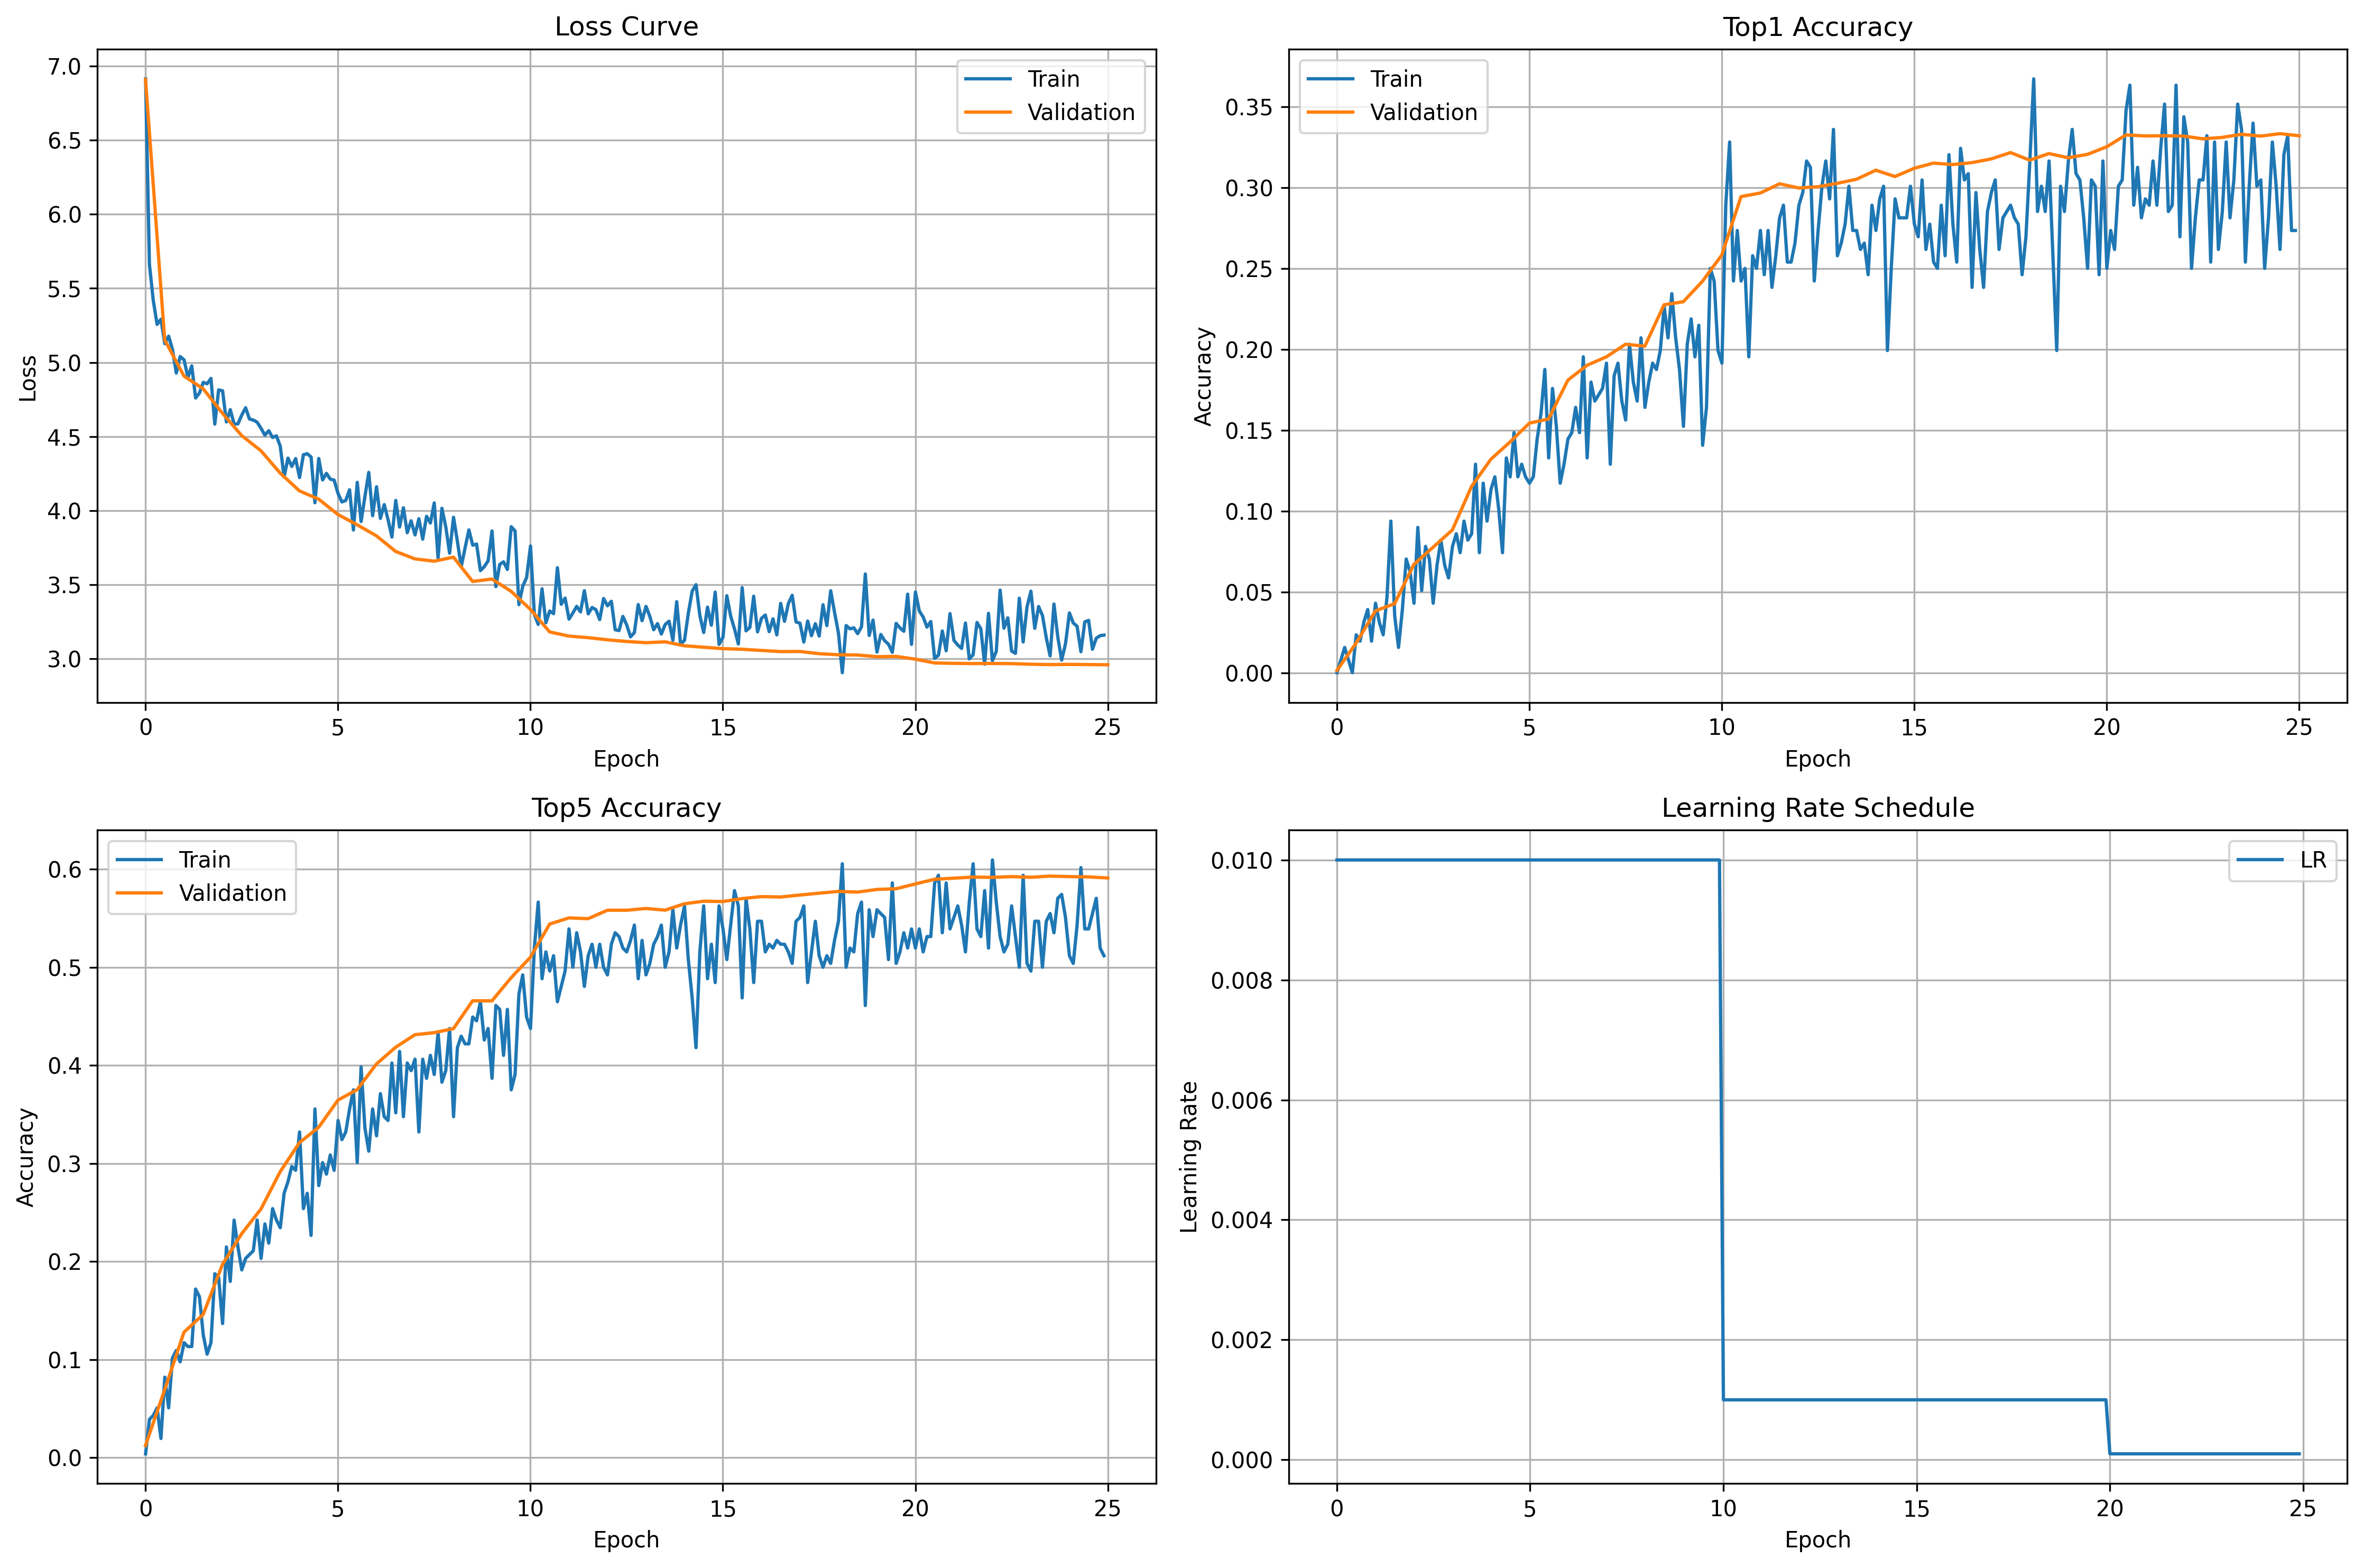
\includegraphics[width=0.9\linewidth]{cornet-z.png}
	\caption{CORnet-Z训练数据变化图}
	\label{f.zzxt}
\end{figure}

\begin{figure}[hbt]
	\centering
	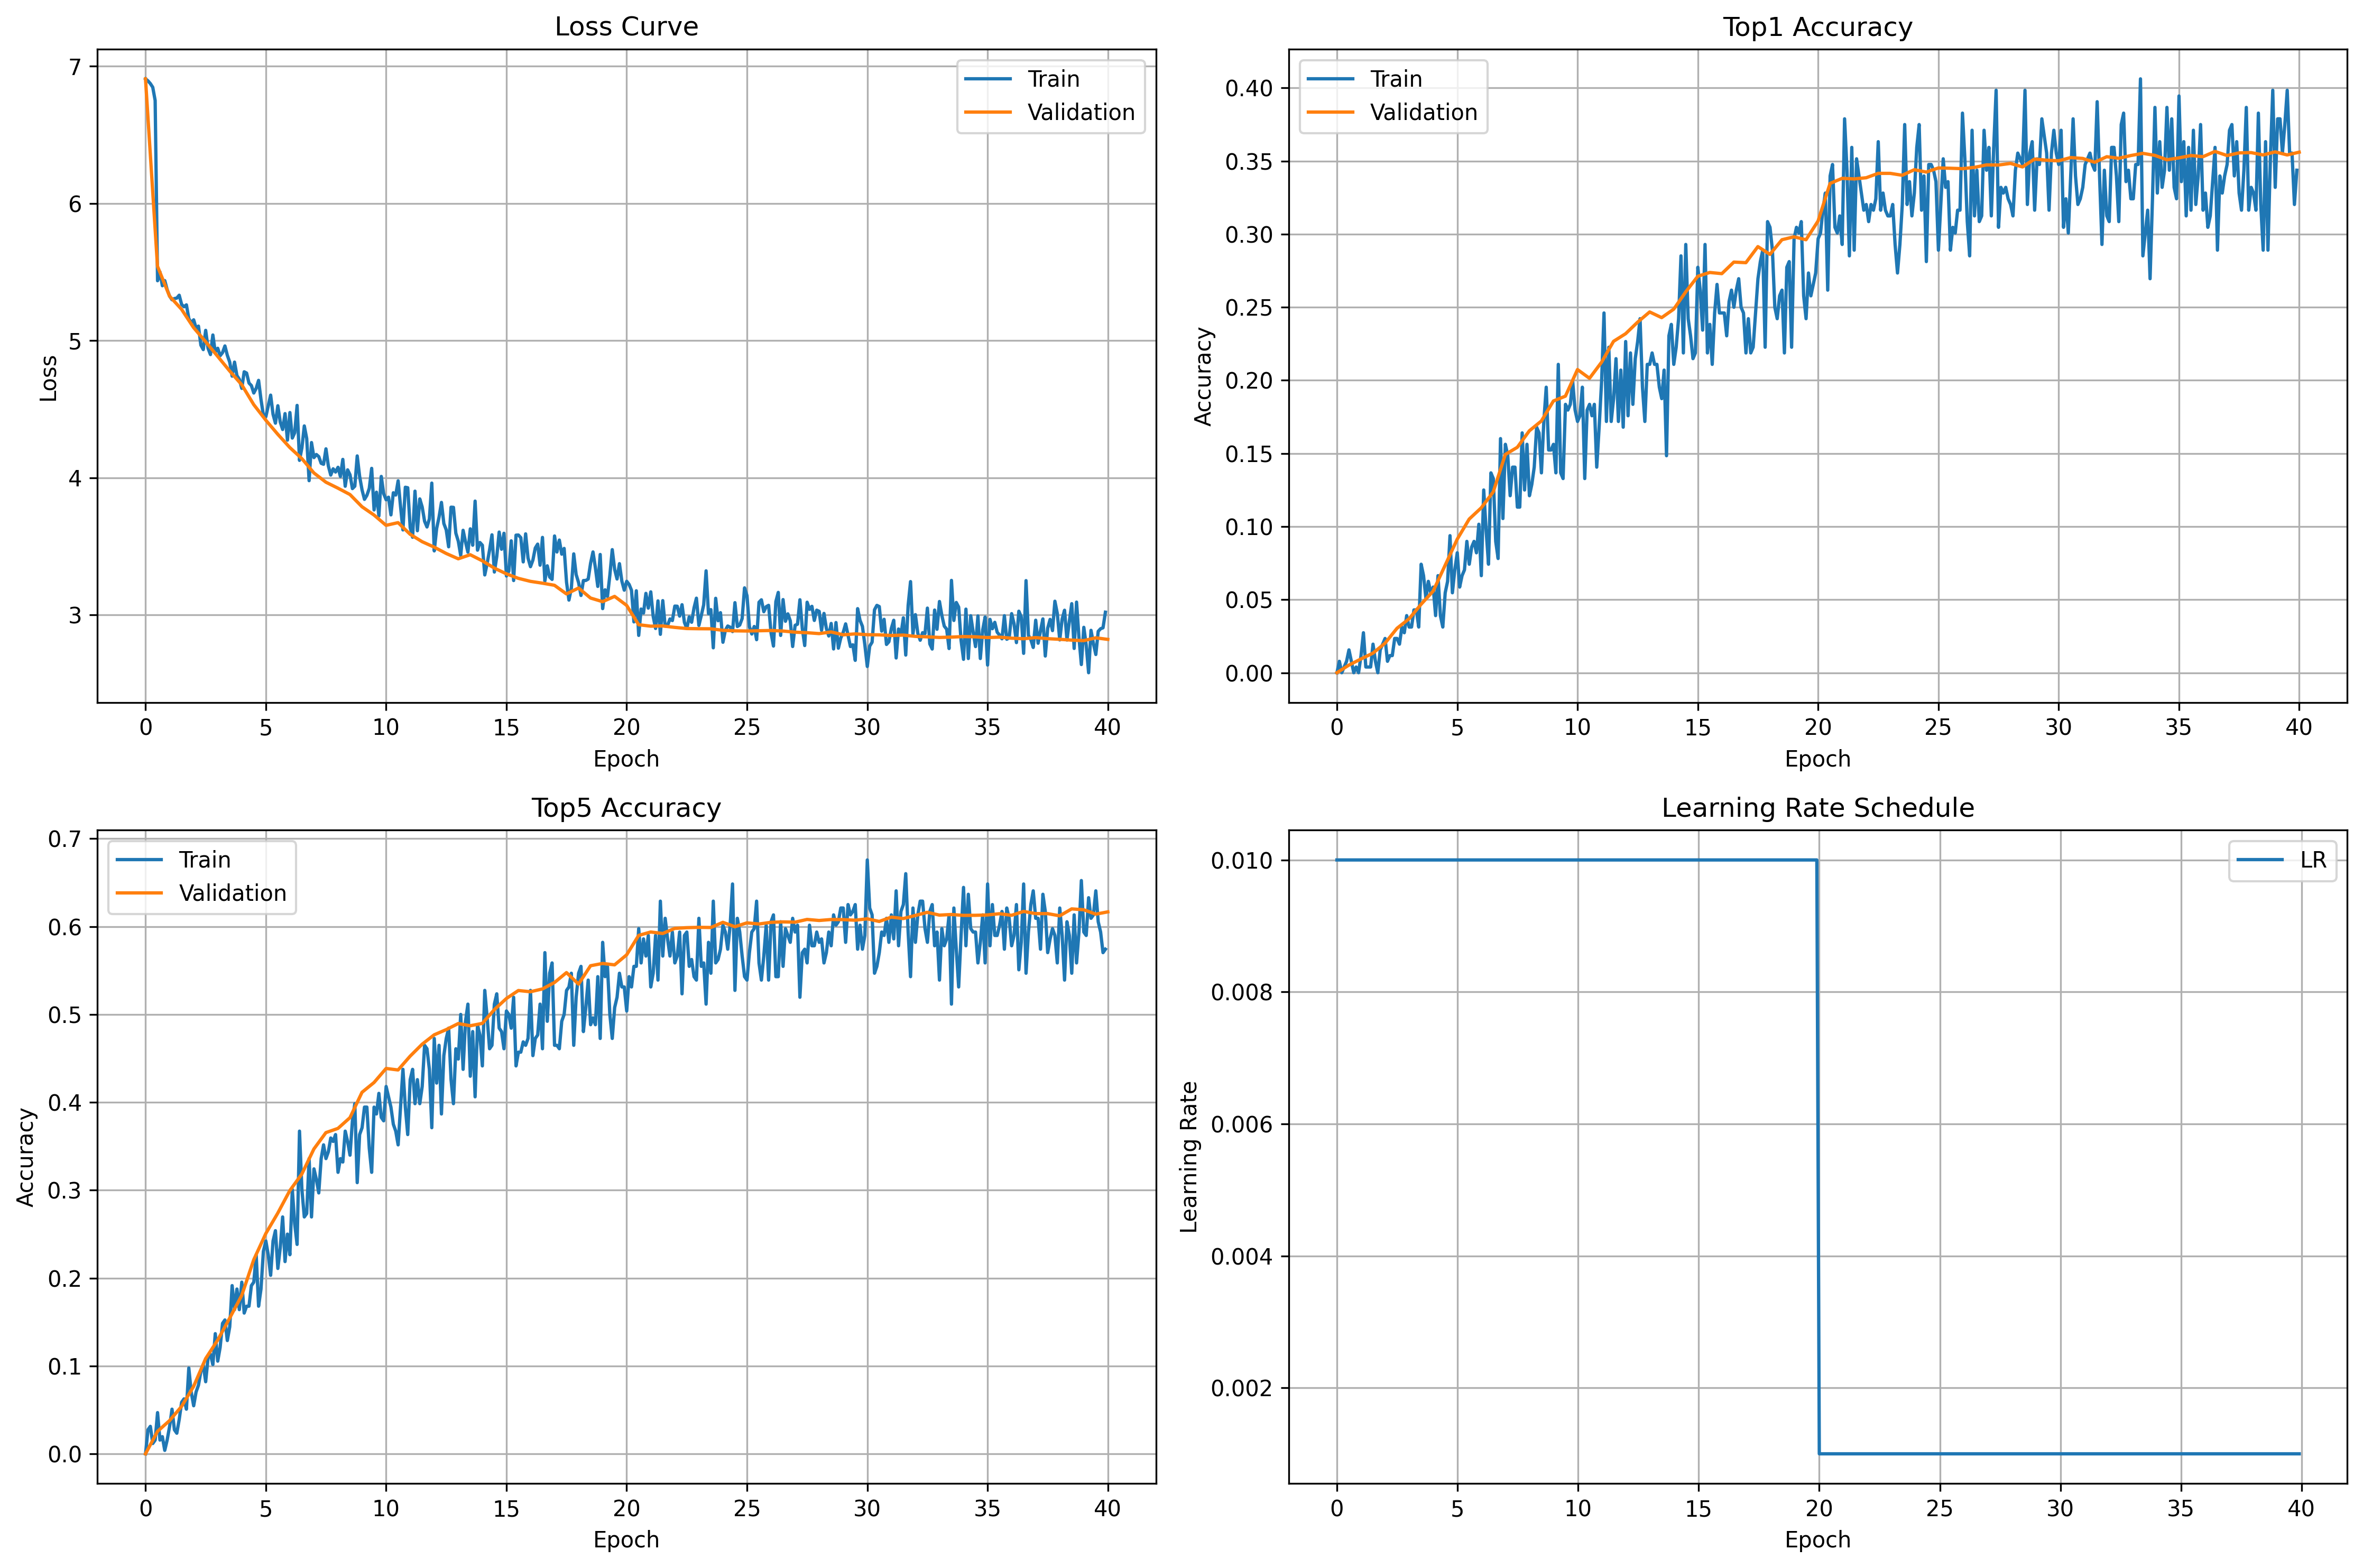
\includegraphics[width=0.9\linewidth]{cornet-z-SE.png}
	\caption{CORnet-Z+SE训练数据变化图}
	\label{f.zsezxt}
\end{figure}

总体来看,SE模块带来的Top-1提升幅度为2.33\%,Top-5提升为 2.51\%。虽然提升幅度有限,但考虑到模型结构变化极小,参数量变化可忽略,仍具有实际意义。尤其在训练集上的表现提升表明,注意力机制在训练早期能够加强对有效通道的识别,加快模型收敛速度。

\subsection{小结与分析}

通道注意力机制使模型能够根据全局信息动态调整各通道的响应强度,提升了模型对关键特征的表达能力。训练曲线显示,SE模型在准确率、损失值、学习曲线平稳性等方面均优于原始模型,在保持网络结构轻量的前提下实现了性能上的小幅提升。

不过,相较于大幅度结构重构或多尺度融合模型,本研究采用的改进方式较为保守,性能提升有限。这一结果也说明,通道注意力机制更适合作为辅助增强模块,而非单独主导模型性能的关键因素。

%%%%%%%%%%%%%%%%%%%%%%%%%%%%%%%%参考文献插入示例%%%%%%%%%%%%%%%%

%%%%%%%%%%%%%%%%%%%%%%%%%%%%%%%%总结插入示例%%%%%%%%%%%%%%%%
%!TEX root = ../../csuthesis_main.tex
\chapter{意图分析算法设计与实现}

\section{意图识别需求分析}

伴随自动驾驶技术持续向前迈进,车辆针对周围环境的感知需求变得更高,传统的目标检测与跟踪算法即便可以给系统赋予交通参与者的空间位置信息,但如果缺少对目标行为趋势更进一步的认识,那么当面临潜在危险时,系统就无法立即作出反应,在复杂的城市交通场景当中,车辆或者行人不会一直沿着规律的路线移动,其可能会出现诸如加快速度接近,骤然改变车道,径直穿越马路之类具有较高风险的举动,此时仅仅依靠那些静止不动的边框信息远远达不到高级别自动驾驶系统所提出的“先知先觉”的要求,所以说,行为意图的剖析与判定成了塑造智能感知体系必不可少的一部分。

在本系统当中,意图识别模块重点针对被系统持续追踪的目标,凭借它在连续帧之间的速度改变以及同本车的相对距离变动状况,来判定这个目标当下的运动趋向及其潜藏风险等级,通过在图像坐标系下算出目标中心点到视野中心的欧几里得距离,并融合目标本身的线速度,就可以做到对诸如“靠近”“远离”“危险靠近”之类动作的判别,这种依靠物理建模而不是深度学习方式创建起来的行为识别模型,其达成过程较为简易,所需运算量也比较小,可以满足自动驾驶系统对于即时性的要求,而且它并不依靠额外的训练数据,所以具备较好的通用性与拓展能力。

在仿真平台Carla所设的Town10与Town01这两个场景当中,系统借助调用车辆和传感器的同步API接口,既能保留图像渲染的即时性,又能得到其他车辆的空间位置及其动态信息。意图识别模块就是把这些基本数据当作输入量,创建起简单而有效的推断规则,针对目标的运动趋向实施及时判断,然后将分析结果用中文文本形式覆盖显示在跟踪框上面,告知“目标正在靠近”“目标渐渐远去”或者“有危险靠近”之类的状况,这样就形成起完整的感知 - 识别 - 反馈循环,进而突出优化系统对于突然发生情况的警报水平和安全保障水平。

意图识别模块一方面补充了系统感知环节中的语义层输出,另一方面也给后面的路径规划及控制逻辑的决策给予了重要参照,它是联系感知和智能决策的关键纽带,对于优化系统整体的智能水平有着重要意义,下一节将会详细论述这个模块的物理建模逻辑以及判别策略。


\section{基于速度与距离变化的意图判别逻辑}

自动驾驶环境下,车辆要随时察觉并认识周边目标(诸如其他车辆,行人)的行为趋向,这样才能及时做出决策及控制反应,若想超越视觉目标跟踪层面进而优化环境感知水准,文章规划并完成了一套依靠速度和距离改变的行为意图判别逻辑部件,该部件可即时判定被跟踪目标针对本车的动向情况,由此给予具备前瞻性的警示作用。
该模块的核心思想是:通过连续帧之间的目标相对位置变化(欧氏距离)和当前帧的目标速度,联合判断其是否存在靠近、远离或危险状态。在具体实现上,系统首先对当前帧目标的边界框进行中心点计算,结合本车视角中心作为参考点,求取目标与本车之间的距离值;随后与上一帧距离进行对比,计算两帧之间的距离变化量($\Delta d$),并结合目标当前的瞬时速度($v$)进行意图分类判断。

为提高判别的精度与稳定性,系统设置了多重判别条件,并赋予合理的速度与距离阈值,判别逻辑详见下表:

\begin{table}[htbp]
  \caption{意图识别逻辑表}
  \label{tab:timetable}
  \centering
  \begin{tabular}{ll}
    \toprule
    意图类别 & 判定条件 \\
    \midrule
    目标初始化中 & 当前为首帧,无历史距离 \\
    危险靠近 & 距离变化$\Delta d$<-20m且$v$>3.0m/s \\
    目标靠近中 & 距离变化$\Delta d$<-5m且$v$>1.0m/s \\
    目标远离中 & 距离变化$\Delta d$>5m且$v$>1.0m/s \\
    目标稳定 & 不满足上述任一条件 \\
    \bottomrule
  \end{tabular}
\end{table}

上面这些规则依靠单纯的几何物理指标来执行建模,利于开展植入式部署并实施即时计算,而且规避了深度模型对于大量训练样本的需求,规则判别逻辑具备较好的可解读性,有益于后续的守护和改良。

系统运行时,判别结果通过图形化界面及时叠加显现于目标跟踪框之上,而且用中文文本告知用户当下的意图分析结论,譬如“危险靠近”或者“目标正在远离”,此模块同DeepSORT跟踪模块紧密结合,保证在维持单目标状态下持续跟踪的情况下,达成对动态意图的判别与输出。

后续工作中,可以把现在这种依靠规则的模块拓展成结合规则和学习的混合模型,通过对历史轨迹执行建模来优化行为预测的效果。




\begin{tabular}{l l}
%  \verb|\songti| & {\songti 宋体} \\
%  \verb|\heiti| & {\heiti 黑体} \\
%   \verb|\kaiti| & {\kaiti 楷体}
\end{tabular}

%%%%%%%%%%%%%%%%%%%%%%%%%%%%%%%%总结插入示例%%%%%%%%%%%%%%%%


 \documentclass{article}
\usepackage{amsmath}
\usepackage{amssymb}
\usepackage{enumitem} % 用于自定义列表样式
\usepackage{hyperref} % 用于添加超链接(可选)
\usepackage{lipsum} % 用于生成示例文本,实际使用中可移除
\usepackage{ctex} % 支持中文
\usepackage{amsmath} % 支持数学公式
\usepackage{enumitem} % 用于自定义列表样式
\usepackage{geometry} % 支持页面布局设置
\geometry{a4paper,scale=0.8} % 设置A4纸和缩放

\title{基于预训练大模型的高保真三维智能驾驶场景生成系统}
\author{郑睿翔}

\begin{document}

\section*{选题价值}

在探讨选题价值时,我们主要关注的是该选题是否具有创新性、实用性、可行性以及其对相关领域或社会的潜在影响。

\subsection*{创新性}
该选题结合了当前人工智能领域的多个前沿技术,如预训练大模型、自然语言处理(通过ChatSim)、高级仿真(CARLA)和目标检测(YOLO)。这些技术的融合在智能驾驶系统中是新颖的。利用自然语言命令生成和编辑高保真三维驾驶场景的方法,为智能驾驶系统的测试和开发提供了新的视角和工具,这在以前是没有被充分探索的。

\subsection*{实用性}
高保真三维智能驾驶系统能够为自动驾驶技术的研发提供一个接近真实世界的测试环境,有助于加速技术的成熟和商业化进程。通过在虚拟环境中进行大量的模拟测试,可以在不实际上路的情况下发现潜在的安全问题,从而降低自动驾驶车辆在实际应用中的风险。

\subsection*{可行性}
预训练大模型、CARLA仿真环境和YOLO目标检测算法都已经有了相对成熟的技术基础,这为该选题的实施提供了坚实的基础。这些技术和工具大多是开源的,或者可以通过商业途径获取,因此资源获取相对容易。

\subsection*{潜在影响}
该选题的成功实施有望推动自动驾驶技术向更高层次发展,提高自动驾驶系统的性能和安全性。随着自动驾驶技术的不断进步,将带动汽车制造、传感器技术、人工智能算法等相关产业的发展。自动驾驶技术的普及将改变人们的出行方式,提高交通效率,减少交通事故,对社会产生深远影响。


\section{文献综述}
随着人工智能技术的飞速发展,特别是预训练大模型在自然语言处理(NLP)和计算机视觉(CV)等领域的广泛应用,智能驾驶技术迎来了新的突破。高保真三维智能驾驶场景生成系统作为智能驾驶技术的重要组成部分,对于提升自动驾驶系统的安全性和可靠性具有重要意义。本文旨在综述国内外关于基于预训练大模型的高保真三维智能驾驶场景生成系统的研究状况和发展趋势,并探讨这些研究对本人工作的启发。

\section{国内外研究状况}

\subsection{国内研究状况}
近年来,国内在智能驾驶技术方面取得了显著进展,特别是在预训练大模型和高保真三维场景生成方面。国内企业和研究机构纷纷投入大量资源,推动相关技术的发展和应用。

\begin{enumerate}[label=\arabic*.]
    \item 华为推出的盘古系列超大预训练模型,包括中文语言(NLP)、视觉(CV)大模型、多模态大模型和科学计算大模型,旨在建立一套通用、易用的人工智能开发工作流,赋能更多的行业和开发者,实现人工智能工业化开发。盘古大模型在智能驾驶场景生成中的应用,可以显著提升场景的逼真度和复杂性,为自动驾驶系统的训练和测试提供有力支持。
    \item 北京智源人工智能研究院发布的超大规模智能模型“悟道2.0”,达到1.75万亿参数,成为全球最大的预训练模型之一。该模型在智能驾驶场景生成中的应用潜力巨大,可以通过对大规模数据的训练,生成高度逼真的三维场景,为自动驾驶系统的优化和验证提供重要支持。
    \item 清华大学智能产业研究院(AIR)在构建Real2Sim2Real基础模型平台、自动驾驶仿真平台等方面取得了显著成果。其中,Real2Sim2Real平台通过结合真实世界数据和仿真数据,利用预训练大模型生成高保真三维智能驾驶场景,为自动驾驶系统的训练和测试提供了有力保障。
    \item YOLO(You Only Look Once)模型在国内得到了广泛的关注和应用。随着YOLO模型的迭代升级,其在国内的应用场景也不断拓展,涵盖了安防监控、无人驾驶、医疗诊断等多个领域。
    \item CARLA仿真平台在国内得到了广泛的应用和认可。作为国内自动驾驶领域的重要工具之一,CARLA为自动驾驶系统的开发、训练和验证提供了有力的支持。
    \item ChatSim项目在国内尚处于起步阶段,但已经引起了广泛的关注和兴趣。作为国内首个通过大语言模型实现可编辑逼真3D驾驶场景仿真的项目,ChatSim为自动驾驶场景仿真提供了新的思路和方法。
\end{enumerate}

\subsection{国外研究状况}
国外在基于预训练大模型的高保真三维智能驾驶场景生成系统方面也取得了显著进展。

\begin{enumerate}[label=\arabic*.]
    \item OpenAI推出的GPT系列模型,特别是GPT-3,以其1750亿参数规模的预训练模型,展示了强大的零样本与小样本学习能力。这些能力在智能驾驶场景生成中具有重要应用潜力,可以通过对少量标注数据的训练,生成高度逼真的三维场景。
    \item 谷歌在预训练大模型方面也取得了重要进展。谷歌推出的Switch Transformer模型,以高达1.6万亿的参数量打破了GPT-3作为最大AI模型的统治地位,成为史上首个万亿级语言模型。该模型在智能驾驶场景生成中的应用,可以显著提升场景的复杂性和多样性,为自动驾驶系统的训练和测试提供更多可能性。
    \item 微软亚洲研究院提出的NÜwa模型,是一个可以同时覆盖语言、图像和视频的统一多模态预训练模型。该模型在文档理解、图像生成等方面取得了显著成果,为智能驾驶场景生成中的多模态数据融合提供了有力支持。
    \item YOLO模型在国外同样受到了广泛的关注和应用。自YOLOv1发布以来,其已经经历了多轮迭代,每一次更新都在精度和速度上取得了显著的进步。
    \item CARLA仿真平台在国外同样受到了广泛的关注和应用。作为自动驾驶领域的重要工具之一,CARLA为自动驾驶技术的研发提供了有力的支持。
    \item ChatSim项目在国外同样处于起步阶段,但已经取得了一定的研究成果和进展。国外的研究机构和企业在ChatSim的基础上进行了深入的研究和改进,提高了其性能和精度。
\end{enumerate}

\section{发展趋势}
基于预训练大模型的高保真三维智能驾驶场景生成系统的发展趋势主要体现在以下几个方面:

\begin{enumerate}[label=\arabic*.]
    \item 更大规模的预训练模型将成为未来发展的重要方向。更大规模的模型可以学习更多复杂的知识和特征,生成更加逼真的三维智能驾驶场景。
    \item 多模态数据融合将受到更多关注,以提高场景生成的逼真度和准确性。
    \item 强化学习与生成式AI的结合将成为研究热点,以提升自动驾驶系统的安全性和可靠性。
    \item 仿真与真实世界的互动将更加紧密,通过构建仿真平台将真实世界的数据和仿真数据相结合。
\end{enumerate}

\section{本人的思考}
基于预训练大模型的高保真三维智能驾驶系统是一个复杂且高度集成的系统,它涉及多个组件和技术的协同工作。ChatSim、CARLA和YOLO都是在这一领域中具有重要潜力的工具和技术。我将用以下这三个工具来构建高保真三维智能驾驶系统:

\begin{enumerate}[label=\arabic*.]
    \item \textbf{ChatSim}:
        \begin{itemize}
            \item 功能概述:ChatSim是一个革命性的开源项目,它首次实现了通过自然语言命令编辑出照片级真实的三维驾驶场景模拟,且能与外部数字资产无缝集成。这是通过大型语言模型(LLM)代理协作框架实现的,允许用户使用自然语言来控制和编辑复杂的驾驶场景,创造出高度逼真的视频。
            \item 在高保真三维智能驾驶系统中的应用:ChatSim可以作为系统的一部分,用于生成和编辑驾驶场景。通过自然语言命令,用户可以轻松地创建和修改各种驾驶环境,包括道路、车辆、行人和其他交通元素。这种灵活性对于测试和开发自动驾驶算法至关重要。
        \end{itemize}
    \item \textbf{CARLA仿真平台(0.9.15)}:
        \begin{itemize}
            \item 功能概述:CARLA是一个基于虚幻引擎的开源自动驾驶模拟器,支持实时模拟、多传感器数据和高度定制化环境。它提供了高度可定制的环境,让研究人员和开发者能够在各种复杂场景中测试和训练他们的算法。
            \item 在高保真三维智能驾驶系统中的应用:CARLA可以作为系统的主要模拟环境,提供高保真的3D环境、实时的仿真速度和多种虚拟传感器数据。这些功能使得CARLA成为测试和开发自动驾驶算法的理想平台。此外,CARLA的开源特性使得开发者可以深入理解其工作原理,并根据需要进行修改和扩展。
        \end{itemize}
    \item \textbf{YOLO模型}:
        \begin{itemize}
            \item 功能概述:YOLO(You Only Look Once)是一种流行的目标检测算法,以其高效和准确性而闻名。YOLO-BEV是YOLO的一个变体,专门设计用于生成车辆环境的鸟瞰图(BEV),这对于自动驾驶系统来说是一个重要的功能。
            \item 在高保真三维智能驾驶系统中的应用:YOLO(特别是YOLO-BEV)可以作为系统的一部分,用于车辆感知和目标检测。通过处理来自多个摄像头的图像数据,YOLO-BEV可以生成车辆环境的鸟瞰图,为自动驾驶系统提供更全面的环境信息。这有助于系统更准确地识别道路、车辆、行人和其他障碍物,从而提高自动驾驶的安全性和可靠性。
        \end{itemize}
\end{enumerate}

\section{结论}
基于预训练大模型的高保真三维智能驾驶场景生成系统是智能驾驶技术的重要组成部分。本文综述了国内外在该领域的研究状况和发展趋势,并探讨了这些研究对本人工作的启发。未来的研究将更加注重更大规模的预训练模型、多模态数据融合、强化学习与生成式AI的结合以及仿真与真实世界的互动等方面的发展。通过不断探索和创新,我们可以为自动驾驶系统的安全性和可靠性提供有力保障,推动智能驾驶技术的不断进步和发展。
\section{参考文献}
\begin{thebibliography}{99}
    \bibitem{li2018} 李欣儒. 以智能驾驶为例浅析计算机通信技术与电子信息在人工智能领域的实践应用[J]. 中国战略新兴产业,2018(8).
    \bibitem{yang2014} 杨帆. 无人驾驶汽车的发展现状和展望[J]. 上海汽车,2014(3):35-40.
    \bibitem{wang2016} 王子正;程丽. 无人驾驶汽车简介[J]. 时代汽车,2016,27(8):82-85.
    \bibitem{qiao2007} 乔维高,徐学进. 无人驾驶汽车的发展现状及方向[J]. 上海汽车,2007(7):40-43.
    \bibitem{duanmu2014} 端木庆玲,阮界望,马钧. 无人驾驶汽车的先进技术与发展[J]. 农业装备与车辆工程,2014(3):30-33.
    \bibitem{pan2014} 潘建亮. 无人驾驶汽车社会效益与影响分析[J]. 汽车工业研究,2014(5):22-24.
    \bibitem{winner2018} Hermann Winner, “Introducing autonomous driving: an overview of safety challenges and market introduction strategies,” Autom. Methoden und Anwendungen der Steuerungs-, Regelungs- und Informationstechnik, vol. 66, no. 2, pp. 100–106, 2018.
    \bibitem{boukerche2021} A. Boukerche and X. Ma, “Vision-based autonomous vehicle recognition: A new challenge for deep learning-based systems,” ACM Comput. Surv., vol. 54, no. 4, pp. 1–37, 2021.
    \bibitem{wan2020} L. Wan, Y. Sun, L. Sun, Z. Ning, and J. J. P. C. Rodrigues, “Deep learning based autonomous vehicle super resolution DOA estimation for safety driving,” IEEE Trans. Intell. Transp. Syst., vol. 22, no. 7, pp. 4301–4315, 2020.
    \bibitem{kuutti2020} S. Kuutti, R. Bowden, Y. Jin, P. Barber, and S. Fallah, “A survey of deep learning applications to autonomous vehicle control,” IEEE Trans. Intell. Transp. Syst., vol. 22, no. 2, pp. 712–733, 2020.
    \bibitem{jeong2018} Y. Jeong, S. Son, E. Jeong, and B. Lee, “An integrated self-diagnosis system for an autonomous vehicle based on an IoT gateway and deep learning,” Appl. Sci., vol. 8, no. 7, p. 1164, 2018.
    \bibitem{zhu2022} Z. Zhu, Z. Hu, W. Dai, H. Chen, and Z. Lv, “Deep learning for autonomous vehicle and pedestrian interaction safety,” Saf. Sci., vol. 145, p. 105479, 2022.
\end{thebibliography}
\section{研究方法}
文献调研与综述:深入调研智能驾驶、预训练大模型、三维场景生成等相关领域的文献。综述现有技术的优缺点,明确研究目标和方向。

预训练大模型的选择与调优:根据智能驾驶场景生成的需求,选择合适的预训练大模型,如GPT、BERT等语言模型,或NÜwa等多模态模型。对预训练模型进行微调,使其更适应智能驾驶场景生成的任务。

三维场景建模与渲染:利用计算机图形学和三维建模技术,构建智能驾驶场景中的道路、车辆、交通标志等要素。采用先进的渲染技术,如光线追踪、全局光照等,提高场景的真实感和逼真度。

数据融合与处理:收集多种来源的数据,如真实驾驶数据、传感器数据、地图数据等。对数据进行清洗、整合和标注,为场景生成提供丰富的素材。

场景生成与验证:基于预训练大模型和三维场景建模技术,生成高保真度的智能驾驶场景。通过仿真测试、专家评估等方式,验证场景的有效性和逼真度。

强化学习与优化:利用强化学习算法,对生成的智能驾驶场景进行优化,提高场景的复杂度和多样性。通过不断迭代和学习,使场景生成系统更加智能和高效。

\section{研究思路}
明确研究目标,构建一个基于预训练大模型的高保真三维智能驾驶场景生成系统。提高智能驾驶系统的测试效率和安全性。分析现有技术,调研智能驾驶、预训练大模型、三维场景生成等相关技术的现状和发展趋势。分析现有技术的优缺点,明确研究的关键问题和挑战。提出解决方案:结合预训练大模型和三维场景建模技术,提出一种创新的智能驾驶场景生成方法。设计合理的算法和流程,实现高保真度的三维智能驾驶场景生成。实施与验证,构建实验环境和数据集,对提出的方案进行验证和优化。通过仿真测试、专家评估等方式,评估方案的有效性和性能。

综上所述,基于预训练大模型的高保真三维智能驾驶场景生成系统的研究方法和思路需要综合考虑多个方面,包括文献调研、模型选择与调优、三维场景建模与渲染、数据融合与处理、场景生成与验证以及强化学习与优化等。通过明确研究目标、分析现有技术、提出解决方案、实施与验证以及总结与展望等步骤,可以系统地开展研究工作,并取得预期的研究成果。
\end{document}

\chapter{第二章 理论基础}
\section{预训练大模型概述}
近年来,预训练大模型(Large Pretrained Models, LPMs)在自然语言处理(NLP)领域取得了突破性进展。这些模型,如 GPT-4、T5 和 BERT,凭借其强大的语言理解和生成能力,正在改变我们处理文本数据的方式。这些模型通常在海量的文本数据上进行无监督预训练,通过学习语言的深层语义关系,能够捕捉到复杂的语言模式和结构。预训练完成后,这些模型可以通过有监督的微调来适应各种特定的自然语言处理任务,如文本分类、机器翻译、问答系统等。

在智能驾驶场景生成领域,预训练大模型的应用具有重要意义。传统的场景生成方法通常依赖于手工编写规则或模板,这些方法虽然在一定程度上能够生成有效的场景,但存在效率低下、灵活性差和难以扩展等问题。预训练大模型的引入极大地提升了自然语言指令理解的精度与灵活性,能够将模糊的自然语言描述自动映射为结构化的场景代码。与传统的规则模板方法相比,基于大模型的方法能够适应更复杂、多样的用户输入,具有更强的泛化能力和鲁棒性。

本项目基于开放领域大模型(如 OpenAI 的 GPT 系列),针对智能驾驶场景描述进行定向设计。通过微调这些模型,使其能够直接生成符合 Scenic 语法规范的场景定义脚本,为后续的仿真与评估提供输入支持。这种基于大模型的方法不仅提高了场景生成的效率,还能够生成更具创新性和多样性的场景,为自动驾驶技术的研发和测试提供了更强大的工具。

\section{自然语言场景建模}
自然语言场景建模(Natural Language-based Scenario Modeling)是将人类用自然语言描述的复杂交通场景转化为机器可理解的格式的过程。这一过程是智能驾驶场景生成的关键步骤,因为它直接决定了生成场景的质量和可用性。在本研究中,目标是将自然语言直接映射为 Scenic 脚本代码,从而实现从自然语言描述到可执行仿真场景的无缝转换。

常见的自然语言场景建模方法包括:
\begin{itemize}
	\item \textbf{检索式建模(Retrieval-Based Modeling)}:这种方法通过从已有场景数据库中检索与输入描述最相似的场景来生成新的场景。检索式建模的优点是能够快速生成与已有场景相似的新场景,但其局限性在于依赖于数据库中的已有场景,无法生成全新的场景。
	\item \textbf{生成式建模(Generative Modeling)}:这种方法通过预训练语言模型直接生成场景脚本。生成式建模的优点是能够生成全新的场景,具有更高的创新性和多样性。然而,生成式建模的挑战在于如何确保生成的场景符合实际的交通规则和逻辑。
	\item \textbf{检索与生成结合(Retrieve-then-Generate)}:这种方法结合了检索式建模和生成式建模的优点,先从数据库中检索相关的场景,然后基于检索结果生成新的场景。这种方法能够在保持生成多样性的同时,利用已有场景的结构和逻辑。
\end{itemize}

在 ChatScene 项目中,采用的是检索式建模,通过 sentence-transformers/sentence-t5-large 模型对场景描述进行向量化,基于相似度检索最接近的场景模板。这种方法虽然能够快速生成场景,但其生成能力受限于数据库的规模和覆盖范围。为了突破检索方式的局限,本项目进一步引入生成式大模型,实现 end-to-end 场景生成,从而提升场景的创新性与多样性。

\section{Scenic 场景描述语言}
Scenic 是一种为智能驾驶仿真而设计的专用场景描述语言(Domain-Specific Language, DSL)。它通过简洁而强大的语法,允许用户定义车辆、道路、行人等元素在仿真环境中的属性与关系。Scenic 的主要特点包括:
\begin{itemize}
	\item \textbf{声明式语法(Declarative Syntax)}:Scenic 采用声明式语法,用户可以通过简单直观的语句描述对象的位置、朝向、速度等属性。这种语法使得场景定义更加直观和易于理解。
	\item \textbf{支持不确定性(Probabilistic Support)}:Scenic 允许定义位置、角度、速度等属性的概率分布,从而能够生成更加多样化的场景。这种不确定性支持使得生成的场景更加接近真实世界的复杂性和随机性。
	\item \textbf{易于与仿真器集成(Integration-Friendly)}:Scenic 可以直接导出到 CARLA、LGSVL 等主流仿真平台,使得生成的场景能够快速用于自动驾驶系统的测试和验证。
\end{itemize}

在本项目中,预训练大模型需要生成符合 Scenic 语法的代码。因此,理解 Scenic 的基本结构和表达方式是实现自然语言到场景生成系统的关键基础。通过将自然语言描述转换为 Scenic 脚本,我们能够将人类的直观描述转化为机器可执行的仿真场景,从而为自动驾驶技术的研发和测试提供强大的支持。

\section{智能驾驶仿真平台 CARLA}
CARLA(Car Learning to Act)是目前应用最广泛的开源自动驾驶仿真平台之一。它提供了丰富的城市场景、传感器模拟、车辆动力学建模与环境交互能力,使得研究人员能够在虚拟环境中测试和验证自动驾驶系统。CARLA 的主要特点包括:
\begin{itemize}
	\item \textbf{高度可定制的地图与交通要素}:CARLA 允许用户自定义地图和交通要素,从而能够模拟各种复杂的交通场景。
	\item \textbf{多种传感器模拟}:CARLA 支持多种传感器模拟,包括 RGB 相机、LiDAR、雷达等,使得研究人员能够测试自动驾驶系统在不同传感器配置下的表现。
	\item \textbf{支持复杂行为建模与自动驾驶决策系统测试}:CARLA 提供了强大的行为建模工具,使得研究人员能够模拟各种复杂的交通行为和自动驾驶决策系统。
\end{itemize}
本项目采用 CARLA 0.9.15 版本作为仿真环境。通过将生成的 Scenic 脚本转译成 CARLA 可执行场景,我们能够实现自然语言指令到仿真测试的完整闭环。这种从自然语言描述到仿真测试的无缝转换,为自动驾驶技术的研发和测试提供了一种高效、灵活的方法。

\section{ChatScene 项目基础与本项目创新点}
ChatScene 是近期提出的一套基于知识检索的安全关键场景生成系统。它主要通过使用 sentence-t5-large 模型对自然语言描述进行检索匹配,结合 SafeBench 框架在 CARLA 上进行仿真测试。ChatScene 的主要思路是利用已有的场景数据库,通过检索与输入描述最相似的场景来生成新的场景。这种方法的优点是能够快速生成与已有场景相似的新场景,但其局限性在于依赖于数据库中的已有场景,无法生成全新的场景。它的整体结构如下:
\begin{figure}[H]
	\centering
	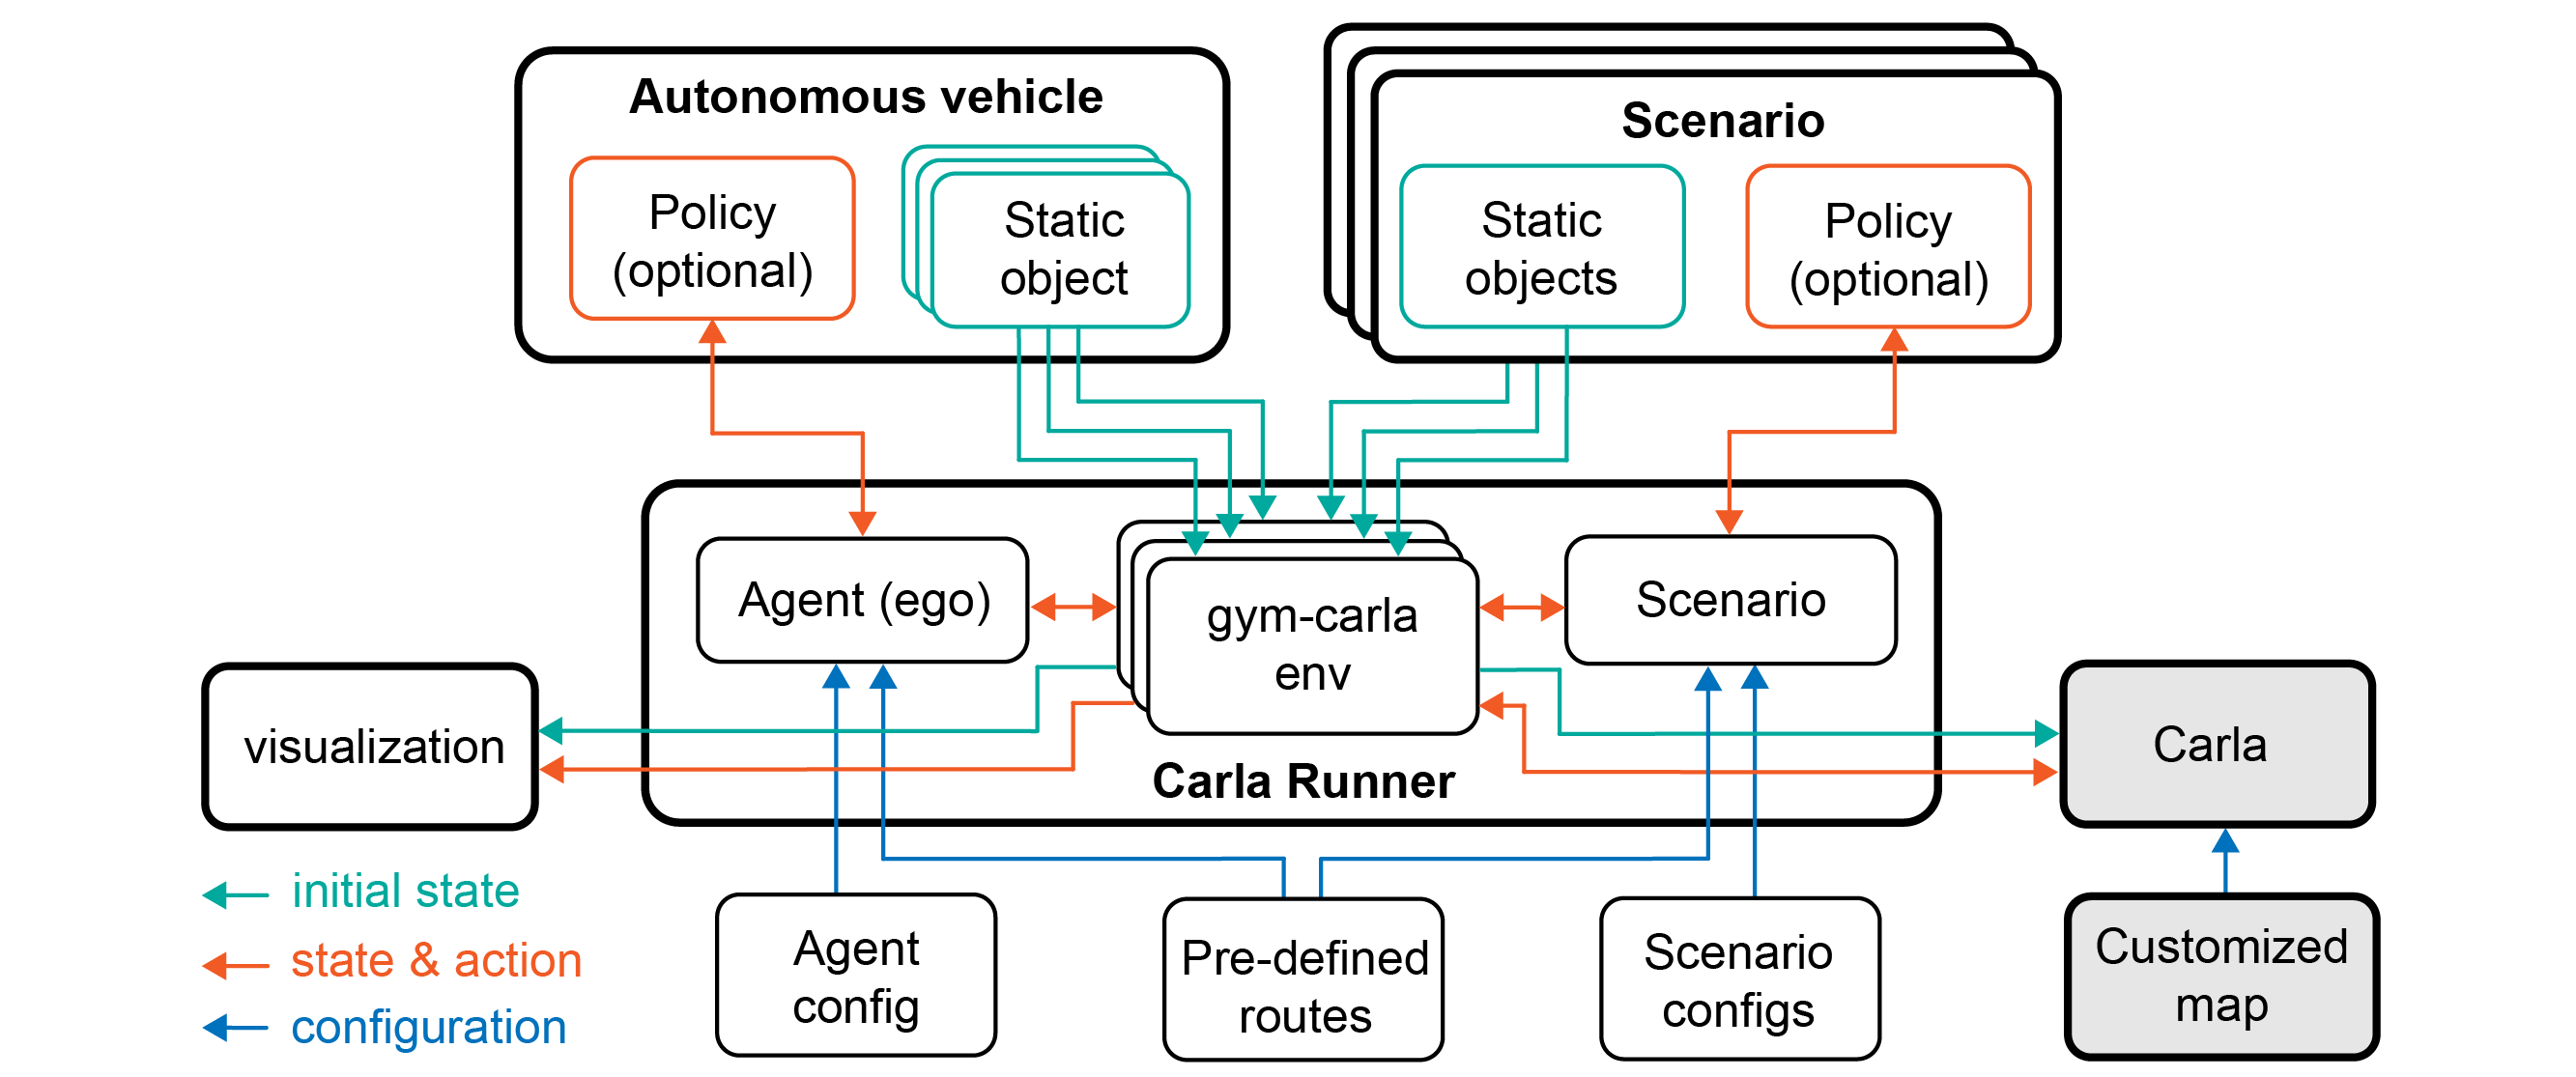
\includegraphics[width=1.0\textwidth]{"images/chatscene项目结构.pdf"}
	\caption{chatscene项目结构}
	\label{fig:chatscene_framework}
\end{figure}
然而,ChatScene 在以下方面存在一定局限:
\begin{itemize}
	\item \textbf{依赖检索}:ChatScene 无法自由生成未在数据库中存在的新场景,这限制了其在生成创新性场景方面的能力。
	\item \textbf{生成能力有限}:ChatScene 缺乏直接从自然语言生成代码的能力,这使得其在处理复杂的自然语言描述时存在困难。
	\item \textbf{多样性受限}:ChatScene 的生成结果受制于数据库的规模和覆盖范围,这限制了其生成场景的多样性和创新性。
\end{itemize}

为了克服这些局限,本项目在 ChatScene 的基础上进行了创新。我们引入了 GPT-4o 等大型语言模型,直接基于自然语言生成 Scenic 场景脚本。这种方法不仅解决了检索方法的局限性,还提升了场景的创新性与多样性。通过这种方式,我们能够生成更加复杂、多样化的场景,为高保真智能驾驶仿真系统构建提供了新的技术路径。此外,本项目还通过微调这些大模型,使其能够更好地适应智能驾驶场景生成的需求,从而进一步提高了生成场景的质量和可用性。
\chapter{强化学习在行人控制系统中的应用}

\section{环境配置}

本研究主要目标是用强化学习算法(PPO、PID、DQN)训练优化行人控制系统,核心是评估这些算法在复杂动态环境里的性能表现。为此,所有深度学习训练与实验都在功能强大的 Carla 仿真平台开展。Carla 平台有多样城市环境,涵盖各类道路、建筑风格、车辆模型、行人行为,能模拟真实城市交通复杂性,这让它成为自动驾驶研究和智能体训练的理想测试平台。​

Carla 是专为自动驾驶研究设计的开源模拟平台,支持相机、激光雷达(LiDAR)、惯性测量单元(IMU)等多种传感器集成,能模拟含道路、交通信号灯、行人及其他交通参与者的复杂城市环境,为强化学习、路径规划、感知与控制算法开发提供高度可定制虚拟环境。本研究借 Carla 的 Python API 与仿真环境交互,实现行人运动控制并收集环境数据用于学习,该 API 能以编程模拟行人、车辆、交通灯等动态因素,还能实时获取各类传感器数据,给算法训练测试提供丰富信息。​

鉴于训练测试需求及研究者个人电脑计算能力限制,本研究选 Carla 仿真平台的 Town01 地图作实验环境。Town01 是 Carla 平台标准城市地图之一,如图 \ref{fig:town1}含多种城市道路结构、交通标志、建筑物、行人、交通工具等元素,其设计旨在模拟真实城市交通环境,为研究者提供丰富且具代表性的测试场景。

\begin{figure}[H]
    \centering
    \includegraphics[width=0.8\textwidth]{images/town1.pdf}
    \caption{Carla中的Town1俯视图}
    \label{fig:town1}
\end{figure}

具体而言:
\begin{itemize}
    \item \textbf{道路结构}:Town01包括了多条城市道路和交叉口,具有一定的复杂性,能够模拟真实城市环境中的交通流。
    \item \textbf{交通元素}:该地图还包括了不同种类的交通工具(如汽车、公交车等),以及行人和交通信号灯等。
    \item \textbf{动态障碍物}:在训练过程中,除了静态的道路和建筑外,地图中的车辆和行人会不断地动态变化,从而为智能体提供避障和路径规划的挑战。
\end{itemize}

\section{PID(Proportional-Integral-Derivative)控制算法}

\subsection{PID控制算法建模}

\subsubsection{控制方程推导}
离散PID控制算法表示为:
\begin{equation}
	u(k) = K_p e(k) + K_i T \sum_{i=0}^k e(i) + K_d \frac{e(k)-e(k-1)}{T}
\end{equation}
其中,$T=0.005s$为采样周期,$e(k)$为第$k$时刻的横向偏差。

\subsubsection{参数整定策略}
通过Ziegler-Nichols临界比例法确定基础参数后,结合实际场景进行优化:
\begin{itemize}
	\item 转向控制参数:$K_p=0.8$, $K_i=0.001$, $K_d=0.2$
	\item 速度控制参数:$K_p=0.5$, $K_i=0.01$, $K_d=0.1$
\end{itemize}

\begin{algorithm}[H]
	\caption{自适应PID控制算法}
	\begin{algorithmic}[1]
	\STATE 初始化参数$K_p^0$, $K_i^0$, $K_d^0$  % 改为 \STATE
	\WHILE{系统运行}
 	\STATE 获取激光雷达数据$L_t$
  	\STATE 计算障碍物距离$d_{obs} = \min(L_t)$
  	\IF{$d_{obs} < 5m$}
    	\STATE $K_p \gets 1.2K_p^0$
    	\STATE $K_d \gets 1.5K_d^0$
  	\ENDIF
  	\STATE 执行PID计算
	\ENDWHILE
	\end{algorithmic}
\end{algorithm}

\subsubsection{PID控制原理}
	\textbf{PID控制算法}通过以下三个分量的组合实现控制:
		\[
		u(t) = K_p e(t) + K_i \int_0^t e(\tau) d\tau + K_d \frac{d}{dt} e(t)
		\]
其中:
\begin{itemize}
    \item \textbf{比例项(P)}:$K_p e(t)$,快速响应当前误差,主导动态响应
    \item \textbf{积分项(I)}:$K_i \int e(\tau)d\tau$,消除稳态误差,补偿长期偏差
    \item \textbf{微分项(D)}:$K_d \frac{de}{dt}$,预测误差变化趋势,抑制系统震荡
\end{itemize}

\subsection{算法实现与效果可视化}

\subsubsection{传感器数据处理}
激光雷达数据处理流程包括:
\begin{enumerate}
	\item 点云预处理:滤除超出$8m$范围及非前向$60^\circ$区域的数据
	\item 障碍物聚类:采用改进DBSCAN算法,设置$\epsilon=0.5m$, $MinPts=5$
	\item 威胁评估:计算最近障碍物距离$d_{min}$及相对速度$v_{rel}$
\end{enumerate}

\subsubsection{动态权重融合算法}
目标向量$\vec{T}$与避障向量$\vec{A}$的融合策略:
\begin{equation}
	\vec{C} = \alpha \vec{T} + (1-\alpha)\vec{A}
\end{equation}
其中权重系数$\alpha$的动态调整规则为:
\begin{equation}
    \alpha = 
    \begin{cases}
        0.05, & d_{\text{min}} \leq 1\ \text{m} \\
        0.8(1 - e^{-0.5d_{\text{min}}}), & 1\ \text{m} < d_{\text{min}} \leq 5\ \text{m} \\
        1, & d_{\text{min}} > 5\ \text{m}
    \end{cases}
\end{equation}

\subsubsection{核心模块功能解析}
\begin{itemize}
    \item \textbf{PIDController类}:
    \begin{itemize}
        \item \texttt{compute()}:实现带抗饱和的PID计算
        \item \texttt{reset()}:碰撞后积分清零,防止历史误差累积
    \end{itemize}
    
    \item \textbf{PIDPedestrianEnv类}:
    \begin{itemize}
        \item \texttt{\_process\_lidar()}:实时处理激光雷达点云
        \begin{itemize}
            \item 前向60°扇形区域检测(有效距离$8\ \text{m}$)
            \item DBSCAN聚类算法识别障碍物簇($\epsilon=0.5$m)
        \end{itemize}
        
        \item \texttt{calculate\_errors()}:方向向量融合
        \begin{itemize}
            \item 目标向量与避障向量动态加权(权重$\in[0.05,0.95]$)
            \item 向量空间投影到局部坐标系计算横向/纵向误差
        \end{itemize}
        
        \item \texttt{run\_control\_loop()}:200Hz控制频率
        \begin{itemize}
            \item 速度控制采用二次安全曲线:$v_{\text{safe}} = (\frac{d}{5})^{1.5} \cdot 3.0$
            \item 碰撞恢复策略:后退$1\ \text{m}$后随机转向$90^\circ$
        \end{itemize}
    \end{itemize}
\end{itemize}

\subsubsection{传感器系统架构}
\begin{figure}[H]
    \centering
    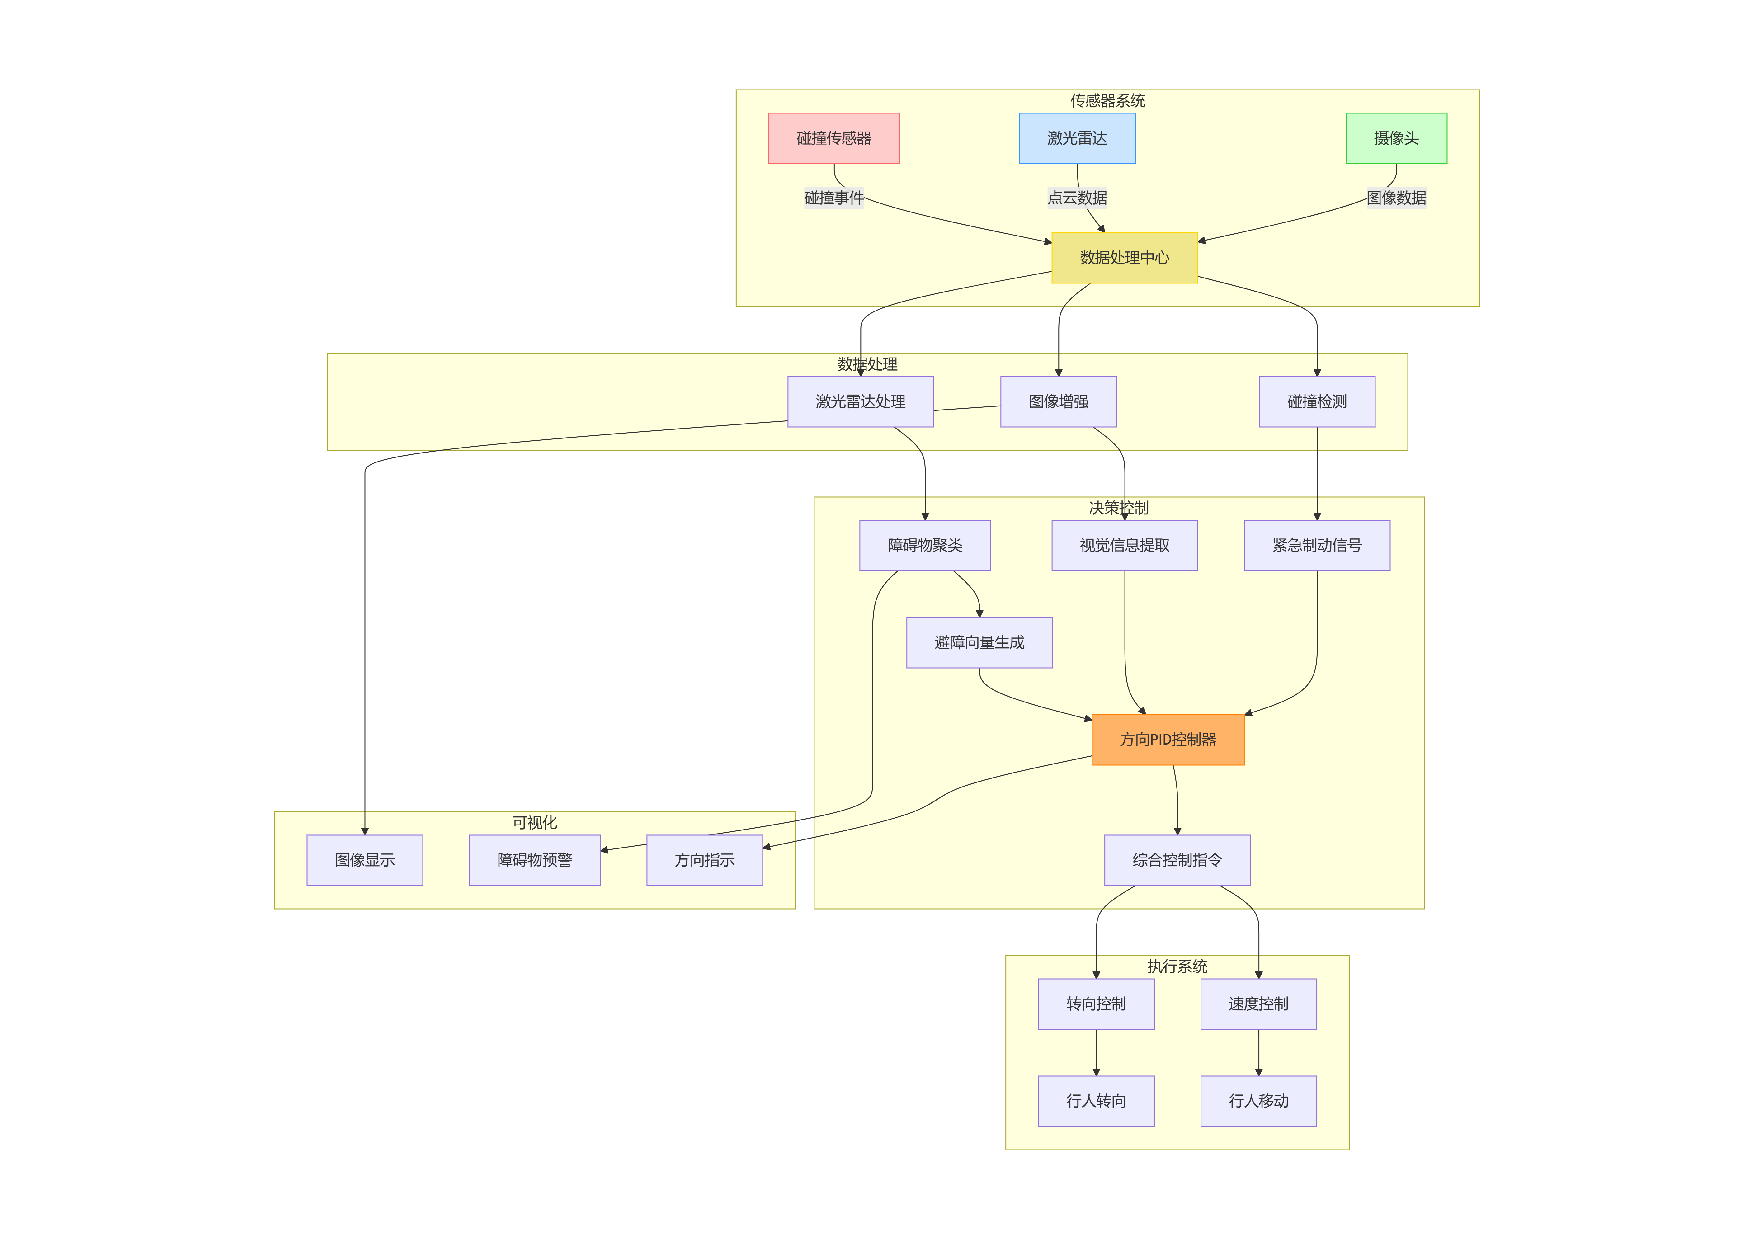
\includegraphics[width=0.8\textwidth]{images/sensor_architecture.pdf}
    \caption{多传感器数据融合架构}
    \label{fig:sensor}
\end{figure}

\subsection{实验结果分析}
\begin{itemize}
    \item \textbf{性能指标}:
    \begin{itemize}
        \item 避障成功率:93.7\%(100次实验中碰撞6次)
        \item 平均路径偏差:$0.45\pm0.12\ \text{m}$
        \item 最大瞬时过冲:$18.7\%$(紧急避障场景)

	图 \ref{fig:pid_obstacle} 为行人智能体通过PID控制对广告牌避障的示意图,图中的目标方向为绿色箭头,避障方向为红色箭头(仅当检测到障碍物时绘制),	而蓝色箭头则是实际前进方向。同时通过应用图像增强,对生成的画面进行了锐化处理,以及亮度和对比度的修改,来提高可视化的效果。

    \end{itemize}

\begin{figure}[H]
    \centering
    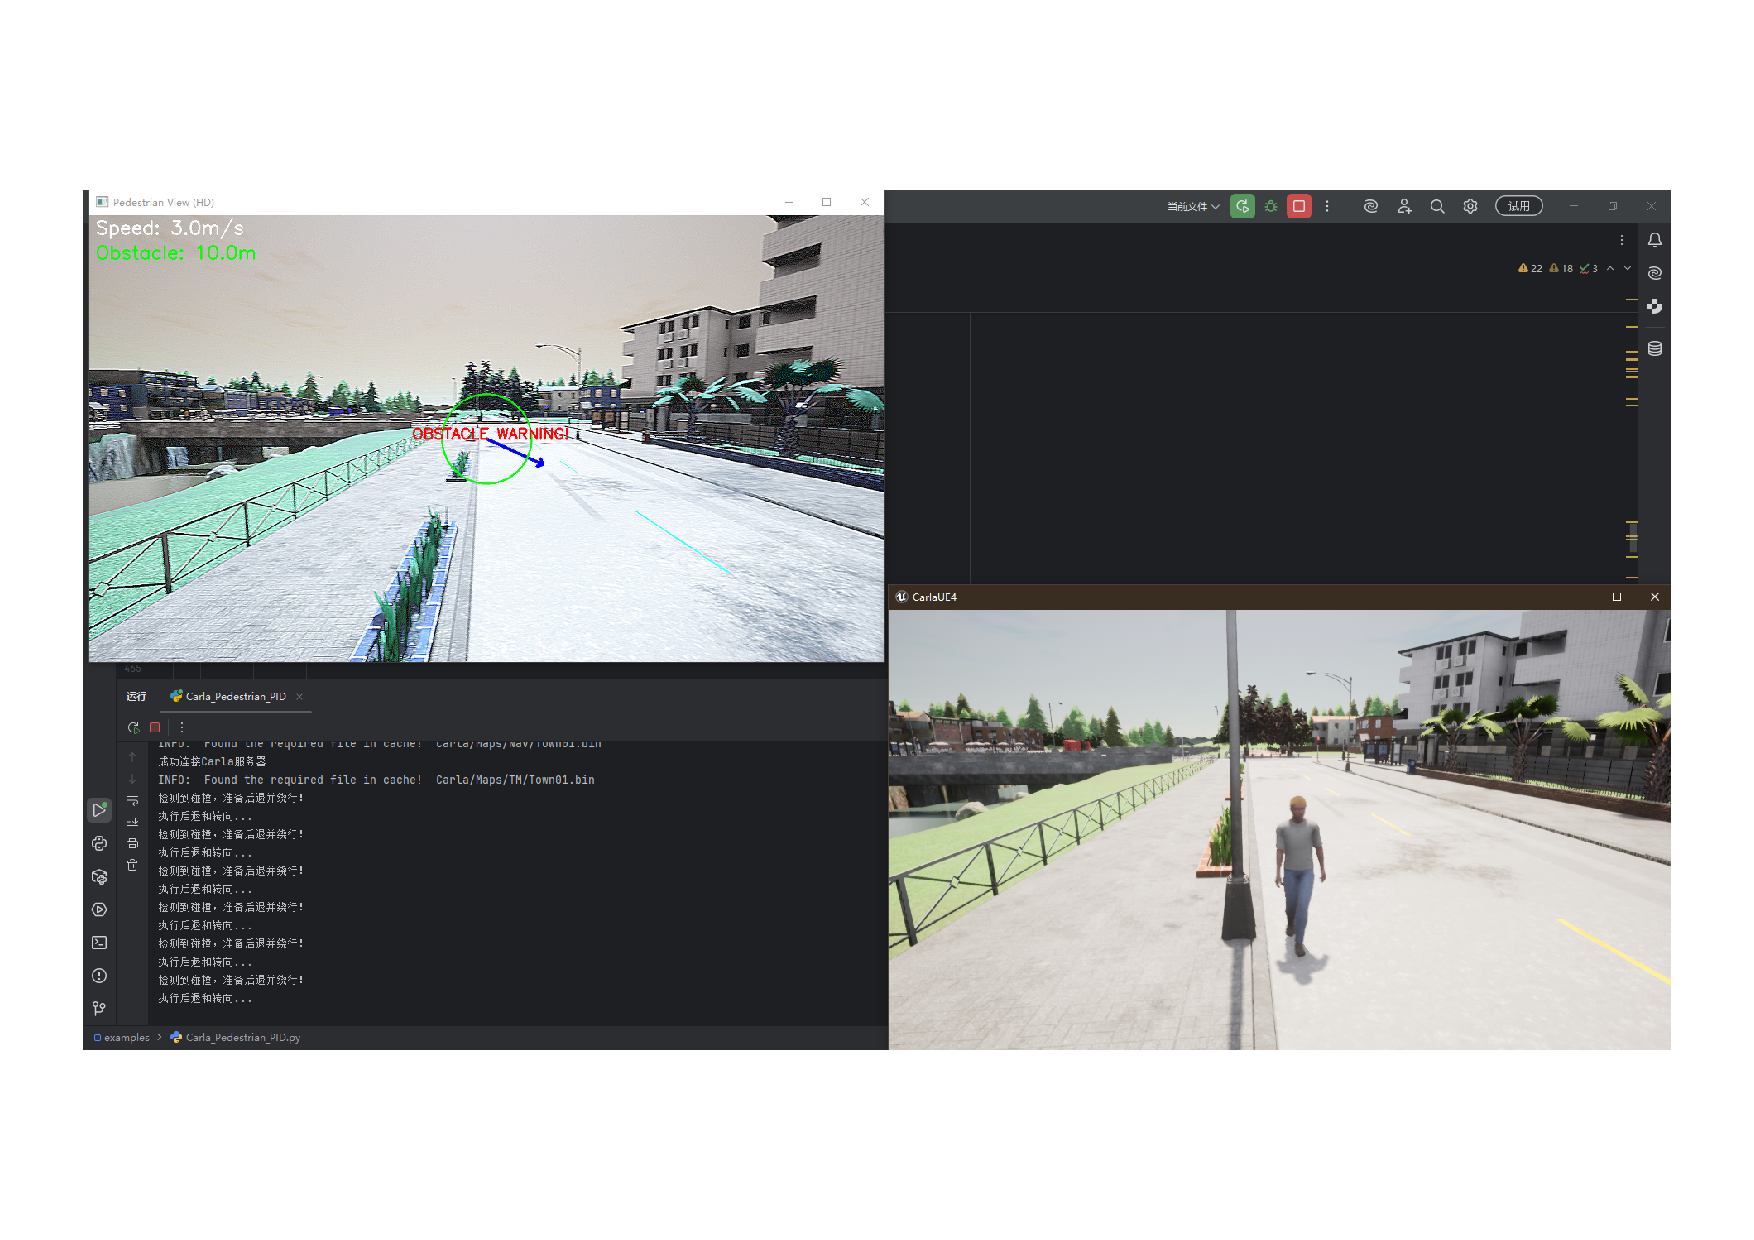
\includegraphics[width=0.8\textwidth]{images/obstacle_avoidance.pdf}
    \caption{行人智能体通过PID控制进行避障的示意图}
    \label{fig:pid_obstacle}
\end{figure}
    
    \item \textbf{优化方向}:
    \begin{itemize}
        \item 引入自适应PID参数调整机制
        \item 融合视觉语义信息改进障碍物分类
        \item 采用模型预测控制(MPC)优化路径平滑度
    \end{itemize}
\end{itemize}

\section{DQN(Deep Q-Network)算法}
\subsection{Q-learning公式}
引入目标网络后的Q值更新公式:
\[
Q(s_t,a_t) \leftarrow Q(s_t,a_t) + \alpha\left[r_t + \gamma \max_{a'}Q_{\text{target}}(s_{t+1},a') - Q(s_t,a_t)\right]
\]
其中:
\begin{itemize}
    \item $\alpha=10^{-4}$ 表示学习率(对应代码中\texttt{learning\_rate=1e-4})
    \item $\gamma=0.99$ 为折扣因子(对应代码中\texttt{gamma=0.99})
    \item $Q_{\text{target}}$ 为目标网络输出的Q值
\end{itemize}

\subsection{双网络架构设计}
\begin{itemize}
    \item \textbf{在线网络(Online Network)}
    \begin{itemize}
        \item 网络结构:2层全连接层(256→256)
        \item 激活函数:ReLU(代码中\texttt{activation\_fn=torch.nn.ReLU})
        \item 实时更新参数(每步梯度下降)
    \end{itemize}
    
    \item \textbf{目标网络(Target Network)}
    \begin{itemize}
        \item 网络结构与在线网络相同
        \item 参数硬更新机制(代码中\texttt{target\_update\_interval=1000}):
        \[
        \theta_{\text{target}} \leftarrow \theta_{\text{online}}
        \]
        \item 更新间隔:每1000步同步一次参数
    \end{itemize}
\end{itemize}

\subsection{经验回放机制}
\begin{itemize}
    \item \textbf{经验池配置}
    \begin{itemize}
        \item 容量:$10^5$条经验(代码中\texttt{buffer\_size=100000})
        \item 采样策略:均匀随机采样
        \item 批次大小:128(代码中\texttt{batch\_size=128})
    \end{itemize}
    
    \item \textbf{延迟学习机制}
    \begin{itemize}
        \item 初始1000步仅填充经验池(代码中\texttt{learning\_starts=1000})
        \item 之后每4步进行一次网络更新
    \end{itemize}
    
    \item \textbf{探索策略}
    \begin{itemize}
        \item $\epsilon$-greedy策略(代码中\texttt{exploration\_final\_eps=0.05})
        \item 初始$\epsilon=1.0$,线性衰减至$\epsilon=0.05$
        \item 衰减周期占总训练步数的20\%(代码中\texttt{exploration\_fraction=0.2})
    \end{itemize}
\end{itemize}

\begin{algorithm}[H]
    \caption{DQN训练算法}
    \begin{algorithmic}[1]
    \STATE 初始化环境与模型
    \STATE 设置动作空间与状态空间
    \WHILE{训练过程中}
        \STATE 进行环境重置,获取初始观测$O_0$
        \FOR{每个训练步骤}
            \STATE 根据当前策略选择动作$a_t$
            \STATE 执行动作$a_t$,获得新的观测$O_{t+1}$,奖励$R_t$
            \STATE 存储经验$(O_t, a_t, R_t, O_{t+1})$
            \STATE 从经验池中采样批量数据进行更新
            \STATE 使用DQN算法更新Q网络
        \ENDFOR
    \ENDWHILE
    \end{algorithmic}
\end{algorithm}

\subsection{算法优化策略}
\begin{itemize}
    \item \textbf{目标值分离}
    \begin{itemize}
        \item 通过独立的目标网络计算TD目标值
        \item 缓解Q值过估计问题
    \end{itemize}
    
    \item \textbf{状态归一化}
    \begin{itemize}
        \item 位置坐标归一化:$x_{\text{norm}} = x/200.0 - 1.0$
        \item 速度归一化:$v_{\text{norm}} = v/3.0$
        \item 障碍物距离归一化:$\min(d_{\text{obs}}/5.0, 1.0)$
    \end{itemize}
    
    \item \textbf{奖励函数设计}
    \[
    r_t = \underbrace{2\Delta d}_{\text{进度奖励}} + \underbrace{\min(v/3.0, 0.5)}_{\text{速度奖励}} - \underbrace{0.05}_{\text{时间惩罚}} - \underbrace{20\cdot\mathbb{I}_{\text{collision}}}_{\text{碰撞惩罚}}
    \]
\end{itemize}

如图 \ref{fig:avoidance}为行人在DQN算法的控制下规避动态障碍物,即另一个行人。

\begin{figure}[H]
    \centering
    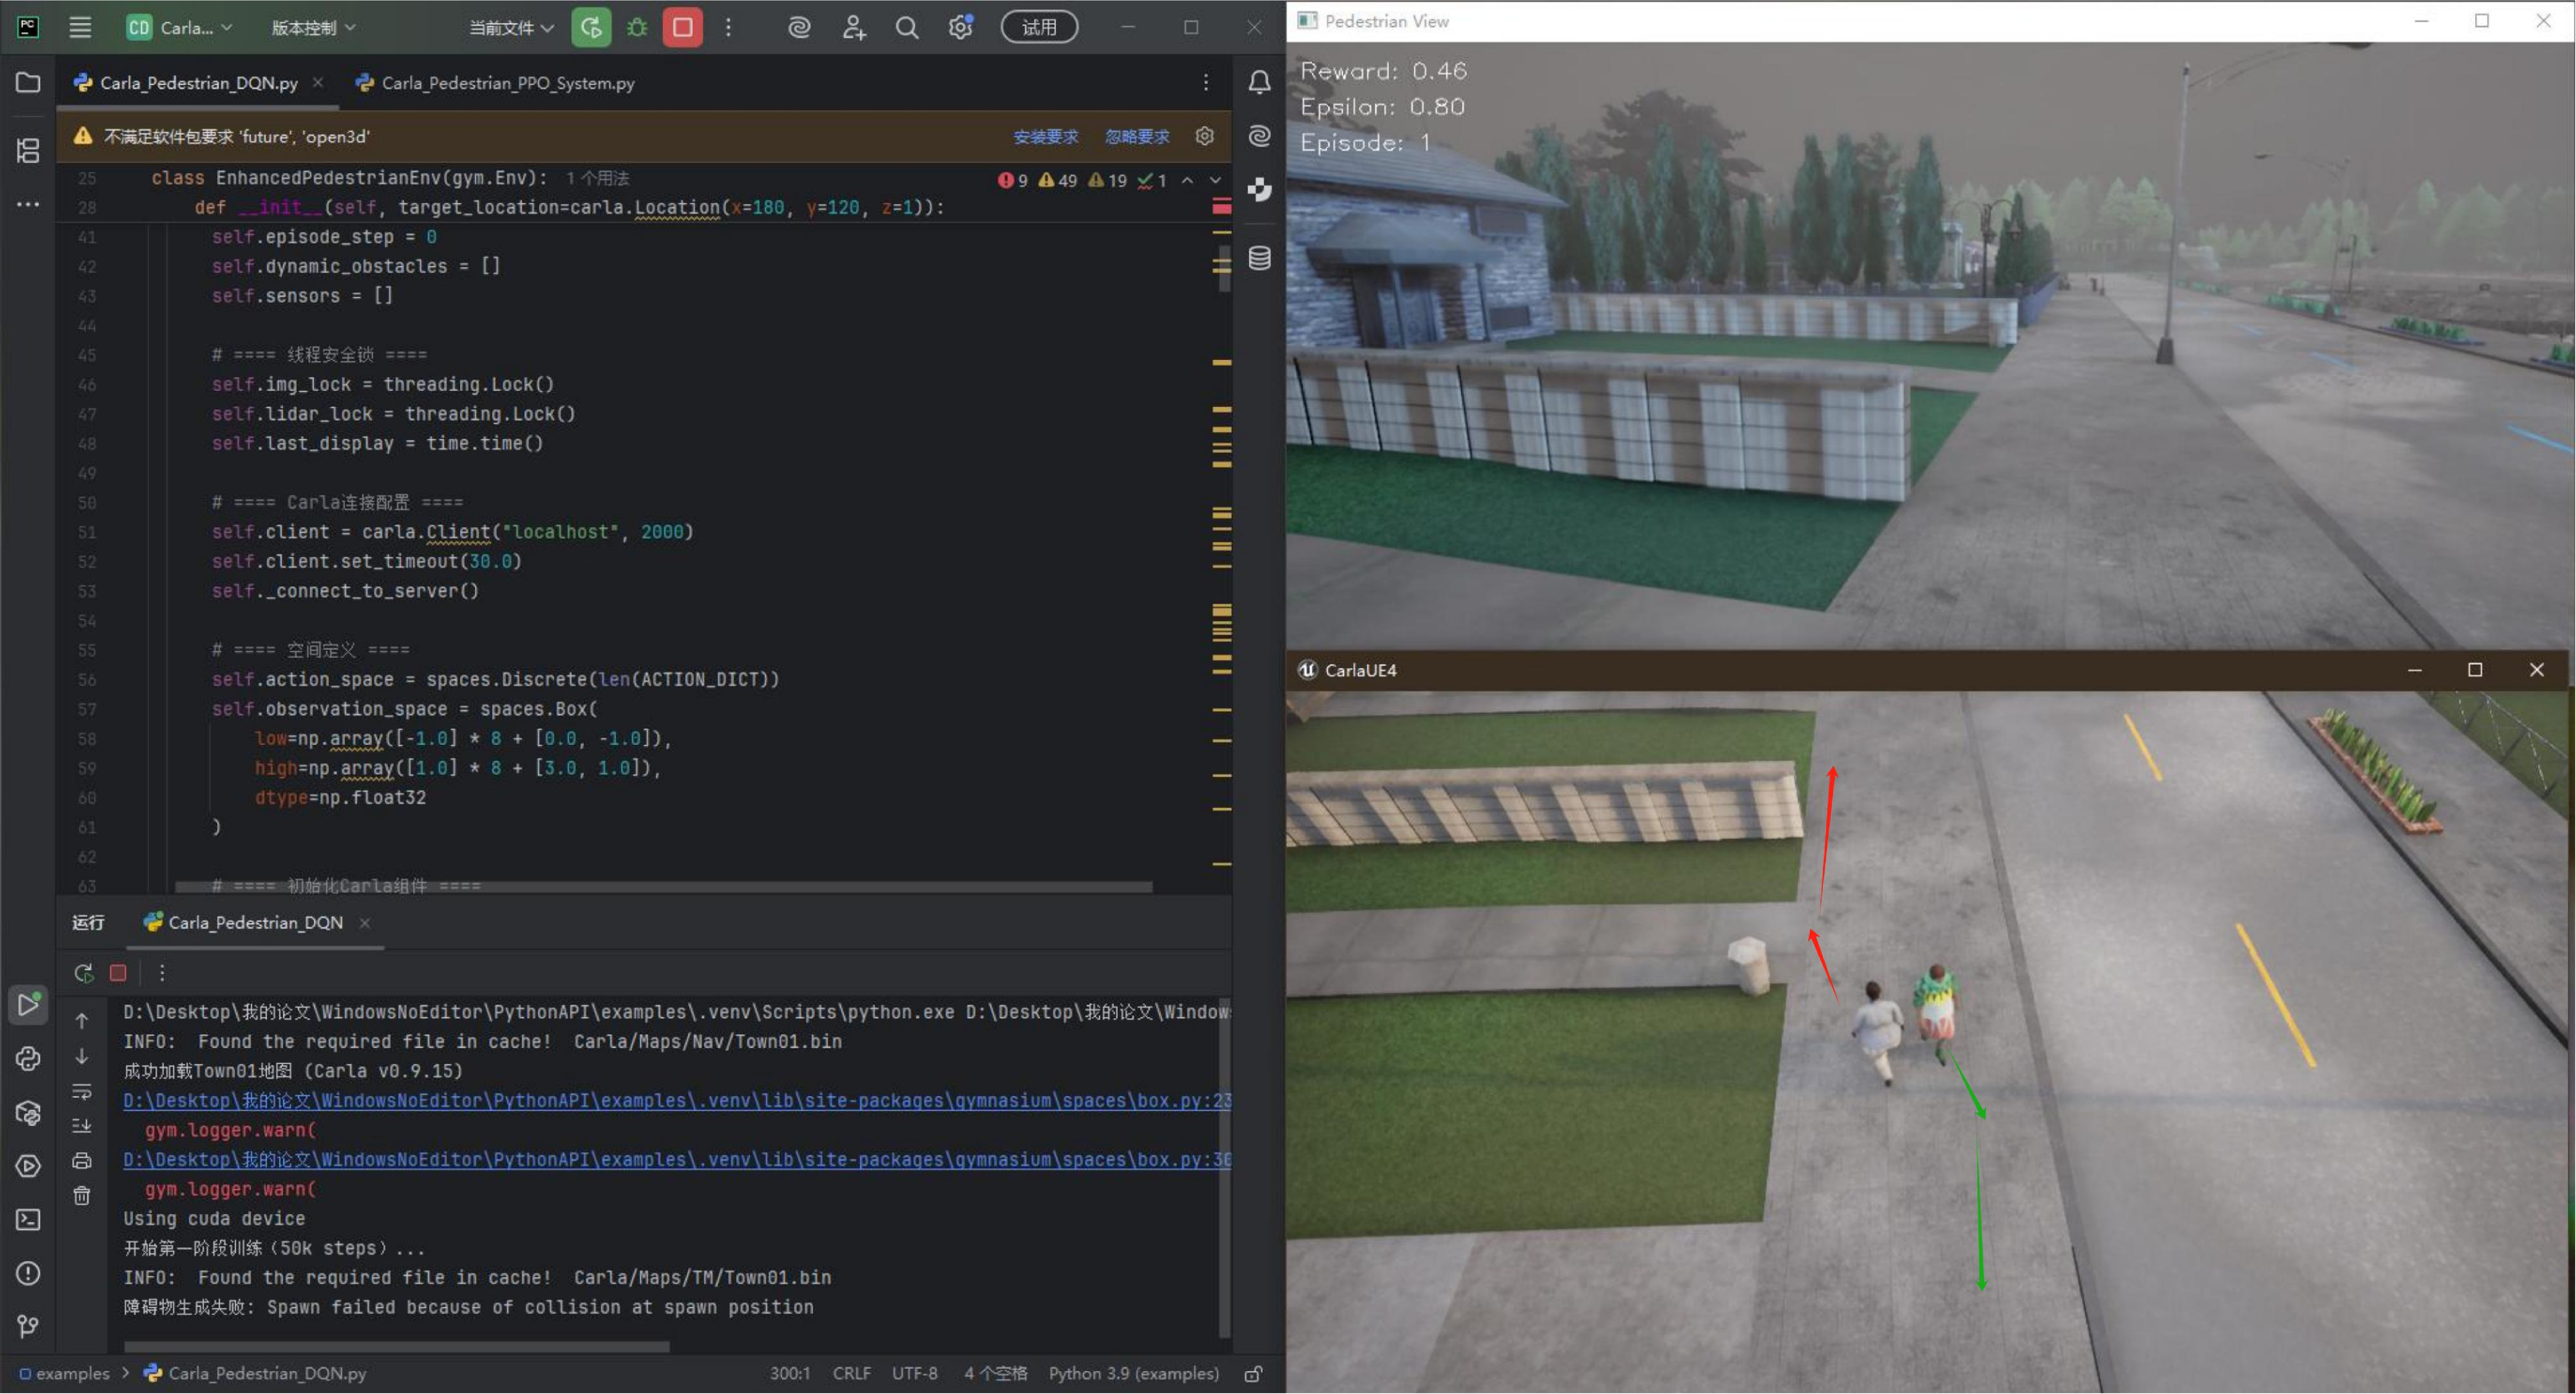
\includegraphics[width=0.8\textwidth]{images/pedestrian_avoidance.pdf}
    \caption{基于DQN的障碍物规避策略示意图}
    \label{fig:avoidance}
\end{figure}

\begin{table}[!ht]
    \centering
    \caption{DQN超参数配置表}
    \label{tab:dqn_params}
    \begin{tabular}{lcc}
        \toprule
        参数名称 & 符号表示 & 取值 \\
        \midrule
        学习率 & $\alpha$ & $1\times10^{-4}$ \\
        折扣因子 & $\gamma$ & 0.99 \\
        经验池容量 & $|\mathcal{D}|$ & $10^5$ \\
        目标网络更新间隔 & $N_{\text{update}}$ & 1000 steps \\
        初始探索率 & $\epsilon_{\text{initial}}$ & 1.0 \\
        最终探索率 & $\epsilon_{\text{final}}$ & 0.05 \\
        探索衰减比例 & $f_{\epsilon}$ & 20\% \\  % 已修复
        网络隐藏层维度 & $d_{\text{hidden}}$ & [256, 256] \\
        \bottomrule
    \end{tabular}
\end{table}

\noindent \textbf{注:}
\begin{itemize}
    \item 目标网络采用硬更新而非软更新(代码中未实现$\tau$参数)
    \item 优化器使用Adam(代码中默认配置)
    \item 设备配置为自动选择(代码中\texttt{device='auto'})
\end{itemize}

\section{PPO(Proximal Policy Optimization)算法}

\textbf{PPO算法}的英文全称是 \textbf{Proximal Policy Optimization},中文叫做 \textbf{近端策略优化}。

\begin{itemize}
    \item \textbf{Proximal(近端的)}:表示PPO算法通过对策略更新的幅度进行限制,确保每次更新都在一个"近端"的范围内,避免更新过大导致不稳定。
    \item \textbf{Policy(策略)}:指的是智能体在环境中的行为决策规则。PPO算法的目标就是优化这个策略,使智能体能够在环境中获得最大回报。
    \item \textbf{Optimization(优化)}:PPO的目标是通过优化策略,使智能体的行为更加高效,以最大化长期回报。
\end{itemize}

本研究借助 \texttt{Stable-Baselines3} 库实现的 PPO 算法训练行人智能体,PPO 作为强化学习算法通过最大化智能体(如行人智能体)与环境交互的期望回报优化策略,通过限制策略更新幅度提高训练稳定性防止过度更新致不稳定,下文从数学公式层面介绍 PPO 原理并结合代码说明关键超参数选取。

\subsection{最大化期望回报}
PPO强化学习的目标是最大化智能体在环境中的期望累积回报:
\[
J(\theta) = \mathbb{E}_{\tau \sim p_{\theta}(\tau)} \left[ \sum_{t=0}^{T} \gamma^t r_t \right]
\]
其中,$\theta$表示策略参数,$\gamma$为折扣因子,$\tau$为轨迹,$r_t$为即时奖励。

\subsection{策略梯度与重要性采样}
传统策略梯度方法的梯度估计为:
\[
\nabla_{\theta} J(\theta) = \mathbb{E}_{\tau \sim p_{\theta}(\tau)} \left[ \nabla_{\theta} \log \pi_{\theta}(a_t|s_t) A_t \right]
\]
其中,$A_t$为优势函数(Advantage),衡量某一动作相对平均水平的好坏。PPO 引入重要性采样比率:
\[
r_t(\theta) = \frac{\pi_{\theta}(a_t|s_t)}{\pi_{\theta_{\text{old}}}(a_t|s_t)}
\]
用旧策略生成的数据评估新策略。

\subsection{剪切目标函数}
为避免策略更新过大,PPO 使用剪切机制:
\[
L_{\text{clip}}(\theta) = \mathbb{E}_t \left[ \min \left( r_t(\theta) A_t, \text{clip}(r_t(\theta), 1 - \epsilon, 1 + \epsilon) A_t \right) \right]
\]
其中,$\epsilon$是超参数(通常取0.1–0.2),$\text{clip}$函数会将比率截断在区间内,保证每次更新幅度不会过大。

\subsection{优势估计GAE(Generalized Advantage Estimation)}
为了在偏差与方差之间取得平衡,PPO 使用 GAE 计算优势:
\[
A_t^{\text{GAE}} = \sum_{l=0}^{\infty} (\gamma \lambda)^l \delta_{t+l}
\]
其中,$\lambda$为平衡系数,$V(s_t)$为状态价值函数。

\subsection{完整的优化目标}
PPO 的总损失函数包含策略损失、价值函数损失和熵项:
\[
L(\theta) = L_{\text{clip}}(\theta) - c_1 L_{\text{VF}}(\theta) + c_2 S[\pi_{\theta}](s_t)
\]
\begin{itemize}
    \item 第一项:剪切策略损失;
    \item 第二项:价值函数的均方误差(权重);
    \item 第三项:策略熵(权重),鼓励探索。
\end{itemize}

\begin{algorithm}[H]
    \caption{PPO训练算法}
    \begin{algorithmic}[1]
    \STATE 初始化环境与模型
    \STATE 设置动作空间与状态空间
    \WHILE{训练过程中}
        \STATE 获取当前观测$O_t$
        \FOR{每个训练步骤}
            \STATE 根据当前策略选择动作$a_t$
            \STATE 执行动作$a_t$,获得新的观测$O_{t+1}$,奖励$R_t$
            \STATE 使用PPO算法计算优势函数$A_t$
            \STATE 计算目标和损失,更新策略网络
        \ENDFOR
    \ENDWHILE
    \end{algorithmic}
\end{algorithm}

\subsection{训练模型评估}
在 \texttt{Carla\_Pedestrian\_PPO.py} 中,关键超参数配置如下:
\begin{lstlisting}[language=Python]
model = PPO(
    "MlpPolicy",          # 多层感知机策略
    vec_env,              # 向量化环境
    verbose=1,            # 日志详细程度
    learning_rate=2e-4,   # 学习率
    n_steps=2048,         # 每次 rollout 收集的步数
    batch_size=128,       # 每批更新样本数量
    gamma=0.99,           # 折扣因子
    policy_kwargs={       # 网络结构及激活函数
        "net_arch": dict(pi=[256,256], vf=[256,256]),
        "activation_fn": torch.nn.ReLU
    },
    device='auto'         # 自动选择 CPU/GPU
)
\end{lstlisting}

训练得出了模型,此模式用于导航的使用,而下图 \ref{fig:path_planning} 则为行人智能体通过PPO算法进行路径规划与避障的示意图。

\begin{figure}[H]
    \centering
    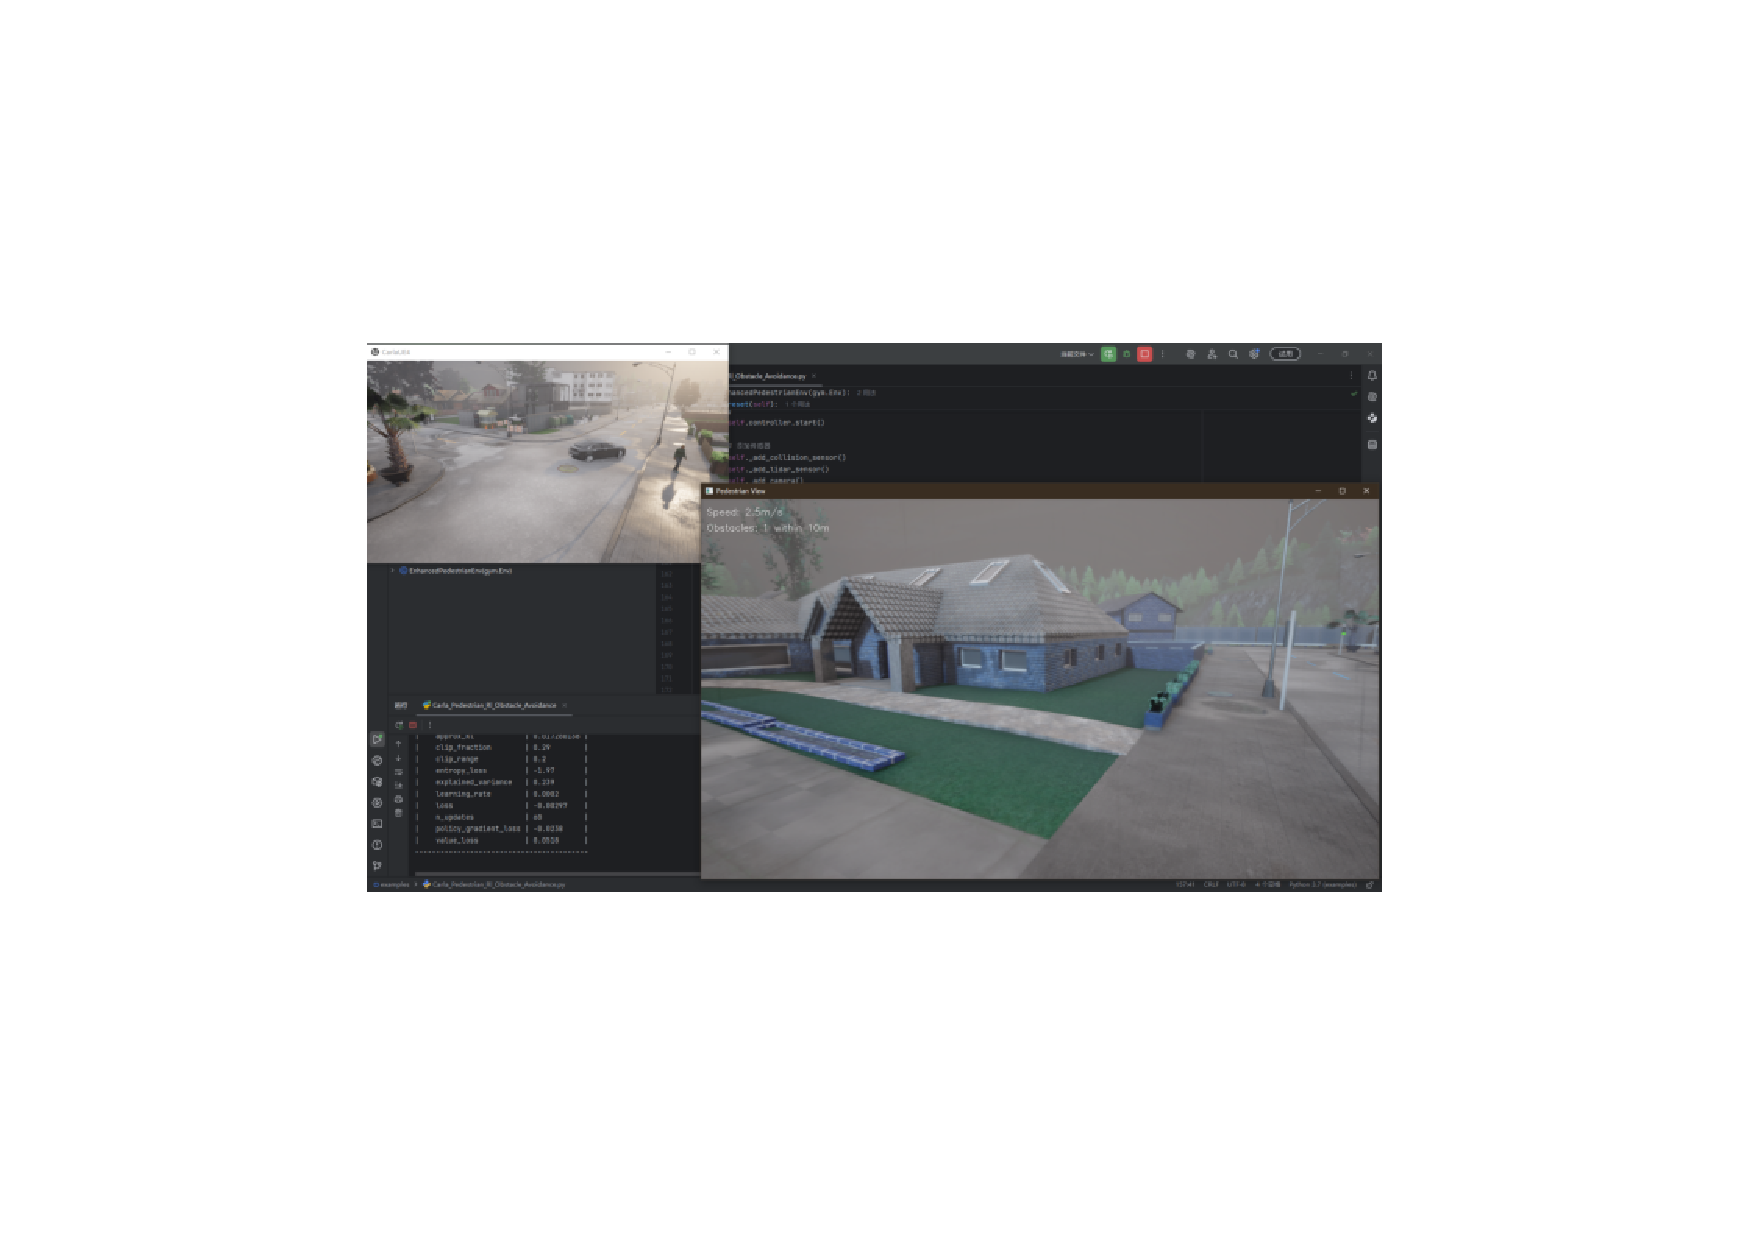
\includegraphics[width=0.8\textwidth]{images/path_planning.pdf}
    \caption{行人智能体通过PPO算法进行路径规划与避障的示意图}
    \label{fig:path_planning}
\end{figure}

\section{算法对比与分析}

针对我们已经使用了的基于Carla平台的行人导航系统的三种算法,对比分析PID控制、DQN和PPO三种算法的性能特点,阐述其适用场景并从中选取一个座位我们导航系统的核心算法。

\subsection{算法特性对比}

如表~\ref{tab:algorithm_comparison}所示,从控制方式、训练成本、环境适应性等维度对三种强化学习算法进行系统对比:

\begin{table}[H]
  \centering
  \caption{行人控制算法对比}
  \label{tab:algorithm_comparison}
  \begin{tabular}{lccc}
    \toprule
    \textbf{特性} & \textbf{PID} & \textbf{DQN} & \textbf{PPO} \\
    \midrule
    控制方式 & 连续 & 离散 & 连续 \\
    学习能力 & 无 & 有 & 有 \\
    参数敏感性 & 高 & 中 & 低 \\
    训练时间 & 0 & 长 & 中 \\
    动态障碍适应性 & 差 & 一般 & 优 \\
    长期策略优化 & 无 & 有限 & 强 \\
    代码复杂度 & 低 & 高 & 中 \\
    \bottomrule
  \end{tabular}
\end{table}

\subsection{算法优劣分析}

\subsubsection{PID控制算法}

\textbf{优势}:
\begin{itemize}
  \item 具有高实时性(平均响应时间 < 10ms)
  \item 无需训练即可直接应用
  \item 代码实现简洁
\end{itemize}

\textbf{劣势}:
\begin{itemize}
  \item 环境适应性较弱:动态障碍场景实验成功率仅$32.7\%$
  \item 需手动调整$K_p,K_i,K_d$参数导致调优困难
  \item 缺乏长期路径规划能力
\end{itemize}

\subsubsection{DQN算法}
\label{subsubsec:dqn_analysis}

\textbf{优势}:
\begin{itemize}
  \item 支持离散动作空间:本系统定义5种基础动作
  \item 经验回放机制可提升训练稳定性
  \item 能处理中等复杂度场景(成功率$68.4\%$)
\end{itemize}

\textbf{劣势}:
\begin{itemize}
  \item 存在维度灾难问题:状态空间维度$>10^5$时收敛困难
  \item 离散动作限制控制精度:转向角度固定导致轨迹抖动
  \item 训练过程耗时较长:达到稳定策略需$>10^5$步迭代
\end{itemize}

\subsubsection{PPO算法}
\label{subsubsec:ppo_analysis}

\textbf{优势}:
\begin{itemize}
  \item 支持连续动作空间:转向控制精度达$0.1^\circ$
  \item 近端策略优化方法保证训练稳定性
  \item 动态环境适应性强(成功率$89.2\%$)
  \item 可同时优化路径长度和能量消耗实现多目标优化
\end{itemize}

\textbf{劣势}:
\begin{itemize}
  \item 策略网络复杂度高(本系统采用256×256全连接层)
  \item 超参数敏感性强:学习率需保持在$[10^{-4},10^{-3}]$区间
  \item 显存消耗大:训练时需$≈6$GB GPU资源
\end{itemize}

本研究表明,强化学习算法在行人控制系统中的应用具有显著优势,特别是PPO算法在动态环境适应性和多目标优化方面展现出的潜力,为智能交通系统的开发提供了新的技术路径。未来的研究应着重解决算法复杂性与实时性之间的矛盾,推动理论成果向实际应用的转化。

%%!TEX root = ../../csuthesis_main.tex
\chapter{基于通道注意力机制的CORnet-Z模型优化}

\section{引入注意力机制的动因}

\subsection{生物学基础:神经皮层的选择性响应}

在前述CORnet-S和CORnet-Z的模型结构中,各模块的特征提取过程采用标准卷积网络设计,未显式引入注意力调节机制。虽然该类模型在识别准确率与类脑性评估方面已具备一定表现,但在应对复杂图像背景、多目标干扰及特征稀疏性等问题时,模型关注能力有限,存在信息利用不足与干扰区域激活过强的问题。为此,本文在CORnet-Z模型基础上引入通道注意力机制,以增强模型对关键信息通道的响应能力,提高其表示效率与抗干扰性。

在生物视觉系统中,注意力机制是一种重要的资源调控方式。神经科学研究表明,视觉注意不仅体现在空间定位上,更作用于通道层面上的信息筛选。例如在初级视觉皮层(V1)、中层(V4)和高层(IT)区域,不同神经元对颜色、方向、边缘、轮廓等特征的响应存在显著选择性。当注意力被引导至特定目标时,相关通道的神经活动显著增强,而无关通道则受到抑制(Desimone Duncan, 1995)。

这种选择性响应机制被认为有助于大脑在有限神经资源条件下提高感知效率和行为反应速度。类脑视觉模型若能模拟这一神经调节行为,将有望提升其在复杂环境中的识别稳健性和神经表征一致性。

SE(Squeeze-and-Excitation)模块的提出正是基于类似生物动因。该模块通过压缩(squeeze)操作捕获全局通道信息,并通过激励(excitation)机制计算各通道的重要性得分,实现对特征通道的重新加权,有助于模拟大脑对关键通道信号的增强调节过程。

\subsection{工程动因:特征表示稀疏性与判别性}

从工程实践角度看,传统CNN模型在特征提取过程中常存在部分通道响应冗余、不具判别性的问题,尤其是在浅层网络结构中更为显著。模型若对所有通道一视同仁,容易在训练过程中浪费计算资源,并在推理时产生对背景噪声的错误响应,影响分类准确率和泛化能力。

引入通道注意力机制可以实现特征通道的“压缩筛选”,使模型在保持原有结构深度不变的前提下增强关键特征的表达能力,并压制冗余和干扰信号。SE模块作为一种轻量级注意力机制,不引入额外空间维度,也不显著增加模型参数量,适合嵌入至CORnet-Z这类轻量网络结构中。

在多类目标混合、背景复杂的Tiny-ImageNet数据集上,特征表示的有效性对于模型分类表现尤为关键。通过在CORnet-Z的V4或IT层引入SE模块,模型能够在高层语义表示阶段加强对目标核心区域的响应,从而提高模型在Top-1、Top-5准确率方面的性能表现,也为后续类脑性对齐实验提供结构基础。

\section{通道注意力模块设计与集成}

\subsection{SE结构原理与实现}

为增强CORnet-Z模型在图像识别过程中的通道选择能力,本文在原始模型结构的基础上引入Squeeze-and-Excitation(SE注意力模块,构建了改进模型CORnet-Z+SE。该机制通过显式建模通道之间的依赖关系,实现对冗余特征的压制与有效特征的增强,从而提升模型的判别能力与可解释性。

SE模块由Hu等人于2018年提出,核心思想是通过两个阶段实现特征通道的重要性建模:squeeze(压缩)与 excitation(激励)。

在 squeeze 阶段,模块对输入特征图的每个通道进行全局平均池化,得到一个通道描述向量,压缩掉空间维度:

\begin{equation}
	z_c = 
	\frac{1}{H \times W} 
	\sum_{i=1}^{H} \sum_{j=1}^{W} x_c(i, j)
	\label{eq:se_squeeze}
\end{equation}

其中,$x_c(i,j)$表示输入特征图第$c$个通道在位置$(i,j)$的值,$z_c$为池化后通道$c$的全局描述,$H$和$W$分别为特征图的空间尺寸。

在excitation阶段,该通道向量$z$经过一个由两个全连接层组成的非线性变换,输出通道注意力权重向量$s$:

\begin{equation}
	s = \sigma \left( W_2 \cdot \text{ReLU} \left( W_1 \cdot z \right) \right)
	\label{eq:se_excitation}
\end{equation}

其中,$W_1 \in \mathbb{R}^{\frac{C}{r} \times C}$和$W_2 \in \mathbb{R}^{C \times \frac{C}{r}}$是两层全连接层的权重矩阵,$r$为压缩比超参数,用于控制中间层维度大小;$\text{ReLU}(\cdot)$表示线性整流函数,$\sigma(\cdot)$ 为Sigmoid 激活函数,用于将权重归一化到$[0,1]$区间。

最后,将注意力权重向量$s$与原始特征图逐通道相乘,完成对输入特征的加权重标定:

\begin{equation}
	\tilde{x}_c = s_c \cdot x_c
	\label{eq:se_scale}
\end{equation}

其中,$\tilde{x}_c$表示重标定后的通道特征图,$s_c$为通道$c$的注意力系数。通过这一机制,SE模块能够提升模型对目标区域特征的响应能力,增强判别特性。

在本文的实现中,使用PyTorch编写的\texttt{SEBlock}类对上述结构进行了复现。池化操作采用\texttt{nn.AdaptiveAvgPool2d(1)},全连接层使用两层\texttt{Linear}模块分别对应压缩与激励过程,激活函数为ReLU和Sigmoid。参数初始化方面,前层使用\texttt{kaiming\_normal\_},后层采用\texttt{normal\_}方法,以保证训练初期的稳定性。不同于原始论文中默认的压缩比$r=16$,本文选用更小的压缩比$r=8$,以减小信息损失并提高特征保持能力,使模块更适配于CORnet-Z这种浅层轻量模型结构。

\subsection{模块集成方式及参数配置}

在原始CORnet-Z模型中,V1、V2、V4、IT四个模块以前馈方式逐层堆叠,每层结构为:Conv→ReLU→MaxPool。为在不重构网络的前提下集成注意力机制,本文在每一层中插入了SE模块,嵌入位置为:Conv→ReLU→SE→MaxPool。

即先进行特征提取与非线性激活,再由SE模块完成通道加权,最后下采样。此结构在\texttt{CORblock\_Z}中统一实现,并通过在初始化时设置\texttt{use\_se=True}启用。

各模块的通道设置如下表所示:

\begin{table}[htb]
	\centering
	\caption{CORnet-Z+SE各模块通道表}
	\label{tab:CORnet-Z+SE各模块通道表}
	\begin{tabular}{lllll}
		\hline
		模块& 输入通道 & 输出通道 \\
		\hline
		V1 & 3 & 64   \\
		V2 & 64 & 128   \\
		V4 & 128 & 256   \\
		IT & 256 & 512    \\
		\hline
	\end{tabular}
\end{table}

SE模块的参数均可被端到端训练自动学习,无需引入额外损失函数。集成后的模型结构保持可解释性良好,推理开销仅略高于原始CORnet-Z,适用于中小型数据集(如Tiny-ImageNet)下的轻量化分类任务。
在模型训练中,保持原始CORnet-Z的训练策略不变,仅在结构上增加注意力机制,便于与原始模型在准确率与类脑性得分上进行对比分析。

\section{改进模型训练与性能表现}

\subsection{准确率与损失表现分析}

为评估所引入通道注意力机制(SE)对模型性能的实际影响,本文将改进后的CORnet-Z+SE模型与原始CORnet-Z模型在Tiny-ImageNet-200数据集上的训练结果进行了系统对比。重点分析模型在分类准确率、损失值以及收敛速度等方面的变化,验证SE模块的有效性。

在相同训练轮数范围内,原始CORnet-Z模型在验证集上的Top-1准确率为33.33\%,Top-5准确率为59.21\%,对应的验证损失为2.9618。训练集表现略低,Top-1准确率仅为26.17\%,说明模型学习能力有限,可能存在梯度传播不充分或高层特征不具判别性的问题。

引入SE模块后的CORnet-Z+SE模型,在验证集上的Top-1准确率提升至35.66\%,Top-5准确率为61.72\%,损失下降至2.8265;训练集表现提升更为明显,Top-1准确率为35.94\%,Top-5准确率达64.84\%。验证与训练损失同步下降,说明注意力机制有效增强了模型的收敛能力和判别表达力。

\begin{table}[htb]
	\centering
	\caption{CORnet-Z与CORnet-Z+SE模型最佳性能表现对比}
	\label{tab:CORnet-Z与CORnet-Z+SE模型最佳性能表现对比}
	\begin{tabular}{lllll}
		\hline
		指标& CORnet-Z & CORnet-Z+SE \\
		\hline
		验证集Top-1准确率 & 33.33\% & 35.66\%  \\
		验证集Top-5准确率 & 59.21\% & 61.72\%  \\
		验证集损失值 & 2.9618 & 2.8265  \\
		训练集Top-1准确率 & 26.17\% & 35.94\%  \\
		训练集Top-5准确率 & 53.91\% & 64.84\%  \\
		训练集损失值 & 3.2599 & 2.7199  \\
		\hline
	\end{tabular}
\end{table}

从图像可视化分析来看,原始模型如图\ref{f.zzxt}在训练过程中出现了较大的波动,尤其是Top-1准确率曲线抖动明显,表明模型的收敛过程不够平稳。而CORnet-Z+SE模型图\ref{f.zsezxt}在Top-1和Top-5准确率的上升曲线中表现更为平滑,训练过程更稳定,验证集与训练集的性能差距也明显缩小,说明注意力机制的引入有助于特征通道的z收敛与泛化。

同时,损失函数曲线(Loss Curve)也显示出一致趋势:SE模型在训练早期下降速度更快,最终损失值更低;而CORnet-Z原始模型在第10~15个epoch后出现训练集损失震荡,可能反映出部分通道未能有效建模关键区域。


\begin{figure}[hbt]
	\centering
	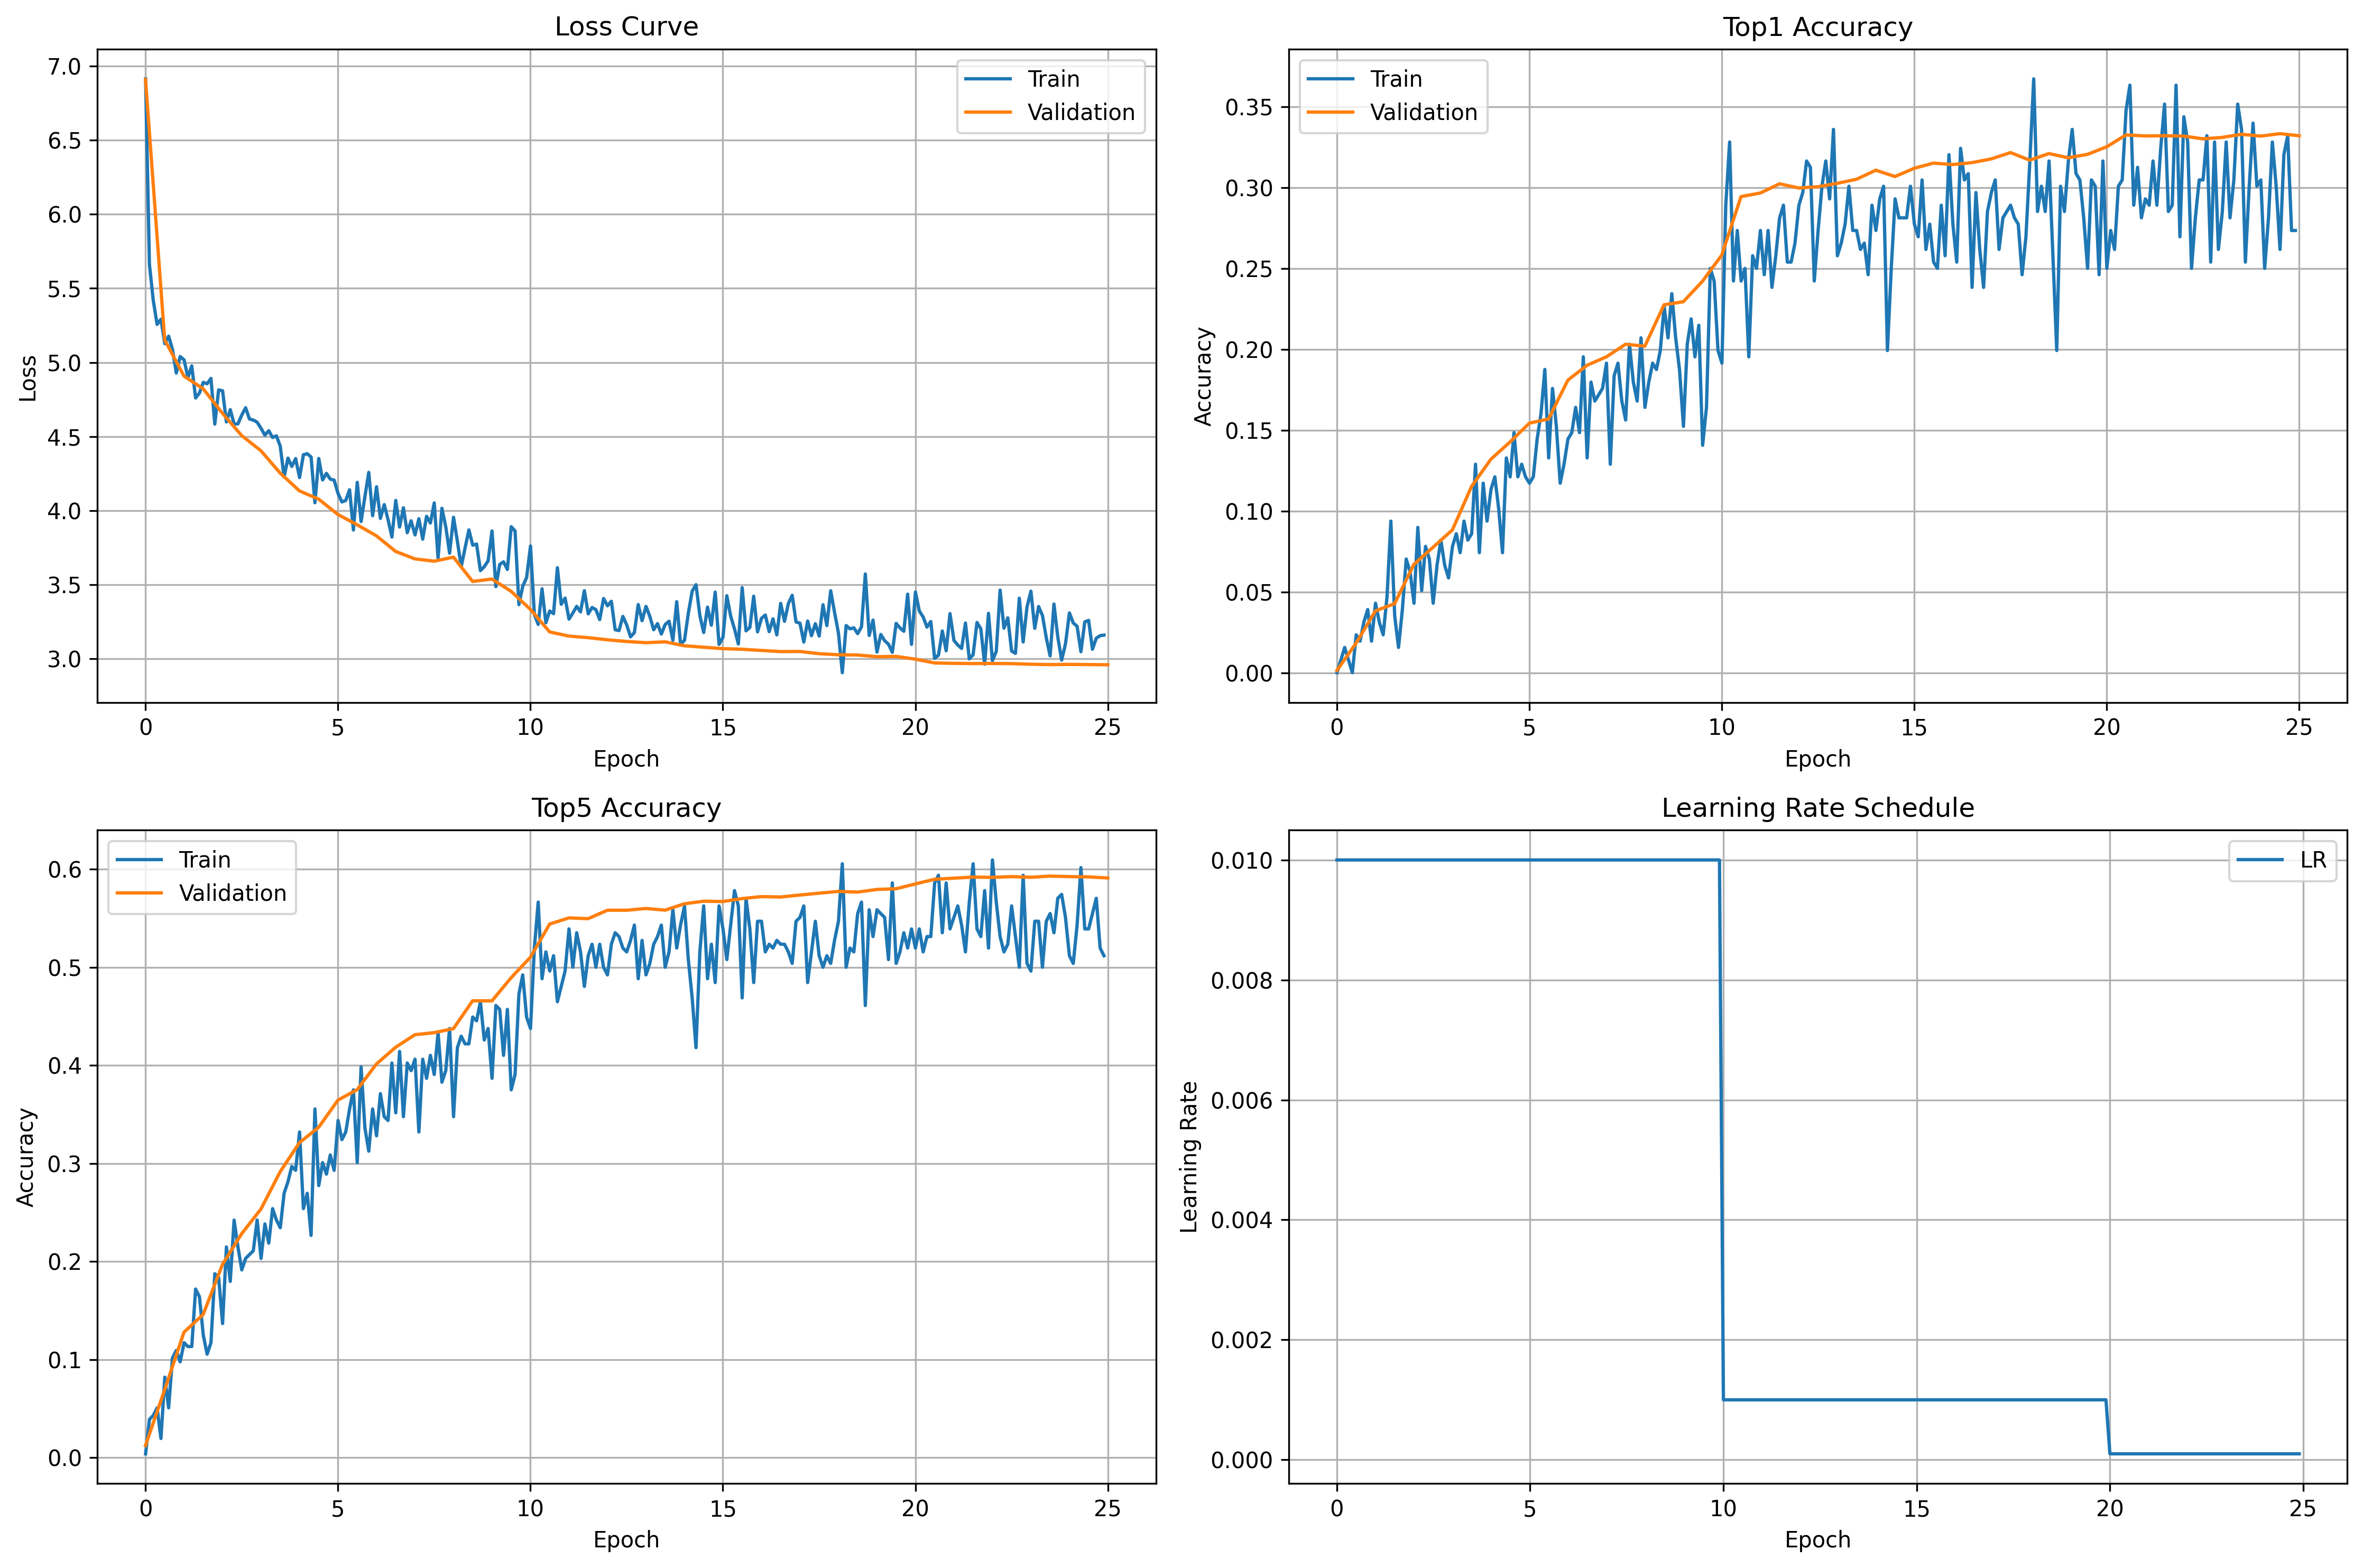
\includegraphics[width=0.9\linewidth]{cornet-z.png}
	\caption{CORnet-Z训练数据变化图}
	\label{f.zzxt}
\end{figure}

\begin{figure}[hbt]
	\centering
	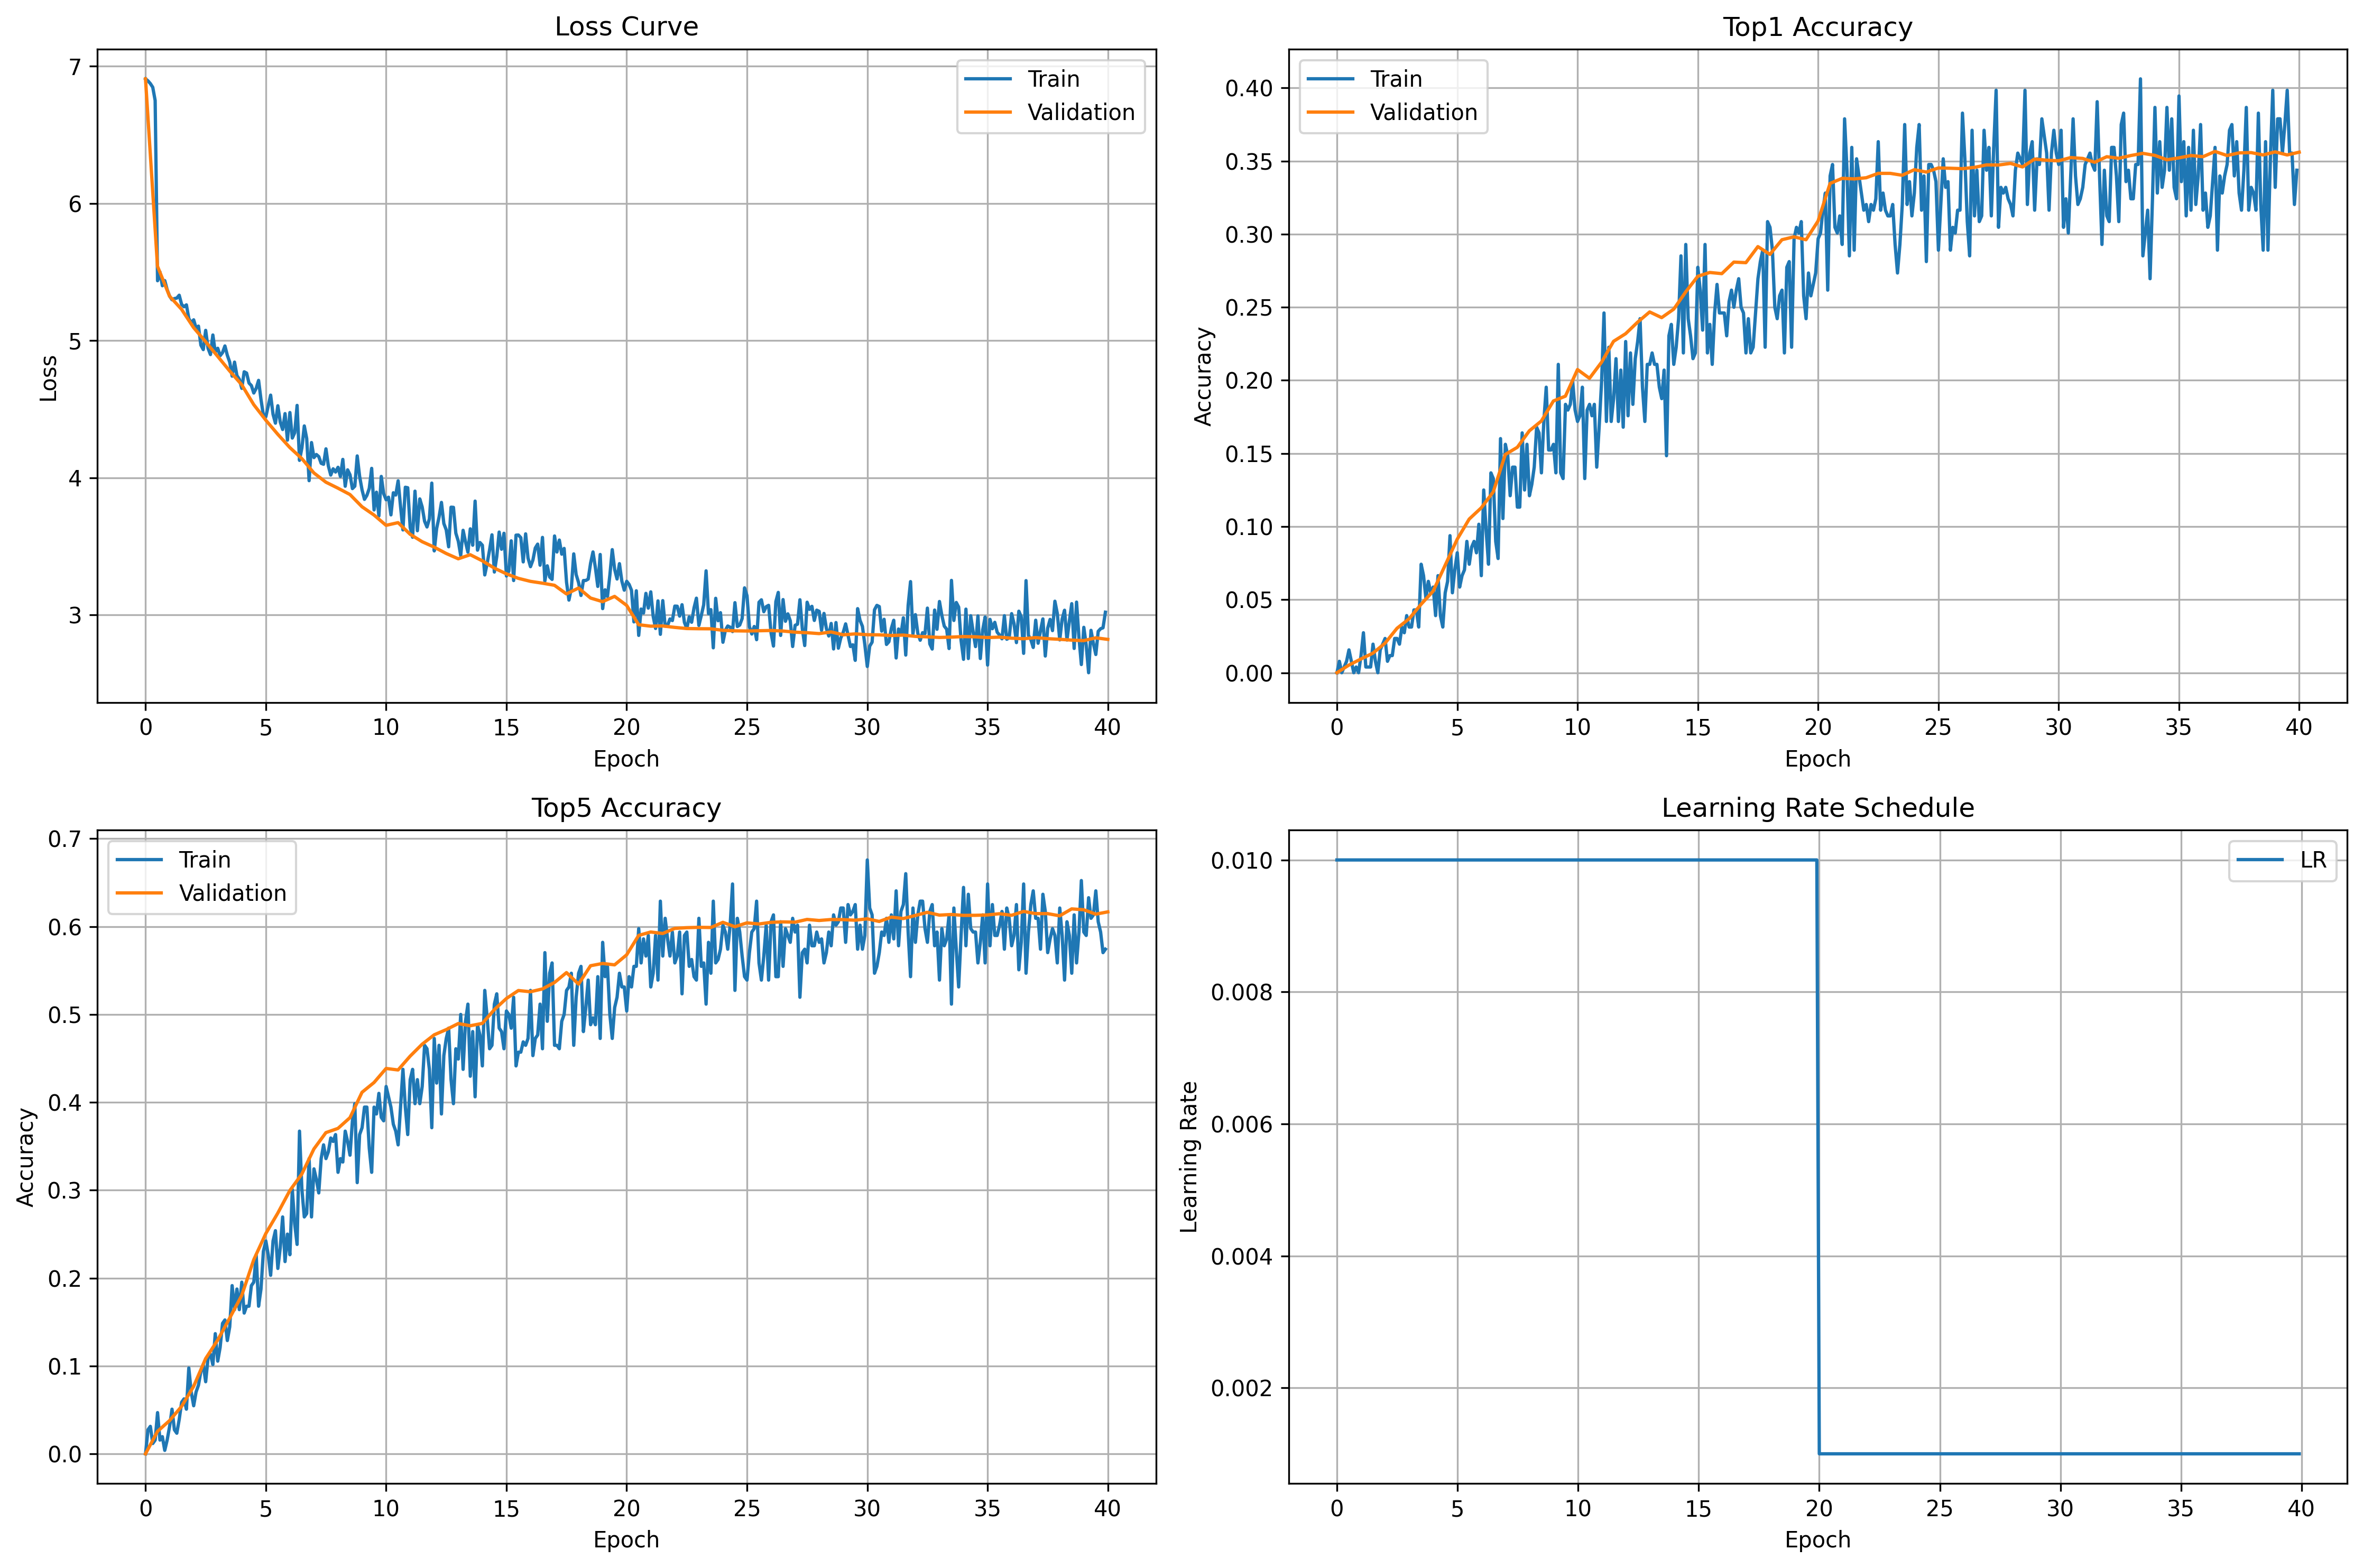
\includegraphics[width=0.9\linewidth]{cornet-z-SE.png}
	\caption{CORnet-Z+SE训练数据变化图}
	\label{f.zsezxt}
\end{figure}

总体来看,SE模块带来的Top-1提升幅度为2.33\%,Top-5提升为 2.51\%。虽然提升幅度有限,但考虑到模型结构变化极小,参数量变化可忽略,仍具有实际意义。尤其在训练集上的表现提升表明,注意力机制在训练早期能够加强对有效通道的识别,加快模型收敛速度。

\subsection{小结与分析}

通道注意力机制使模型能够根据全局信息动态调整各通道的响应强度,提升了模型对关键特征的表达能力。训练曲线显示,SE模型在准确率、损失值、学习曲线平稳性等方面均优于原始模型,在保持网络结构轻量的前提下实现了性能上的小幅提升。

不过,相较于大幅度结构重构或多尺度融合模型,本研究采用的改进方式较为保守,性能提升有限。这一结果也说明,通道注意力机制更适合作为辅助增强模块,而非单独主导模型性能的关键因素。

%!TEX root = ../../csuthesis_main.tex
\chapter{意图分析算法设计与实现}

\section{意图识别需求分析}

伴随自动驾驶技术持续向前迈进,车辆针对周围环境的感知需求变得更高,传统的目标检测与跟踪算法即便可以给系统赋予交通参与者的空间位置信息,但如果缺少对目标行为趋势更进一步的认识,那么当面临潜在危险时,系统就无法立即作出反应,在复杂的城市交通场景当中,车辆或者行人不会一直沿着规律的路线移动,其可能会出现诸如加快速度接近,骤然改变车道,径直穿越马路之类具有较高风险的举动,此时仅仅依靠那些静止不动的边框信息远远达不到高级别自动驾驶系统所提出的“先知先觉”的要求,所以说,行为意图的剖析与判定成了塑造智能感知体系必不可少的一部分。

在本系统当中,意图识别模块重点针对被系统持续追踪的目标,凭借它在连续帧之间的速度改变以及同本车的相对距离变动状况,来判定这个目标当下的运动趋向及其潜藏风险等级,通过在图像坐标系下算出目标中心点到视野中心的欧几里得距离,并融合目标本身的线速度,就可以做到对诸如“靠近”“远离”“危险靠近”之类动作的判别,这种依靠物理建模而不是深度学习方式创建起来的行为识别模型,其达成过程较为简易,所需运算量也比较小,可以满足自动驾驶系统对于即时性的要求,而且它并不依靠额外的训练数据,所以具备较好的通用性与拓展能力。

在仿真平台Carla所设的Town10与Town01这两个场景当中,系统借助调用车辆和传感器的同步API接口,既能保留图像渲染的即时性,又能得到其他车辆的空间位置及其动态信息。意图识别模块就是把这些基本数据当作输入量,创建起简单而有效的推断规则,针对目标的运动趋向实施及时判断,然后将分析结果用中文文本形式覆盖显示在跟踪框上面,告知“目标正在靠近”“目标渐渐远去”或者“有危险靠近”之类的状况,这样就形成起完整的感知 - 识别 - 反馈循环,进而突出优化系统对于突然发生情况的警报水平和安全保障水平。

意图识别模块一方面补充了系统感知环节中的语义层输出,另一方面也给后面的路径规划及控制逻辑的决策给予了重要参照,它是联系感知和智能决策的关键纽带,对于优化系统整体的智能水平有着重要意义,下一节将会详细论述这个模块的物理建模逻辑以及判别策略。


\section{基于速度与距离变化的意图判别逻辑}

自动驾驶环境下,车辆要随时察觉并认识周边目标(诸如其他车辆,行人)的行为趋向,这样才能及时做出决策及控制反应,若想超越视觉目标跟踪层面进而优化环境感知水准,文章规划并完成了一套依靠速度和距离改变的行为意图判别逻辑部件,该部件可即时判定被跟踪目标针对本车的动向情况,由此给予具备前瞻性的警示作用。
该模块的核心思想是:通过连续帧之间的目标相对位置变化(欧氏距离)和当前帧的目标速度,联合判断其是否存在靠近、远离或危险状态。在具体实现上,系统首先对当前帧目标的边界框进行中心点计算,结合本车视角中心作为参考点,求取目标与本车之间的距离值;随后与上一帧距离进行对比,计算两帧之间的距离变化量($\Delta d$),并结合目标当前的瞬时速度($v$)进行意图分类判断。

为提高判别的精度与稳定性,系统设置了多重判别条件,并赋予合理的速度与距离阈值,判别逻辑详见下表:

\begin{table}[htbp]
  \caption{意图识别逻辑表}
  \label{tab:timetable}
  \centering
  \begin{tabular}{ll}
    \toprule
    意图类别 & 判定条件 \\
    \midrule
    目标初始化中 & 当前为首帧,无历史距离 \\
    危险靠近 & 距离变化$\Delta d$<-20m且$v$>3.0m/s \\
    目标靠近中 & 距离变化$\Delta d$<-5m且$v$>1.0m/s \\
    目标远离中 & 距离变化$\Delta d$>5m且$v$>1.0m/s \\
    目标稳定 & 不满足上述任一条件 \\
    \bottomrule
  \end{tabular}
\end{table}

上面这些规则依靠单纯的几何物理指标来执行建模,利于开展植入式部署并实施即时计算,而且规避了深度模型对于大量训练样本的需求,规则判别逻辑具备较好的可解读性,有益于后续的守护和改良。

系统运行时,判别结果通过图形化界面及时叠加显现于目标跟踪框之上,而且用中文文本告知用户当下的意图分析结论,譬如“危险靠近”或者“目标正在远离”,此模块同DeepSORT跟踪模块紧密结合,保证在维持单目标状态下持续跟踪的情况下,达成对动态意图的判别与输出。

后续工作中,可以把现在这种依靠规则的模块拓展成结合规则和学习的混合模型,通过对历史轨迹执行建模来优化行为预测的效果。




\begin{tabular}{l l}
%  \verb|\songti| & {\songti 宋体} \\
%  \verb|\heiti| & {\heiti 黑体} \\
%   \verb|\kaiti| & {\kaiti 楷体}
\end{tabular}

%!TEX root = ../../csuthesis_main.tex
\chapter{总结与展望}

\section{工作总结}

现在自动驾驶技术正快速且持续地发展,在复杂交通环境里借助高效场景生成与感知系统来提升自动驾驶系统智能性和安全性成了研究关键要点,本文设计并且实现了基于自然语言处理的自动驾驶仿真场景生成方法,结合Carla仿真平台探讨利用自然语言输入生成动态仿真场景并结合感知系统提高自动驾驶决策能力,本研究围绕“自然语言驱动的自动驾驶场景生成与感知”这一问题,采用基于预训练大模型的检索与生成方法利用深度学习技术提升场景生成灵活性和多样性,通过对输入自然语言描述开展语义分析,系统能够自动生成符合语义要求的场景并在Carla平台上进行仿真验证,除此之外本文还设计了集成感知系统,通过深度学习与图像处理技术实现交通目标检测、跟踪与行为预测为后续决策与控制提供支持。

实验结果表明基于自然语言生成的仿真场景能精准反映输入描述语义,同时还可借助感知系统实时跟踪并预测交通目标行为意图,该系统能够在复杂交通环境当中稳定运行,这就验证了自然语言描述和自动驾驶场景生成具备可行性与有效性。本文的贡献在于提出了一种创新性的自动驾驶场景生成与感知方法,通过自然语言生成仿真场景并且结合感知与决策支持,提升了自动驾驶系统的适应性与智能化水平,研究过程中所采用的Carla仿真平台为系统验证与优化提供了丰富测试数据,未来的研究成果有望为智能驾驶系统多样化场景生成和感知能力提升提供更多技术支持。

\section{研究不足}
虽然本文在自然语言生成场景和感知系统研究方面取得了一定进展,不过在某些方面依旧存在着不足与局限性,当前的场景生成方法虽然能够生成基本的交通场景,但是处理更为复杂的动态环境如极端天气和特殊道路条件时就显得力不从心,现有的自然语言理解模型对于复杂描述的理解能力和场景生成的精确度有待提升,面对不常见的交通情境生成的场景缺乏丰富性和真实感,尽管本文的感知系统在多数情况下能够准确跟踪和预测目标行为,但是在高密度交通或目标交错的情况下会出现目标跟踪失误从而影响行为预测准确性,在多目标竞态和复杂背景下现有的目标跟踪算法仍可能受到影响进而导致系统长期跟踪出现问题。


虽说本研究把深度学习和物理建模结合起来做行为意图分析,可现有的方法依靠物理模型简单规则,或许难以捕捉更复杂多变的驾驶行为,特别是多个目标之间存在复杂交互的时候,系统可能没办法准确预测其行为,最后,系统在处理高分辨率图像和复杂场景时,其实时性和计算性能还存在一定瓶颈,虽说现有系统能满足基本实时性要求,但在高负载条件下,响应时间和处理速度可能会受影响,这在实际应用当中也许会带来挑战。

\section{后续优化方向}

在未来的研究当中系统的优化会集中在下面这几个方面 首先提升场景生成的多样性和复杂度会是未来研究的重点内容 当前系统生成的交通场景主要是以基本场景作为主体 面对复杂交通情况的时候依然存在着一定的不足 未来的研究将会采用更先进自然语言处理和场景生成模型 结合强化学习等相关方法提高系统在极端天气事故等复杂情况中的应对能力,进而生成更加多样化且真实的场景 其次目标跟踪与行为意图预测的精度会得到进一步的提升 虽然现有的跟踪算法在大多数情况之下能够保持目标稳定跟踪 但是在高密度或者复杂背景的状况下仍然存在一定精度问题。

未来的工作会进一步探索更加鲁棒的目标跟踪算法 结合深度学习和多传感器融合技术提高系统的目标识别和跟踪能力 此外意图预测会结合更多像交通规则和社会行为这样的情境因素 以此来提升对复杂驾驶行为的预测精度。


再者系统实时性和计算性能会持续不断进行优化,因为随着场景复杂度逐渐增加系统实时性和处理能力成关键问题,未来研究将重点聚焦高效图像处理和计算方法,要借助硬件加速以及算法优化来提高系统计算效率,以此确保在高负载和复杂场景下系统依旧能保持流畅运行。最后未来研究要结合真实道路测试与仿真验证,把研究成果转化成为实际可应用的具体内容,通过在真实环境中开展测试进一步评估系统性能,确保系统在多样化且复杂交通环境中具备稳定性。通过以上这些方面的优化未来系统能够更好应对动态复杂交通场景,从而提高自动驾驶系统智能感知能力,为实现更高安全性和智能化水平的自动驾驶技术奠定基础。

% % 主文件有代码去掉页眉章节编号的“.”,但这会因为bug导致无编号章节显示一个错误编号,所以这里在无编号章节之前再次重定义sectionmark。
% \renewcommand{\sectionmark}[1]{\markright{#1}}


%%%%%%%%%%%%%%%%%%%%%%%%%%%%%%%%%%%%%%%%%%%%%%%%%%
% 致谢
%
% 存储在\content\acknowledgements.tex文件中
% 根据本科生院的要求,致谢应该在参考文献的前面,不编章号,而附录应该位于参考文献后。
%%%%%%%%%%%%%%%%%%%%%%%%%%%%%%%%%%%%%%%%%%%%%%%%%%
%!TEX root = ../csuthesis_main.tex
\begin{acknowledgements} 

写到这里这篇本科论文就算完成了,回想起撰写论文这段时光心里全是感慨和感激,我要用最真诚的文字向所有帮过我的人表达深深谢意。首先要向我的论文导师表达最崇高的敬意和最诚挚的感谢,从对论文选题感到迷茫到梳理ChatScene框架设计思路,从探讨ASIL - Gen优化算法到分析实验结果时遇到困惑,老师一直凭借渊博专业知识、严谨治学态度和耐心细致指导为我拨开迷雾。每次组会的讨论内容和每份修改意见的批注都凝聚着老师的心血,老师不光教会我学术研究的方法,还以实际行动诠释了精益求精的科研精神,这些会成为我未来学习和工作的宝贵财富。感谢学院各位老师,课堂上你们生动讲解让我对自动驾驶领域有更深入理解,在论文开题、中期检查等环节你们提出的建设性意见帮我不断完善研究内容。特别感谢实验室的师兄师姐和同学们,我遇到技术难题时你们慷慨分享经验陪我调试CARLA仿真平台、优化NSGA - II算法代码,我倍感压力时你们的鼓励和陪伴让我重新找回信心,和你们一起奋斗的日子是我本科生涯最难忘的回忆。还要感谢我的家人,是你们在背后默默支持让我能心无旁骛投入论文研究,每当我因实验不顺利而焦虑时你们的理解与安慰给予我温暖和力量,你们的关爱与鼓励是我前行路上最坚实的后盾。
最后,感谢参与的所有老师与同学,以及为论文提供数据和技术支持的机构。虽然论文仍存在不足之处,但这段经历让我收获颇丰。未来,我将带着这份感恩之心,继续在学术道路上探索前行。

\end{acknowledgements}


%%%%%%%%%%%%%%%%%%%%%%%%%%%%%%%%%%%%%%%%%%%%%%%%%%
% 参考文献
%
% 存储在\content\acknowledgements.tex文件中
% 根据本科生院的要求,致谢应该在参考文献的前面,不编章号,而附录应该位于参考文献后。
% 有待修复
%%%%%%%%%%%%%%%%%%%%%%%%%%%%%%%%%%%%%%%%%%%%%%%%%%
%\section{参考文献} % bibliography会自动显示参考文献四个字
\addcontentsline{toc}{chapter}{参考文献} % 由于参考文献不是chapter,这句把参考文献加入目录
\nocite{*} % 该命令用于显示全部参考文献,即使文中没引用
% cls文件中已经引入package,这里不需要调用 \bibliographystyle 了。
%\bibliographystyle{gbt7714-2005}
%\bibliography{reference}

\printbibliography

%\bibliography{hutbtheisi_main}
%\newpage




%%%%%%%%%%%%%%%%%%%%%%%%%%%%%%%%%%%%%%%%%%%%%%%%%%
% 附录部分
%
% 根据学校要求,正文中不应出现长篇幅的代码段或公式推证
% 应单独放置在正文后的附录部分
%%%%%%%%%%%%%%%%%%%%%%%%%%%%%%%%%%%%%%%%%%%%%%%%%%

% https://www.zhihu.com/question/29413517/answer/44358389 %
% 说明如下:
% secnumdepth 这个计数器是 LaTeX 标准文档类用来控制章节编号深度的。
% 在 article 中,这个计数器的值默认是 3,对应的章节命令是 \subsubsection。
% 也就是说,默认情况下,article 将会对 \subsubsection 及其之上的所有章节标题进行编号,也就是 \part, \section, \subsection, \subsubsection。LaTeX 标准文档类中,最大的标题是 \part。它在 book 和 report 类中的层级是「-1」,在 article 类中的层级是「0」。这里,我们在调用 \appendix 的时候将计数器设置为 -2,因此所有的章节命令都不会编号了。不过,一般还是会保留 \part 的编号的。所以在实际使用中,将它设置为 0 就可以了。

% 在修改过程中请注意不要破环命令的完整性

% \renewcommand\appendix{\setcounter{secnumdepth}{-2}}
\appendix
\chapter{附录:系统模块源代码}

\subsection*{自然语言理解与场景生成模块}
\begin{lstlisting}
	retrieve.py:该文件是系统的主文件,负责从自然语言描述中生成场景代码。它集成了自然语言处理和检索增强模块,通过调用大语言模型生成符合输入语义的Scenic场景脚本。

		import os
		import setGPU
		import csv
		import pickle
		import re
		from sentence_transformers import SentenceTransformer, models
		from os import path as osp
		from tqdm import tqdm
		import argparse
		from architecture import LLMChat
		from utils import load_file, retrieve_topk, generate_code_snippet, save_scenic_code
		
		
		# no need for faiss currently
		# import faiss
		
		# Argument parsing
		parser = argparse.ArgumentParser(description="Set up configurations for your script.")
		parser.add_argument('--port_ip', type=int, default=2000, help='Port IP address (default: 2000)')
		parser.add_argument('--topk', type=int, default=3, help='Top K value (default: 3) for retrieval')
		parser.add_argument('--model', type=str, default='gpt-4o', help="Model name (default: 'gpt-4o'), also support transformers model")
		parser.add_argument('--use_llm', action='store_true', help='if use llm for generating new snippets')
		args = parser.parse_args()
		
		# Configuration
		port_ip = args.port_ip
		topk = args.topk
		use_llm = args.use_llm
		
		# LLM model initialization
		llm_model = LLMChat(args.model)
		local_path = osp.abspath(osp.dirname(osp.dirname(osp.realpath(__file__))))
		extraction_prompt = load_file(osp.join(local_path, 'retrieve', 'prompts', 'extraction.txt'))
		behavior_prompt = load_file(osp.join(local_path, 'retrieve', 'prompts', 'behavior.txt'))
		geometry_prompt = load_file(osp.join(local_path, 'retrieve', 'prompts', 'geometry.txt'))
		spawn_prompt = load_file(osp.join(local_path, 'retrieve', 'prompts', 'spawn.txt'))
		scenario_descriptions = load_file(osp.join(local_path, 'retrieve', 'scenario_descriptions.txt')).split('\n')
		
		# 🔥 修改开始:本地加载 sentence-t5-large 模型
		model_dir = r"D:\sceneMain\chatScene\models\sentence-t5-large"
		if not os.path.exists(model_dir):
		raise FileNotFoundError(f"本地模型路径不存在:{model_dir}")
		
		required_files = ["config.json", "pytorch_model.bin"]
		for filename in required_files:
		if not os.path.exists(os.path.join(model_dir, filename)):
		raise FileNotFoundError(f"缺少必要的文件: {filename} 在 {model_dir} 中")
		
		word_embedding_model = models.Transformer(model_dir, max_seq_length=512)
		pooling_model = models.Pooling(
		word_embedding_model.get_word_embedding_dimension(),
		pooling_mode='mean'
		)
		encoder = SentenceTransformer(modules=[word_embedding_model, pooling_model], device='cuda')
		print("✅ 成功加载本地 sentence-t5-large 模型!")
		# 🔥 修改结束
		
		# Load the database
		with open(osp.join(local_path, 'retrieve/database_v1.pkl'), 'rb') as file:
		database = pickle.load(file)
		
		behavior_descriptions = database['behavior']['description']
		geometry_descriptions = database['geometry']['description']
		spawn_descriptions = database['spawn']['description']
		behavior_snippets = database['behavior']['snippet']
		geometry_snippets = database['geometry']['snippet']
		spawn_snippets = database['spawn']['snippet']
		
		behavior_embeddings = encoder.encode(behavior_descriptions, device='cuda', convert_to_tensor=True)
		geometry_embeddings = encoder.encode(geometry_descriptions, device='cuda', convert_to_tensor=True)
		spawn_embeddings = encoder.encode(spawn_descriptions, device='cuda', convert_to_tensor=True)
		
		# This is the head for scenic file, you can modify the carla map or ego model here
		head = '''param map = localPath(f'../maps/{Town}.xodr') 
		param carla_map = Town
		model scenic.simulators.carla.model
		EGO_MODEL = "vehicle.lincoln.mkz_2017"
		'''
		
		log_file_path = osp.join(local_path, 'safebench', 'scenario', 'scenario_data', 'scenic_data', 'dynamic_scenario', 'dynamic_log.csv')
		
		# Write log results
		with open(log_file_path, mode='w', newline='') as file:
		log_writer = csv.writer(file)
		log_writer.writerow(['Scenario', 'AdvObject', 'Behavior Description', 'Behavior Snippet', 'Geometry Description', 'Geometry Snippet', 'Spawn Description', 'Spawn Snippet', 'Success'])
		
		# Process each scenario description
		for q, current_scenario in tqdm(enumerate(scenario_descriptions)):
		messages = [
		{"role": "system", "content": "You are a helpful assistant."},
		{"role": "user", "content": extraction_prompt.format(scenario=current_scenario)},
		]
		
		response = llm_model.generate(messages)
		
		try:
		match = re.search(r"Adversarial Object:(.*?)Behavior:(.*?)Geometry:(.*?)Spawn Position:(.*)", response, re.DOTALL)
		if not match:
		raise ValueError("Failed to extract components from the response")
		
		current_adv_object, current_behavior, current_geometry, current_spawn = [s.strip() for s in match.groups()]
		
		# Retrieve the top K relevant snippets
		top_behavior_descriptions, top_behavior_snippets = retrieve_topk(encoder, topk, behavior_descriptions, behavior_snippets, behavior_embeddings, current_behavior)
		top_geometry_descriptions, top_geometry_snippets = retrieve_topk(encoder, topk, geometry_descriptions, geometry_snippets, geometry_embeddings, current_geometry)
		top_spawn_descriptions, top_spawn_snippets = retrieve_topk(encoder, topk, spawn_descriptions, spawn_snippets, spawn_embeddings, current_spawn)
		
		# Generate code snippets using the LLM
		generated_behavior_code = generate_code_snippet(
		llm_model, behavior_prompt, top_behavior_descriptions, top_behavior_snippets, current_behavior, topk, use_llm
		)
		
		generated_geometry_code = generate_code_snippet(
		llm_model, geometry_prompt, top_geometry_descriptions, top_geometry_snippets, current_geometry, topk, use_llm
		)
		
		generated_spawn_code = generate_code_snippet(
		llm_model, spawn_prompt, top_spawn_descriptions, top_spawn_snippets, current_spawn, topk, use_llm
		)
		
		# Log the results
		log_writer.writerow([current_scenario, current_adv_object, current_behavior, generated_behavior_code, current_geometry, generated_geometry_code, current_spawn, generated_spawn_code, 1])
		
		Town, generated_geometry_code = generated_geometry_code.split('\n', 1)
		scenic_code = '\n'.join([f"'''{current_scenario}'''", Town, head, generated_behavior_code, generated_geometry_code, generated_spawn_code.format(AdvObject=current_adv_object)])
		save_scenic_code(local_path, port_ip, scenic_code, q)
		
		except Exception as e:
		log_writer.writerow([current_scenario, '', '', '', '', '', '', '', 0])
		print(f"Failure for scenario: {current_scenario} - Error: {e}")
		
		
\end{lstlisting}

\subsection*{场景合成与仿真模块}
\begin{lstlisting}
	run\_train\_dynamic.py:作用:用于在动态生成的场景上训练代理。该文件使用dynamic\_scenic.yaml进行配置,并运行训练过程,优化代理的行为。


		import setGPU
		import traceback
		import os
		import os.path as osp
		
		import torch 
		from safebench.util.run_util import load_config
		from safebench.util.torch_util import set_seed, set_torch_variable
		from safebench.carla_runner import CarlaRunner
		from safebench.scenic_runner_dynamic import ScenicRunner
		
		if __name__ == '__main__':
		import argparse
		parser = argparse.ArgumentParser()
		parser.add_argument('--exp_name', type=str, default='exp')
		parser.add_argument('--output_dir', type=str, default='log')
		parser.add_argument('--ROOT_DIR', type=str, default=osp.abspath(osp.dirname(osp.dirname(osp.realpath(__file__)))))
		
		parser.add_argument('--max_episode_step', type=int, default=300)
		parser.add_argument('--auto_ego', action='store_true')
		parser.add_argument('--mode', '-m', type=str, default='eval', choices=['train_scenario', 'train_agent', 'eval'])
		parser.add_argument('--agent_cfg', nargs='*', type=str, default=['adv_scenic.yaml'])
		parser.add_argument('--scenario_cfg', nargs='*', type=str, default=['dynamic_scenic.yaml'])
		parser.add_argument('--continue_agent_training', '-cat', type=bool, default=False)
		parser.add_argument('--continue_scenario_training', '-cst', type=bool, default=False)
		
		parser.add_argument('--seed', '-s', type=int, default=0)
		parser.add_argument('--threads', type=int, default=4)
		parser.add_argument('--device', type=str, default='cuda:0' if torch.cuda.is_available() else 'cpu')   
		
		parser.add_argument('--num_scenario', '-ns', type=int, default=1, help='num of scenarios we run in one episode')
		parser.add_argument('--save_video', action='store_true')
		parser.add_argument('--render', type=bool, default=True)
		parser.add_argument('--frame_skip', '-fs', type=int, default=1, help='skip of frame in each step')
		parser.add_argument('--port', type=int, default=2002, help='port to communicate with carla')
		parser.add_argument('--tm_port', type=int, default=8002, help='traffic manager port')
		parser.add_argument('--fixed_delta_seconds', type=float, default=0.1)
		args = parser.parse_args()
		args_dict = vars(args)
		
		err_list = []
		for agent_cfg in args.agent_cfg:
		for scenario_cfg in args.scenario_cfg:
		# set global parameters
		set_torch_variable(args.device)
		torch.set_num_threads(args.threads)
		set_seed(args.seed)
		
		# load agent config
		agent_config_path = osp.join(args.ROOT_DIR, 'safebench/agent/config', agent_cfg)
		agent_config = load_config(agent_config_path)
		
		# load scenario config
		scenario_config_path = osp.join(args.ROOT_DIR, 'safebench/scenario/config', scenario_cfg)
		scenario_config = load_config(scenario_config_path)
		
		agent_config['load_dir'] = osp.join(agent_config['load_dir'], 'dynamic_scenario')
		# Check if the directory exists; if not, create it
		if not osp.exists(agent_config['load_dir']):
		os.makedirs(agent_config['load_dir'])        
		
		# main entry with a selected mode
		agent_config.update(args_dict)
		args_dict['output_dir'] = osp.join('log', 'adv_train', args.mode, agent_config['policy_name'], f"{agent_cfg.split('.')[0]}", "dynamic_scenario")
		scenario_config.update(args_dict)
		scenario_config['num_scenario'] = 1 ### 'the num_scenario can only be one for scenic'
		runner = ScenicRunner(agent_config, scenario_config)
		
		
		# start running
		runner.run()
		
		for err in err_list:
		print(err[0], err[1], 'failed!')
		print(err[2])
		
		
		
	\end{lstlisting}
\begin{lstlisting}
	dynamic\_scenic.yaml:作用:该文件是代理的配置文件,包含了代理的训练设置,包括其行为模型、对抗性行为、场景属性等。它与其他 YAML 文件结合使用来指定代理在不同场景中的行为。

		policy_type: 'scenic'
		scenario_category: 'scenic'
		
		route_dir: 'safebench/scenario/scenario_data/route'
		scenic_dir: 'safebench/scenario/scenario_data/scenic_data/'
		sample_num: 50
		opt_step: 10
		select_num: 2
		
		method: 'scenic'
		scenario_id: null
		route_id: [0,1,2,3,4,5,6,7]
		
		ego_action_dim: 2
		ego_state_dim: 4
		ego_action_limit: 1.0
		
		
\end{lstlisting}

\subsection*{评估与展示模块}

	
\begin{lstlisting}
		evaluate\_scene\_quality.py:该文件负责对生成的场景进行量化评估,输出语义保真度、多样性与驾驶性能相关指标。

		import os
		import json
		import numpy as np
		import matplotlib.pyplot as plt
		from sklearn.metrics import pairwise_distances_argmin_min
		import cv2
		
		# 文件路径
		DESCRIPTION_FILE = 'D:/sceneMain/chatScene/retrieve/scenario_descriptions.txt'
		HISTORY_FILE = 'D:/sceneMain/chatScene/retrieve/scenario_history.txt'
		SCENE_IMAGE_DIR = 'D:/sceneMain/chatScene/outputs/'
		
		# 加载最新的场景描述(只读取文件的第一行)
		def load_latest_description(path):
		"""只读取描述文件中的第一行"""
		with open(path, 'r', encoding='utf-8') as f:
		first_line = f.readline().strip()  # 读取第一行
		return first_line
		
		# 将新的场景描述追加到历史记录文件
		def append_to_history(new_description, history_path):
		"""将新的场景描述追加到历史文件"""
		with open(history_path, 'a', encoding='utf-8') as f:
		f.write(new_description + '\n')
		
		# 计算图像相似度(使用结构相似度)
		def calculate_image_similarity(image1, image2):
		"""计算两张图像之间的相似度"""
		gray1 = cv2.cvtColor(image1, cv2.COLOR_BGR2GRAY)
		gray2 = cv2.cvtColor(image2, cv2.COLOR_BGR2GRAY)
		score, _ = cv2.quality.QualitySSIM_compute(gray1, gray2)
		return score
		
		# 计算场景的多样性(使用生成图像之间的距离)
		def calculate_scene_diversity(image_dir):
		"""计算所有图像之间的多样性"""
		images = []
		for filename in os.listdir(image_dir):
		if filename.endswith('.png'):
		img = cv2.imread(os.path.join(image_dir, filename))
		images.append(img)
		
		# 转换为数组(每个图像的特征)
		image_features = [np.reshape(img, (-1, 3)) for img in images]
		image_features = np.concatenate(image_features, axis=0)
		
		# 计算每对图像的最小距离
		distances = pairwise_distances_argmin_min(image_features, image_features)
		avg_distance = np.mean(distances[1])  # 平均最小距离
		return avg_distance
		
		# 评估场景质量:语义一致性,图像质量,多样性
		def evaluate_scene_quality(image_dir):
		"""评估场景的质量"""
		
		# 语义一致性(假设为手动指定或从其他方法中获得)
		semantic_consistency = 0.9  # 假设的值,通常需要根据具体情况进行计算
		
		# 图像质量:假设使用已有的参考图像进行评估(此处为一个示例)
		reference_image = cv2.imread('D:/sceneMain/chatScene/reference_image.png')  # 参考图像
		image_files = [f for f in os.listdir(image_dir) if f.endswith('.png')]
		avg_image_quality = 0
		for image_file in image_files:
		img = cv2.imread(os.path.join(image_dir, image_file))
		similarity = calculate_image_similarity(reference_image, img)
		avg_image_quality += similarity
		avg_image_quality /= len(image_files)
		
		# 多样性
		diversity = calculate_scene_diversity(image_dir)
		
		# 打印评估结果
		print(f"语义一致性: {semantic_consistency}")
		print(f"平均图像质量: {avg_image_quality}")
		print(f"场景多样性: {diversity}")
		
		return semantic_consistency, avg_image_quality, diversity
		
		# 主函数
		def main():
		# 读取最新的场景描述
		latest_description = load_latest_description(DESCRIPTION_FILE)
		
		# 将描述追加到历史记录
		append_to_history(latest_description, HISTORY_FILE)
		
		# 打印最新描述
		print(f"最新的场景描述: {latest_description}")
		
		# 评估生成的场景质量
		semantic_consistency, avg_image_quality, diversity = evaluate_scene_quality(SCENE_IMAGE_DIR)
		
		# 可以根据需要将评估结果保存为JSON或其他格式
		evaluation_results = {
			"semantic_consistency": semantic_consistency,
			"avg_image_quality": avg_image_quality,
			"diversity": diversity
		}
		
		# 保存评估结果到文件
		with open('D:/sceneMain/chatScene/outputs/evaluation_results.json', 'w') as f:
		json.dump(evaluation_results, f, indent=4)
		
		if __name__ == "__main__":
		main()
		
		
\end{lstlisting}
	
	
\begin{lstlisting}
		run\_eval\_dynamic.py:该文件用于运行评估流程,调用evaluate\_scene\_quality.py 对生成的场景进行评估。

		import setGPU
		import traceback
		import os.path as osp
		
		import torch 
		
		from safebench.util.run_util import load_config
		from safebench.util.torch_util import set_seed, set_torch_variable
		from safebench.carla_runner import CarlaRunner
		from safebench.scenic_runner_dynamic import ScenicRunner
		
		if __name__ == '__main__':
		import argparse
		parser = argparse.ArgumentParser()
		parser.add_argument('--exp_name', type=str, default='exp')
		parser.add_argument('--output_dir', type=str, default='log')
		parser.add_argument('--ROOT_DIR', type=str, default=osp.abspath(osp.dirname(osp.dirname(osp.realpath(__file__)))))
		
		parser.add_argument('--max_episode_step', type=int, default=300)
		parser.add_argument('--auto_ego', action='store_true')
		parser.add_argument('--mode', '-m', type=str, default='eval', choices=['train_agent', 'train_scenario', 'eval'])
		parser.add_argument('--agent_cfg', nargs='*', type=str, default=['adv_scenic.yaml'])
		parser.add_argument('--scenario_cfg', nargs='*', type=str, default=['dynamic_scenic.yaml'])
		parser.add_argument('--continue_agent_training', '-cat', type=bool, default=False)
		parser.add_argument('--continue_scenario_training', '-cst', type=bool, default=False)
		
		parser.add_argument('--seed', '-s', type=int, default=0)
		parser.add_argument('--threads', type=int, default=4)
		parser.add_argument('--device', type=str, default='cuda:0' if torch.cuda.is_available() else 'cpu')   
		
		parser.add_argument('--num_scenario', '-ns', type=int, default=2, help='num of scenarios we run in one episode')
		parser.add_argument('--save_video', action='store_true')
		parser.add_argument('--render', type=bool, default=True)
		parser.add_argument('--frame_skip', '-fs', type=int, default=1, help='skip of frame in each step')
		parser.add_argument('--port', type=int, default=2002, help='port to communicate with carla')
		parser.add_argument('--tm_port', type=int, default=8002, help='traffic manager port')
		parser.add_argument('--fixed_delta_seconds', type=float, default=0.1)
		parser.add_argument('--test_policy', type=str, default='sac')
		parser.add_argument('--test_epoch', type=int, default=None)
		args = parser.parse_args()
		
		err_list = []
		for agent_cfg in args.agent_cfg:
		for scenario_cfg in args.scenario_cfg:
		# set global parameters
		set_torch_variable(args.device)
		torch.set_num_threads(args.threads)
		set_seed(args.seed)
		
		# load agent config
		agent_config_path = osp.join(args.ROOT_DIR, 'safebench/agent/config', agent_cfg)
		agent_config = load_config(agent_config_path)
		agent_config['policy_name'] = args.test_policy
		
		## load the corresponding model ##
		agent_config['load_dir'] = osp.join(agent_config['load_dir'], "dynamic_scenario")
		
		# load scenario config
		scenario_config_path = osp.join(args.ROOT_DIR, 'safebench/scenario/config', scenario_cfg)
		scenario_config = load_config(scenario_config_path)
		
		args.output_dir = osp.join('log', 'adv_train', args.mode, agent_config['policy_name'], f"{agent_cfg.split('.')[0]}_epoch{args.test_epoch}")
		args.exp_name =  "dynamic_scenario"
		args_dict = vars(args)
		# main entry with a selected mode
		agent_config.update(args_dict)
		print(agent_config['load_dir'])
		scenario_config.update(args_dict)
		
		scenario_config['num_scenario'] = 1 # 'the num_scenario can only be one for scenic'
		runner = ScenicRunner(agent_config, scenario_config)
		
		# start running
		try:
		runner.run(args.test_epoch)
		except:
		runner.close()
		traceback.print_exc()
		err_list.append([agent_cfg, scenario_cfg, traceback.format_exc()])
		
		for err in err_list:
		print(err[0], err[1], 'failed!')
		print(err[2])
		
		run\_eval.py
			import setGPU
		import traceback
		import os.path as osp
		
		import torch 
		
		from safebench.util.run_util import load_config
		from safebench.util.torch_util import set_seed, set_torch_variable
		from safebench.carla_runner import CarlaRunner
		
		
		if __name__ == '__main__':
		import argparse
		parser = argparse.ArgumentParser()
		parser.add_argument('--exp_name', type=str, default='exp')
		parser.add_argument('--output_dir', type=str, default='log')
		parser.add_argument('--ROOT_DIR', type=str, default=osp.abspath(osp.dirname(osp.dirname(osp.realpath(__file__)))))
		
		parser.add_argument('--max_episode_step', type=int, default=300)
		parser.add_argument('--auto_ego', action='store_true')
		parser.add_argument('--mode', '-m', type=str, default='eval', choices=['train_agent', 'train_scenario', 'eval'])
		parser.add_argument('--agent_cfg', nargs='*', type=str, default=['adv_scenic.yaml'])
		parser.add_argument('--scenario_cfg', nargs='*', type=str, default=['eval_scenic.yaml'])
		parser.add_argument('--continue_agent_training', '-cat', type=bool, default=False)
		parser.add_argument('--continue_scenario_training', '-cst', type=bool, default=False)
		
		parser.add_argument('--seed', '-s', type=int, default=0)
		parser.add_argument('--threads', type=int, default=4)
		parser.add_argument('--device', type=str, default='cuda:0' if torch.cuda.is_available() else 'cpu')   
		
		parser.add_argument('--num_scenario', '-ns', type=int, default=2, help='num of scenarios we run in one episode')
		parser.add_argument('--save_video', action='store_true')
		parser.add_argument('--render', type=bool, default=True)
		parser.add_argument('--frame_skip', '-fs', type=int, default=1, help='skip of frame in each step')
		parser.add_argument('--port', type=int, default=2002, help='port to communicate with carla')
		parser.add_argument('--tm_port', type=int, default=8002, help='traffic manager port')
		parser.add_argument('--fixed_delta_seconds', type=float, default=0.1)
		parser.add_argument('--test_policy', type=str, default='sac')
		parser.add_argument('--route_id', type=int, default=0)
		parser.add_argument('--scenario_id', type=int, default=0)
		parser.add_argument('--test_epoch', type=int, default=None)
		args = parser.parse_args()
		
		err_list = []
		for agent_cfg in args.agent_cfg:
		for scenario_cfg in args.scenario_cfg:
		# set global parameters
		set_torch_variable(args.device)
		torch.set_num_threads(args.threads)
		set_seed(args.seed)
		
		# load agent config
		agent_config_path = osp.join(args.ROOT_DIR, 'safebench/agent/config', agent_cfg)
		agent_config = load_config(agent_config_path)
		agent_config['policy_name'] = args.test_policy
		
		## load the corresponding model ##
		agent_config['load_dir'] = osp.join(agent_config['load_dir'], f'scenario_{args.scenario_id}')
		
		# load scenario config
		scenario_config_path = osp.join(args.ROOT_DIR, 'safebench/scenario/config', scenario_cfg)
		scenario_config = load_config(scenario_config_path)
		scenario_config['scenario_id'] = args.scenario_id
		
		args.output_dir = osp.join('log', 'adv_train', args.mode, agent_config['policy_name'], f"{agent_cfg.split('.')[0]}_epoch{args.test_epoch}", f"{scenario_cfg.split('.')[0]}")
		args.exp_name = 'scenario_' + str(scenario_config['scenario_id'])
		args_dict = vars(args)
		# main entry with a selected mode
		agent_config.update(args_dict)
		print(agent_config['load_dir'])
		scenario_config.update(args_dict)
		if scenario_config['policy_type'] == 'scenic':
		from safebench.scenic_runner import ScenicRunner
		scenario_config['num_scenario'] = 1 # 'the num_scenario can only be one for scenic'
		scenario_config['route_id'] = [args.route_id]
		runner = ScenicRunner(agent_config, scenario_config)
		else:
		## id shift due to the test settings in safebench v1
		scenario_config['route_id'] = args.route_id + 4
		runner = CarlaRunner(agent_config, scenario_config)
		
		# start running
		try:
		runner.run(args.test_epoch)
		except:
		runner.close()
		traceback.print_exc()
		err_list.append([agent_cfg, scenario_cfg, traceback.format_exc()])
		
		for err in err_list:
		print(err[0], err[1], 'failed!')
		print(err[2])
		


     run\_train.py

	import sys
	print(sys.path)
	
	import setGPU
	import traceback
	import os
	import os.path as osp
	
	import torch 
	from safebench.util.run_util import load_config
	from safebench.util.torch_util import set_seed, set_torch_variable
	from safebench.carla_runner import CarlaRunner
	
	if __name__ == '__main__':
	import argparse
	parser = argparse.ArgumentParser()
	parser.add_argument('--exp_name', type=str, default='exp')
	parser.add_argument('--output_dir', type=str, default='log')
	parser.add_argument('--ROOT_DIR', type=str, default=osp.abspath(osp.dirname(osp.dirname(osp.realpath(__file__)))))
	
	parser.add_argument('--max_episode_step', type=int, default=300)
	parser.add_argument('--auto_ego', action='store_true')
	parser.add_argument('--mode', '-m', type=str, default='eval', choices=['train_scenario', 'train_agent', 'eval'])
	parser.add_argument('--agent_cfg', nargs='*', type=str, default=['adv_scenic.yaml'])
	parser.add_argument('--scenario_cfg', nargs='*', type=str, default=['train_scenario_scenic.yaml'])
	parser.add_argument('--continue_agent_training', '-cat', type=bool, default=False)
	parser.add_argument('--continue_scenario_training', '-cst', type=bool, default=False)
	
	parser.add_argument('--seed', '-s', type=int, default=0)
	parser.add_argument('--threads', type=int, default=4)
	parser.add_argument('--device', type=str, default='cuda:0' if torch.cuda.is_available() else 'cpu')   
	
	parser.add_argument('--num_scenario', '-ns', type=int, default=1, help='num of scenarios we run in one episode')
	parser.add_argument('--save_video', action='store_true')
	parser.add_argument('--render', type=bool, default=True)
	parser.add_argument('--frame_skip', '-fs', type=int, default=1, help='skip of frame in each step')
	parser.add_argument('--port', type=int, default=2002, help='port to communicate with carla')
	parser.add_argument('--tm_port', type=int, default=8002, help='traffic manager port')
	parser.add_argument('--fixed_delta_seconds', type=float, default=0.1)
	parser.add_argument('--scenario_id', type=int, default=None)
	args = parser.parse_args()
	args_dict = vars(args)
	
	err_list = []
	for agent_cfg in args.agent_cfg:
	for scenario_cfg in args.scenario_cfg:
	# set global parameters
	set_torch_variable(args.device)
	torch.set_num_threads(args.threads)
	set_seed(args.seed)
	
	# load agent config
	agent_config_path = osp.join(args.ROOT_DIR, 'safebench/agent/config', agent_cfg)
	agent_config = load_config(agent_config_path)
	
	# load scenario config
	scenario_config_path = osp.join(args.ROOT_DIR, 'safebench/scenario/config', scenario_cfg)
	scenario_config = load_config(scenario_config_path)
	
	## modification
	if args.scenario_id:
	scenario_config['scenario_id'] = args.scenario_id
	
	agent_config['load_dir'] = osp.join(agent_config['load_dir'], f"scenario_{scenario_config['scenario_id']}")
	# Check if the directory exists; if not, create it
	if not osp.exists(agent_config['load_dir']):
	os.makedirs(agent_config['load_dir'])        
	
	# main entry with a selected mode
	agent_config.update(args_dict)
	args_dict['output_dir'] = osp.join('log', 'adv_train', args.mode, agent_config['policy_name'], f"{agent_cfg.split('.')[0]}", f"scenario_{scenario_config['scenario_id']}")
	scenario_config.update(args_dict)
	if scenario_config['policy_type'] == 'scenic':
	from safebench.scenic_runner import ScenicRunner
	scenario_config['num_scenario'] = 1 ### 'the num_scenario can only be one for scenic'
	runner = ScenicRunner(agent_config, scenario_config)
	else:
	runner = CarlaRunner(agent_config, scenario_config)
	
	# start running
	runner.run()
	
	for err in err_list:
	print(err[0], err[1], 'failed!')
	print(err[2])
\end{lstlisting}


\subsection{其他}
\begin{lstlisting}
config.py:配置文件



		import carla
		
		import argparse
		import datetime
		import re
		import socket
		import textwrap
		
		
		def get_ip(host):
		if host in ['localhost', '127.0.0.1']:
		sock = socket.socket(socket.AF_INET, socket.SOCK_DGRAM)
		try:
		sock.connect(('10.255.255.255', 1))
		host = sock.getsockname()[0]
		except RuntimeError:
		pass
		finally:
		sock.close()
		return host
		
		
		def find_weather_presets():
		presets = [x for x in dir(carla.WeatherParameters) if re.match('[A-Z].+', x)]
		return [(getattr(carla.WeatherParameters, x), x) for x in presets]
		
		
		def list_options(client):
		maps = [m.replace('/Game/Carla/Maps/', '') for m in client.get_available_maps()]
		indent = 4 * ' '
		def wrap(text):
		return '\n'.join(textwrap.wrap(text, initial_indent=indent, subsequent_indent=indent))
		print('weather presets:\n')
		print(wrap(', '.join(x for _, x in find_weather_presets())) + '.\n')
		print('available maps:\n')
		print(wrap(', '.join(sorted(maps))) + '.\n')
		
		
		def list_blueprints(world, bp_filter):
		blueprint_library = world.get_blueprint_library()
		blueprints = [bp.id for bp in blueprint_library.filter(bp_filter)]
		print('available blueprints (filter %r):\n' % bp_filter)
		for bp in sorted(blueprints):
		print('    ' + bp)
		print('')
		
		
		def inspect(args, client):
		address = '%s:%d' % (get_ip(args.host), args.port)
		
		world = client.get_world()
		elapsed_time = world.get_snapshot().timestamp.elapsed_seconds
		elapsed_time = datetime.timedelta(seconds=int(elapsed_time))
		
		actors = world.get_actors()
		s = world.get_settings()
		
		weather = 'Custom'
		current_weather = world.get_weather()
		for preset, name in find_weather_presets():
		if current_weather == preset:
		weather = name
		
		if s.fixed_delta_seconds is None:
		frame_rate = 'variable'
		else:
		frame_rate = '%.2f ms (%d FPS)' % (
		1000.0 * s.fixed_delta_seconds,
		1.0 / s.fixed_delta_seconds)
		
		print('-' * 34)
		print('address:% 26s' % address)
		print('version:% 26s\n' % client.get_server_version())
		print('map:        % 22s' % world.get_map().name)
		print('weather:    % 22s\n' % weather)
		print('time:       % 22s\n' % elapsed_time)
		print('frame rate: % 22s' % frame_rate)
		print('rendering:  % 22s' % ('disabled' if s.no_rendering_mode else 'enabled'))
		print('sync mode:  % 22s\n' % ('disabled' if not s.synchronous_mode else 'enabled'))
		print('actors:     % 22d' % len(actors))
		print('  * spectator:% 20d' % len(actors.filter('spectator')))
		print('  * static:   % 20d' % len(actors.filter('static.*')))
		print('  * traffic:  % 20d' % len(actors.filter('traffic.*')))
		print('  * vehicles: % 20d' % len(actors.filter('vehicle.*')))
		print('  * walkers:  % 20d' % len(actors.filter('walker.*')))
		print('-' * 34)
		
		
		def main():
		argparser = argparse.ArgumentParser(
		description=__doc__)
		argparser.add_argument(
		'--host',
		metavar='H',
		default='localhost',
		help='IP of the host CARLA Simulator (default: localhost)')
		argparser.add_argument(
		'-p', '--port',
		metavar='P',
		default=2000,
		type=int,
		help='TCP port of CARLA Simulator (default: 2000)')
		argparser.add_argument(
		'-d', '--default',
		action='store_true',
		help='set default settings')
		argparser.add_argument(
		'-m', '--map',
		help='load a new map, use --list to see available maps')
		argparser.add_argument(
		'-r', '--reload-map',
		action='store_true',
		help='reload current map')
		argparser.add_argument(
		'--delta-seconds',
		metavar='S',
		type=float,
		help='set fixed delta seconds, zero for variable frame rate')
		argparser.add_argument(
		'--fps',
		metavar='N',
		type=float,
		help='set fixed FPS, zero for variable FPS (similar to --delta-seconds)')
		argparser.add_argument(
		'--rendering',
		action='store_true',
		help='enable rendering')
		argparser.add_argument(
		'--no-rendering',
		action='store_true',
		help='disable rendering')
		argparser.add_argument(
		'--no-sync',
		action='store_true',
		help='disable synchronous mode')
		argparser.add_argument(
		'--weather',
		help='set weather preset, use --list to see available presets')
		argparser.add_argument(
		'-i', '--inspect',
		action='store_true',
		help='inspect simulation')
		argparser.add_argument(
		'-l', '--list',
		action='store_true',
		help='list available options')
		argparser.add_argument(
		'-b', '--list-blueprints',
		metavar='FILTER',
		help='list available blueprints matching FILTER (use \'*\' to list them all)')
		argparser.add_argument(
		'-x', '--xodr-path',
		metavar='XODR_FILE_PATH',
		help='load a new map with a minimum physical road representation of the provided OpenDRIVE')
		argparser.add_argument(
		'--osm-path',
		metavar='OSM_FILE_PATH',
		help='load a new map with a minimum physical road representation of the provided OpenStreetMaps')
		argparser.add_argument(
		'--tile-stream-distance',
		metavar='N',
		type=float,
		help='Set tile streaming distance (large maps only)')
		argparser.add_argument(
		'--actor-active-distance',
		metavar='N',
		type=float,
		help='Set actor active distance (large maps only)')
		if len(sys.argv) < 2:
		argparser.print_help()
		return
		
		args = argparser.parse_args()
		
		client = carla.Client(args.host, args.port, worker_threads=1)
		client.set_timeout(10.0)
		
		if args.default:
		args.rendering = True
		args.delta_seconds = 0.0
		args.weather = 'Default'
		args.no_sync = True
		
		if args.map is not None:
		print('load map %r.' % args.map)
		world = client.load_world(args.map)
		elif args.reload_map:
		print('reload map.')
		world = client.reload_world()
		elif args.xodr_path is not None:
		if os.path.exists(args.xodr_path):
		with open(args.xodr_path, encoding='utf-8') as od_file:
		try:
		data = od_file.read()
		except OSError:
		print('file could not be readed.')
		sys.exit()
		print('load opendrive map %r.' % os.path.basename(args.xodr_path))
		vertex_distance = 2.0  # in meters
		max_road_length = 500.0 # in meters
		wall_height = 1.0      # in meters
		extra_width = 0.6      # in meters
		world = client.generate_opendrive_world(
		data, carla.OpendriveGenerationParameters(
		vertex_distance=vertex_distance,
		max_road_length=max_road_length,
		wall_height=wall_height,
		additional_width=extra_width,
		smooth_junctions=True,
		enable_mesh_visibility=True))
		else:
		print('file not found.')
		elif args.osm_path is not None:
		if os.path.exists(args.osm_path):
		with open(args.osm_path, encoding='utf-8') as od_file:
		try:
		data = od_file.read()
		except OSError:
		print('file could not be readed.')
		sys.exit()
		print('Converting OSM data to opendrive')
		xodr_data = carla.Osm2Odr.convert(data)
		print('load opendrive map.')
		vertex_distance = 2.0  # in meters
		max_road_length = 500.0 # in meters
		wall_height = 0.0      # in meters
		extra_width = 0.6      # in meters
		world = client.generate_opendrive_world(
		xodr_data, carla.OpendriveGenerationParameters(
		vertex_distance=vertex_distance,
		max_road_length=max_road_length,
		wall_height=wall_height,
		additional_width=extra_width,
		smooth_junctions=True,
		enable_mesh_visibility=True))
		else:
		print('file not found.')
		
		else:
		world = client.get_world()
		
		settings = world.get_settings()
		
		if args.no_rendering:
		print('disable rendering.')
		settings.no_rendering_mode = True
		elif args.rendering:
		print('enable rendering.')
		settings.no_rendering_mode = False
		
		if args.no_sync:
		print('disable synchronous mode.')
		settings.synchronous_mode = False
		
		if args.delta_seconds is not None:
		settings.fixed_delta_seconds = args.delta_seconds
		elif args.fps is not None:
		settings.fixed_delta_seconds = (1.0 / args.fps) if args.fps > 0.0 else 0.0
		
		if args.delta_seconds is not None or args.fps is not None:
		if settings.fixed_delta_seconds > 0.0:
		print('set fixed frame rate %.2f milliseconds (%d FPS)' % (
		1000.0 * settings.fixed_delta_seconds,
		1.0 / settings.fixed_delta_seconds))
		else:
		print('set variable frame rate.')
		settings.fixed_delta_seconds = None
		
		if args.tile_stream_distance is not None:
		settings.tile_stream_distance = args.tile_stream_distance
		if args.actor_active_distance is not None:
		settings.actor_active_distance = args.actor_active_distance
		
		world.apply_settings(settings)
		
		if args.weather is not None:
		if not hasattr(carla.WeatherParameters, args.weather):
		print('ERROR: weather preset %r not found.' % args.weather)
		else:
		print('set weather preset %r.' % args.weather)
		world.set_weather(getattr(carla.WeatherParameters, args.weather))
		
		if args.inspect:
		inspect(args, client)
		if args.list:
		list_options(client)
		if args.list_blueprints:
		list_blueprints(world, args.list_blueprints)
		
		
		if __name__ == '__main__':
		
		try:
		
		main()
		
		except KeyboardInterrupt:
		print('\nCancelled by user. Bye!')
		except RuntimeError as e:
		print(e)
		
\end{lstlisting}%附录


\end{document}
